 %%%%%%%%%%%%%%%%%%%%%%%%%%%%%%%%%%%%%%%%%%%%%%%%%%%%%%%%%%%%%%%%%%%%%%%%%%%%%%%%%%%%%%%%%%%%%%%%%%%%%
% This template is distributed with ABSOLUTELY NO WARRANTY.
% It serves as a guideline and constitutes a basic structure for a
% thesis/dissertation. The user assumes full responsibility for formatting
% and typesetting their document and for verifying that all the thesis
% requirements set by the University of Tennessee are met. Please refer to the most
% recent UT thesis guide (http://gradschool.utk.edu/thesesdissertations/formatting/)
% or contact the thesis consultant (http://gradschool.utk.edu/thesesdissertations/).
% Please report any bugs to the thesis consultant.
%%%%%%%%%%%%%%%%%%%%%%%%%%%%%%%%%%%%%%%%%%%%%%%%%%%%%%%%%%%%%%%%%%%%%%%%%%%%%%%%%%%%%%%%%%%%%%%%%%%%%
% O P T I O N S:
% 1. thesis/dissertation
% 2. monochrome
% 3. all options provided by the report class
%%%%%%%%%%%%%%%%%%%%%%%%%%%%%%%%%%%%%%%%%%%%%%%%%%%%%%%%%%%%%%%%%%%%%%%%%%%%%%%%%%%%%%%%%%%%%%%%%%%%%
%First, is this a thesis or dissertation? Choose one by commenting out the one you don't need:
%\documentclass[thesis,letterpaper,12pt]{utthesis} % thesis
\documentclass[dissertation,letterpaper,12pt]{utthesis} %dissertation
% some alternatives are:
%\documentclass[thesis,monochrome,letterpaper,12pt]{utthesis} %thesis, monochrome text
\renewcommand{\baselinestretch}{1.5} 	 % line Spacing
%%%%%%%%%%%%%%%%%%%%%%%%%%%%%%%%%%%%%%%%%%%%%%%%%%%%%%%%%%%%%%%%%%%%%%%%%%%%%%%%%%%%%%%%%%%%%%%%%%%%%
% TO DO: FILL IN YOUR INFORMATION BELOW - READ THIS SECTION CAREFULLY
%%%%%%%%%%%%%%%%%%%%%%%%%%%%%%%%%%%%%%%%%%%%%%%%%%%%%%%%%%%%%%%%%%%%%%%%%%%%%%%%%%%%%%%%%%%%%%%%%%%%%
\title{INVESTIGATIONS OF QCD HADRONIZATION USING JETS MEASURED AT 
$ \sqrt{ \mathrm{s} }$ = 8 TeV WITH THE ALICE DETECTOR. }	% title of thesis/dissertation
\author{Andrew John Castro}                			% author's name
\copyrightYear{2019}            				% copyright year of your thesis/dissertation
\graduationMonth{March}           				% month of graduation for your thesis/dissertation
\degree{Doctor of Philosophy}	    			% degree: Doctor of Philosophy, Master of Science, Master of Engineering...
\university{The University  of Tennessee, Knoxville}	% school name
%%%%%%%%%%%%%%%%%%%%%%%%%%%%%%%%%%%%%%%%%%%%%%%%%%%%%%%%%%%%%%%%%%%%%%%%%%%%%%%%%%%%%%%%%%%%%%%%%%%%%
% LOAD SOME USEFUL PACKAGES. 
% No need to change anything here, although if you'd like to add packages you can do that here. Note that packages preloaded with the utthesis class are: amsmath,amsthm,amssymb,setspace,geometry,hyperref,and color
%%%%%%%%%%%%%%%%%%%%%%%%%%%%%%%%%%%%%%%%%%%%%%%%%%%%%%%%%%%%%%%%%%%%%%%%%%%%%%%%%%%%%%%%%%%%%%%%%%%%%
\usepackage{nomencl}                    % produces a nomenclature
\usepackage{float}                      % figure floats
\usepackage[numbers]{natbib}                     % this package allows you to link your references
\usepackage{graphicx}					% graphics package
\usepackage{amsmath}
\graphicspath{ {figures/}{figures/eps/}{figures/pdf/} }% specify the path where figures are located
\usepackage{fancyhdr}                   % fancy headers and footers
\usepackage{url}                        % nicely format url breaks
\usepackage[inactive]{srcltx}		 	% necessary to use forward and inverse searching in DVI
\usepackage{relsize}                    % font sizing hierarchy
\usepackage{booktabs}                   % professional looking tables
\usepackage[config, labelfont={bf}]{caption,subfig} % nice sub figures
\usepackage{mathrsfs}                   % additional math scripts
\usepackage[titletoc]{appendix}			% format appendix correctly
\usepackage{pdflscape}					% to produce landscape pages if necessary
\usepackage{lineno} % Line numbering for editing purposes, to be removed for final version
%\usepackage[monochrome]{mathastext}
\usepackage[utf8]{inputenc}
\newcommand{\vect}[1]{\boldsymbol{#1}}
\usepackage{mathrsfs}



%%%%%%%%%%%%%%%%%%%%%%%%%%%%%%%%%%%%%%%%%%%%%%%%%%%%%%%%%%%%%%%%%%%%%%%%%%%%%%%%%%%%%%%%%%%%%%%%%%%%%%
% This section formats landscape pages properly with the correct page number.
% This code is only necessary when landscape pages are needed and can be left alone
%%%%%%%%%%%%%%%%%%%%%%%%%%%%%%%%%%%%%%%%%%%%%%%%%%%%%%%%%%%%%%%%%%%%%%%%%%%%%%%%%%%%%%%%%%%%%%%%%%%%%%

\fancypagestyle{mylandscape}{
	\fancyhf{} %Clears the header/footer
	\fancyfoot{% Footer
    \makebox[\textwidth][r]{% Right
      \rlap{\hspace{.75cm}% Push out of margin by \footskip
        \smash{% Remove vertical height
          \raisebox{4.87in}{% Raise vertically
            \rotatebox{90}{\thepage}}}}}}% Rotate counter-clockwise
  \renewcommand{\headrulewidth}{0pt}% No header rule
  \renewcommand{\footrulewidth}{0pt}% No footer rule
}


%%%%%%%%%%%%%%%%%%%%%%%%%%%%%%%%%%%%%%%%%%%%%%%%%%%%%%%%%%%%%%%%%%%%%%%%%%%%%%%%%%%%%%%%%%%%%%%%%%%%%
\begin{document}
    \pagenumbering{alph} % this is needed to clear certain issues with the hyperref package
    %
    \addToPDFBookmarks{0}{Front Matter}{rootNode} % create a root node named "Front Matter" in the pdf bookmarks
    \addToPDFBookmarks{1}{Title}{a} % add a pdf bookmark to the title page
    \makeTitlePage % make the title page.
    %
    \pagenumbering{roman}
    \setcounter{page}{2}
    %
    \makeCopyrightPage % make the copyright page
    
    %
%%%%%%%%%%%%%%%%%%%%%%%%%%%%%%%%%%%%%%%%%%%%%%%%%%%%%%%%%%%%%%%%%%%%%%%%%%%%%%%%%%%%%%%%%%%%%%%%%%%%%
%The dedication and acknowledgments are optional. If you wish not to include them, simply comment out both the "\addToPDF..." line and the "\include{...}" line for each.
%%%%%%%%%%%%%%%%%%%%%%%%%%%%%%%%%%%%%%%%%%%%%%%%%%%%%%%%%%%%%%%%%%%%%%%%%%%%%%%%%%%%%%%%%%%%%%%%%%%%%
    \addToPDFBookmarks{1}{Dedication}{b} % add a pdf bookmark to the dedication page
    \newpage
    
    
    %\chapter*{}
\begin{center}
{\centering \it “Most people are not looking for provable truths. As you said, truth is often accompanied by intense pain, and almost no one is looking for painful truths.”
\newline 
― Haruki Murakami}
\end{center}  % include the dedication

    \addToPDFBookmarks{1}{Acknowledgments}{c} % add a pdf bookmark to the acknowledgments page
  %  \chapter*{Acknowledgments}\label{ch:acknowledgments}
My time in Tennessee has been some of the most enriching, fun, and frustrating time in my life.  Through my time here I have had one stead fast pillar that supported me through it all, Megan.  I could never thank you nor love you enough.

\par
To my family. I would like to thank my father, Jaime.  For shaping me into the man I have become and for the long hikes and backpacking trips that we've done together.  He helped curate my love and passion for being in the outdoors.  I would like to give a very special thanks to my sister Ali, her husband Adam, to my amazing nieces Amara, Amelia, and my equally amazing nephew Alyas.  I would also like to thank Nancy, Jim, and Lindsey along with all the members of the Carr and Stobie families for making me feel like a part of them.  

\par
I would like to thank my friend Saul.  For all the great memories we've had growing up together, for the crazy trips to India and Mexico, and for taking a grey hound from San Francisco to Knoxville to visit.  

\par
I would like to deeply thank the heavy ion group at the University of Tennessee for the support they gave me and the guidance.  I would like to Soren Sorensen and Christine Nattrass for their guidance.  I would like to thank Rebecca and Kyle for becoming life long friends.  To Pat, Redmer, and Adam for giving me input and trouble shooting bugs on the analysis.

\par 
I would also like to thank the members of my committee; Christine Nattrass, Ken Read, Soren Sorensen, and Ivan Maldonado for input and patience. 

 % include the acknowledgments
    
    \addToPDFBookmarks{1}{Abstract}{e} % add a pdf bookmark to the abstract page
    %\chapter*{Abstract}\label{ch:abstract}

Hadronic jets are created in the earliest stages of a high energy collision due to a hard interaction between two partons.  ALICE (A Large Ion Collider Experiment) is one of the main detectors located at the Large Hadron Collider.  By using the ALICE Time Projection Chamber and Electromagnetic Calorimeter inclusive jets can be reconstructed over a wide kinematic range.  Measuring jets in proton-proton collisions serves as a baseline measurement for understanding energy loss in the nuclear matter and the processes by which quarks form into hadrons.  

Inclusive jet cross-sections and their ratios were measured in this thesis using the 8 TeV ALICE proton-proton data.  Results are shown for jets of radii 0.2, 0.3, and 0.4 and between 20 GeV/\textit{c} and 100 GeV/\textit{c}.  This thesis combines data from both the Minimum Bias and high-$p_{T}$ triggers.  Cross-sections were corrected for detector effects using a bin-by-bin approach and the results are compared to different Monte Carlo models and previous measurements.  % your abstract
    %% enter the list of nomenclature here
\nomenclature{$r$}{Radial coordinate}
\nomenclature{$\theta$}{Tangential coordinate}
\nomenclature{$z$}{Axial coordinate}
\nomenclature{$\bar{}$}{Denotes a dimensional variable}
\nomenclature{$\psi$}{Streamfunction}
\nomenclature{$u_r$}{Radial velocity}%
\nomenclature{$u_{\theta}$}{Tangential velocity}%
\nomenclature{$u_z$}{Axial velocity}%
\nomenclature{$p$}{Pressure} 

    \addToPDFBookmarks{0}{Table of Contents}{f}
    %\tableofcontents % generate a table of contents
    %\listoftables % generate a list of tables
    %\listoffigures % generate a list of figures
   
    \newpage
    \pagenumbering{arabic}
    \setcounter{page}{1}
    %%%%%%%%%%%%%%%%%%%%%%%%%%%%%%%%%%%%%%%%%%%%%%%%%%%%%%%%%%%%%%%%%%%%%%%%%%%%%%%%%%%%%%%%%%%%%%%%%%%%%
    % INCLUDE THE CHAPTERS STARTING WITH THE NOMENCLATURE IF PRESENT
    %%%%%%%%%%%%%%%%%%%%%%%%%%%%%%%%%%%%%%%%%%%%%%%%%%%%%%%%%%%%%%%%%%%%%%%%%%%%%%%%%%%%%%%%%%%%%%%%%%%%%

%Fucking left quote symbol ` and not '    
    
    %\include{front-matter}
    \chapter{Introduction} \label{ch:introduction}

From the Vedas to the ancient Greeks, generations have described the constituents of nature in terms of indivisible `elements'.  It wasn't until the beginning of the 20th century that the ancient elements of earth, wind, fire, water, and aether were abandoned for the atomic theory of nature.  By the 1960's, what would become known as the Standard Model of Particle Physics was taking shape.  The five ancient elements were replaced by the fundamental particles: the mass carrying fermions with spin 1/2 and the force carrying bosons with spin 1 as seen in Fig. \ref{fig:fundpart}
\begin{figure}[h]
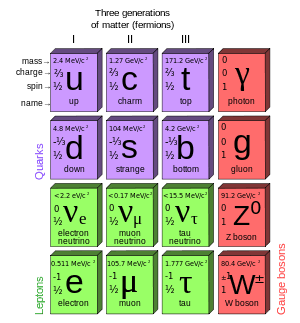
\includegraphics[width=6.0cm]{Fundamental_Particles}
\centering
\caption{The fundamental particles of the Standard Model\cite{Patrignani:2016xqp}.}
\label{fig:fundpart}
\end{figure}
\par
The Standard Model is the unification of the three symmetry groups, SU(3) x SU(2) x U(1), representing the strong, weak, and electromagnetic forces respectively\cite{Langacker:2009my}.  In terms of scientific accomplishments, the Standard Model is one of the most tested theories of nature with an agreement between the theory and observed results up to ten digits\cite{Aoyama:2014sxa}.  Even though the Standard Model gives us a deep understanding of many natural phenomena and has a wide range of uses; from understanding the evolution of the Big Bang, the bonding of atoms and molecules, and the nature of light, to cancer treatments and nuclear security, it is fundamentally an incomplete theory of nature.  The fact that Gravity has yet to be unified into a quantum theory tells us that the Standard Model is incomplete.  High energy experiments give us some of the most extreme conditions possible to test the Standard Model and to look for phenomena outside of the theory.  Are there new symmetries and laws that manifest at high energies? Can we create dark matter or dark energy in a laboratory?  Are quarks and leptons fundamental or finite in size?  Do the four fundamental forces emerge from some yet unknown unified force?  And why is antimatter absent in the Universe?  All of these open questions are of great interest and currently form large areas of active research.  

\par
The theory of strong interactions, Quantum Chromodynamics(QCD), is described by the SU(3) group and is analogous to Quantum Electrodynamics (QED) with gluons being the force mediator instead of photons and quarks carrying mass.  Quarks and gluons are colloquially known as partons and are particles that interact via the strong force.  At low energies and over large length scales, partons are confined to a color neutral state and these particles must clump together into color neutral hadrons.  As two colored partons begin to separate, at some point it becomes energetically favorable to create a quark--antiquark pair out of the vacuum rather then expanding the distance between neighboring partons.  Due to confinement, quark interactions at high energy collider experiments manifest themselves as a spray of hadrons known as a `jet'.  The other main attribute of QCD is asymptotic freedom, as the interactions between partons become more energetic and the length scale decreases, the strong coupling constant becomes exceedingly small, $ \alpha_{strong} << 1$, and the partons freely interact with one another.  Due to asymptotic freedom nuclear matter undergoes a phase transition called the Quark--Gluon Plasma (QGP) at high energies and densities. 



%The theory of strong interactions, Quantum Chromodynamics(QCD), is described by the SU(3) group and similar in analogy to the electric charge of Quantum Electrodynamics carries color charge, red green, blue.

%Nuclear collisions, were the strong coupling constant becomes vanishingly small, allows for 
%\par 
%The Large Hadron Collider(LHC) is the largest and most powerful particle collider ever built.  In 2012 it gained world wide attention for the discovery of the Higgs Boson made by the Compact Muon Solenoid(CMS) and A Toroidal LHC ApparatuS(ATLAS) experiments.  By colliding lead atoms with one another the LHC is able to achieve the temperatures and energy densities necessary to create the QGP.  However, at the LHC the QGP only has a mean lifetime of $ ~ 10^{-23}$  seconds and thus measuring the properties of this phase of matter is difficult and must be infered by the final state particles that reach the detectors. Jets are an attractive tool for measuring the properties of the QGP because they created during the earliest stages of a heavy ion collision


\par
This thesis will present an overview of Quantum Chromodynamics in Chapter 2, with an emphasis on jet physics and heavy ion collisions.  Chapter 3 will give a brief overview of the Large Hadron Collider and the ALICE experiment, including the relevant subsystems for this jet analysis.  Chapter 4 will discuss the contribution to the upgrade of the ALICE Time Projection Chamber performed during my Ph.D. studies.  Chapter 5 will discuss the analysis methodology and corrections to the data.  Finally, Chapter 6 will present the final fully corrected results along with comparisons to theoretical calculations and previous measured observations and also act as a final discussion, outlook, and conclusion. 
    %Fucking left quote symbol ` and not '    

\chapter{Quantum Chromodynamics} \label{ch:qcd}
In 1968 deep inelastic scatterings performed at the Stanford Linear Accelerator Center showed that the proton had internal structure\cite{Riordan1287} called partons at the time.  Within a decade of this discovery the partons were broken into two categories: the mass carrying fermions were known as the quarks and the gauge boson force carriers were called gluons.  The interactions of these two types of particles were described by the quantum field theory known as Quantum Chromodynamics (QCD) and by the SU(3) symmetry group.  SU(3) guarantees that color charge is conserved and this results in quarks grouping together into `colorless' hadrons.

\section{The QCD Lagrangian}
QCD is the strongest of the known fundamental forces.  It is a gauge field theory described by the Lagrangian density

\begin{equation}
{\cal L}=-\frac{1}{4}F^{\alpha}_{\mu\nu}F^{\mu\nu}_{\alpha}
- \alpha_{s} (\bar{q}_{j}\gamma_{\mu}T_{\alpha}q_{j})G_{\alpha}^{\mu}
+ \bar{q}_{j}(i\gamma^{\mu} \partial_{\mu} - m)q_{j}
\label{eq:lagrangian}
\end{equation}

\noindent
where $q$ and $\bar{q}$ represent the color/anti-color fields summed over color $j$, $\alpha_{s}$ is the strong coupling strength,$\gamma^{\mu}$ is the Dirac gamma matrix, $G_{\alpha}^{\mu}$ is the gauge field for color \textit{$\alpha$}, $G_{\alpha}^{\mu}$ is similar in analogy to the \textbf{W} matrix from the electroweak theory.  $F^{\alpha}_{\mu\nu}$ is the field strength tensor and it describes the gluon interactions. The first term of the Lagrangian is the gluon contribution and carries no mass variable.  The second term describes how quarks and gluons interact with each other. The final term describes quark interactions and the coupling between them and will be explored further in this thesis.

At short distances, less than 0.2 \textit{fm}, the strong coupling constant becomes exceedingly small and the second term of the Lagrangian displays an important property known as asymptotic freedom\cite{Wilczek:2005az}.  Numerically the strong coupling constant is given as,

\begin{equation}
\alpha_{s} = \frac{1}{\beta_{0} \; \ln(Q^{2}/\Lambda^{2} )}
\label{eq:alpha_s}
\end{equation}

\noindent
where $\alpha_{s}$ is the strong coupling constant, $Q^{2}$ is the momentum transfer between two interacting partons, $\Lambda^{2}$ is a cutoff below which QCD phenomena are strongly suppressed, and $\beta_{0}$ is a scale factor.  Figure \ref{fig:as} shows the value of $\alpha_{s}$ as a function of the momentum transfer measured from various particle experiments and clearly shows the decreasing strength at high energies.

\begin{figure}[h]
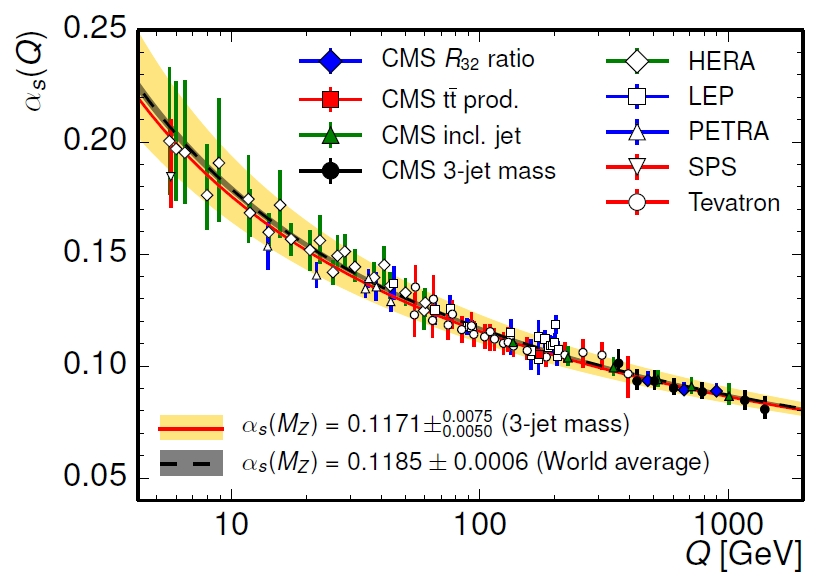
\includegraphics[width=12.0cm]{alphas_s}
\centering
\caption{Strong coupling constant ($\alpha_{s}$) as a function of the momentum transfer (Q)\cite{CMS:2014mna}.}
\label{fig:as}
\end{figure}

\section{Jets}

Hard probes (large $Q^{2}$ interactions), are produced in the earliest stages of a high energy collision when the largest momentum transfer processes occur.  The interaction and scattering of partons is a 2 $\rightarrow$ 2 process, meaning that two partons will interact and the outgoing partons also come in pairs.  As two highly energetic partons propagate away from one another they will instigate a shower of daughter partons via gluon radiation and the generation of low-mass $q \bar{q}$\, pairs.  These daughter partons will go on to form collomated sprays of hadrons known as a `jet'.  If the jet was created in a high energy experiment, the final state hadrons will be recorded as tracks in a tracking detector or energy deposits in a calorimeter.  This process is shown in Figure \ref{fig:MakeAJet}.



\begin{figure}[h]
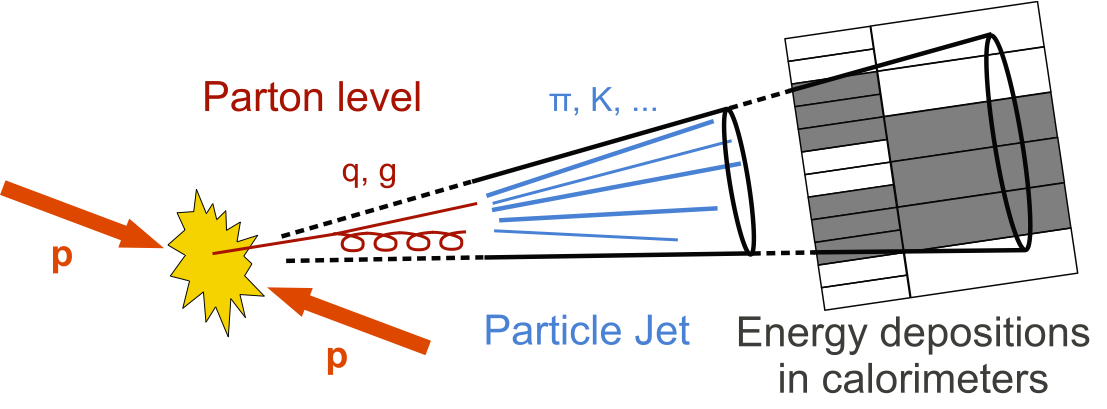
\includegraphics[width=12.0cm]{jetsatcmsand}
\centering
\caption{Diagram showing a jet created by two partons undergoing a hard scattering, forming into hadrons, and detected in a calorimeter\cite{JetPic}.}
\label{fig:MakeAJet}
\end{figure}

The physicist James Daniel Bjorken postulated that a correlation could be surmised by summing over the final state transverse momentum of the hadrons that form a jet to the parton that initiated the hard scattering\cite{PhysRev.179.1547}\cite{Bjorken:1973kd}.  This has led to jets becoming the work-horse for both experimentalists and theorists over the past 30 years in probing QCD phenomena.  This thesis makes use of jets as an important probe of QCD and the following sections are devoted to developing a background for both the theoretical and experimental treatment of jet physics.  The following sections of this chapter will be devoted to the background of jet production.

\subsubsection{Jet Production and The Factorization Theorem}\label{sec:fac}

Due to confinement bare quarks are unobserved, therefore experimentalists must probe QCD interactions by detecting the color neutral final state hadrons measured in collider experiments.  The factorization theorem allows for the final state jet cross section to be broken into a number of steps that can either be calculated pertubatively using pQCD or modeled phenomenologically.  Using the factorization theorem the jet cross section in a pp collision is:


\begin{equation}
d\sigma^{pp \rightarrow jet} \sim f_{a/A}(x_{1},Q^{2}) \otimes  f_{b/B}(x_{2},Q^{2}) \otimes d\sigma_{ab \rightarrow c + X} (x_{1},x_{2}) \otimes D_{c \rightarrow h/jet}(z,Q^{2})
\label{eq:xsection}
\end{equation}

\noindent
Breaking Equation \ref{eq:xsection} down we have:

\begin{itemize}
\item  $ f_{a/A}(x_{1},Q^{2})$ and $ f_{b/B}(x_{2},Q^{2})$ are the parton distribution functions (PDF) that describe the probability of finding parton, \textit{a} or \textit{b}, within nuclei, \textit{A} and \textit{B}, with a given momentum fraction, $x = p_{parton} / p_{hadron} $ as a function of $Q^{2}$.
\item  $d\sigma_{ab \rightarrow c + X} (x_{1},x_{2})$ is the pQCD parton-parton cross section due to the hard scattering of the two partons, \textit{a} and \textit{b}, to an intermediate parton (\textit{c}).
\item   $ D_{c \rightarrow h/jet}(z,Q^{2})$ is the fragmentation function (FF) that describes the probability that an outgoing parton, \textit{c}, fragments and hardonizes into a final state hadron, \textit{h}, within a jet with momentum fraction, $z \equiv p_{hadron} / p_{parton}$.
\end{itemize}

\afterpage{%
\begin{figure}[h]
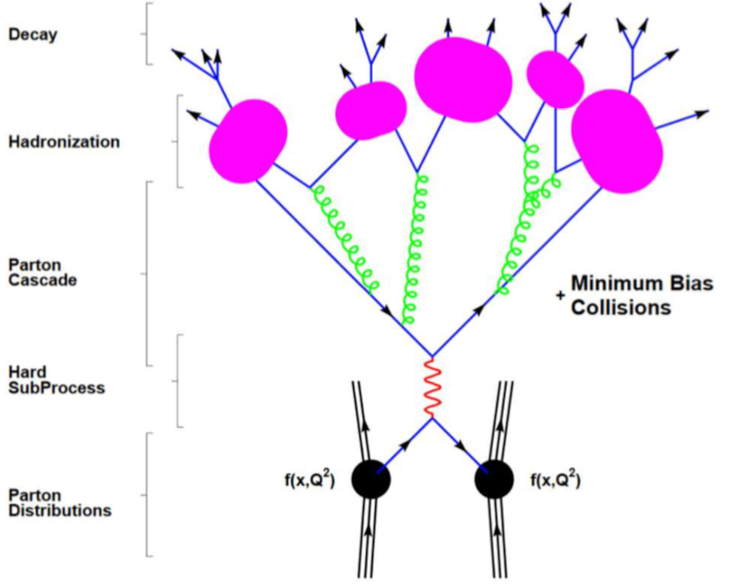
\includegraphics[width=\linewidth]{ppcollison}
\centering
\caption{Schematic of a proton-proton collision.  Starting from the bottom, two partons confined within the colliding protons have a hard interaction.  The outgoing partons will induce partonic showers by radiating quarks and gluons.  The partonic showers will eventually form into final state hadrons, due to confinement, which are measured in high energy experiments\cite{Dobbs:2001ck}.}
\label{fig:FactorizationCartoon}
\end{figure}
\clearpage
}

\noindent
Figure \ref{fig:FactorizationCartoon} shows a cartoon of a pp collision broken into the relevant steps in accordance with the factorization theorem.  The best place to test QCD phenomena using hard probes, i.e. jets, is at high energy hadron colliders, such as those found at CERN\footnote{Discussed in detail in Chapter 3}, Fermilab, and BNL. The time scale that a hard probe is created in a high energy collision is on the order of $\tau \approx 1/p_{T} \approx$ \, 0.1 fm/\textit{c} at $p_{T} = 1 \,$ GeV, which corresponds to some of the earliest stages of the nuclear collision.  The factorization theorem is an incredible tool for understanding high energy interactions and the following sections will discuss the important concepts enveloped in it.

\subsubsection{Parton Distribution Functions}
The PDF occurs twice in Equation \ref{eq:xsection} due to the two partons that will undergo the hard scattering being confined in two different protons.  PDFs convey the structure of a nucleon in terms of the number of flavored quarks or gluons ($u(x)$, $d(x)$, $s(x)$, $\overline{u}(x)$, $\overline{d}(x)$, $\overline{s}(x)$, $g(x)$) and must obey certain constraints and summation rules.  In the case of a proton, with electric charge (\textit{e} = +1),

\begin{equation}
+1 = \frac{2}{3} \int_{0}^{1} [u(x) - \overline{u}(x)] dx - \frac{1}{3} \int^{1}_{0} [d(x) - \overline{d}(x)] dx
\label{eq:PDFcharge}
\end{equation}

\noindent
and isospin (\textit{I} = 1/2),

\begin{equation}
\frac{1}{2} = \frac{1}{2} \int_{0}^{1} [u(x) - \overline{u}(x)] dx - \frac{1}{2} \int^{1}_{0} [d(x) - \overline{d}(x)] dx
\label{eq:PDFIso}
\end{equation}

\noindent
have a solution,
\begin{equation}
 \int_{0}^{1} [u(x) - \overline{u}(x)] = 2
\label{eq:PDFSouU}
\end{equation}

\begin{equation}
\int^{1}_{0} [d(x) - \overline{d}(x)] dx = 1
\label{eq:PDFSouD}
\end{equation}

\noindent
This corresponds to the classical partonic view that protons contain two up quarks and a down quark similarly, and similarly the neutron, with charge \textit{e} = 0 and isospin I = -1/2, is composed of two down quarks and an up quark.  Naively, we could assume that the three quarks composing a proton would each carry a momentum fraction of approximately 1/3 the total momentum of a proton.  However, high energy deep inelastic scattering experiments conducted at the Stanford Linear Collider in the 1960's\cite{Panofsky:871460} measured the momentum carried by the three quarks as only accounting for about 1/2 the total proton momentum.  This led to a more complex and dynamic model of the proton structure with the other half of the proton momentum being carried by neutral partons, which would eventually become known as gluons.

\begin{figure}[h]
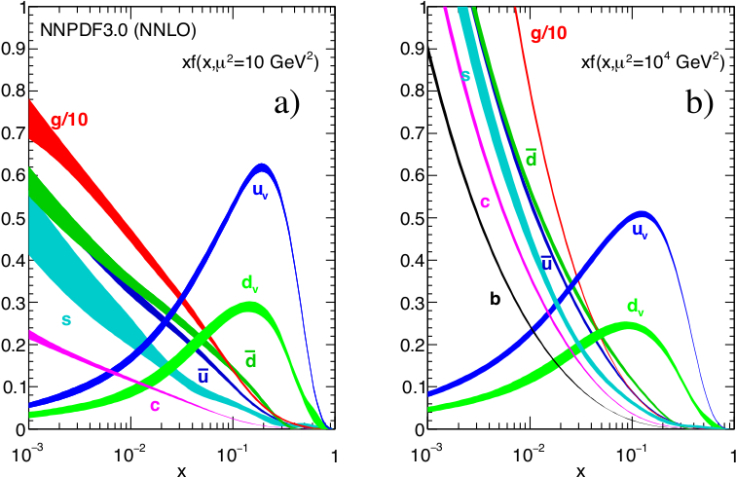
\includegraphics[width=12.0cm]{aOzz6}
\centering
\caption{Proton PDF at $Q^{2}$ = 10 GeV (left) and  $Q^{2}$ = 10 TeV (right) from the NNPDF Collaboration\cite{Feltesse:2010}.}
\label{fig:PDFNNPDF}
\end{figure}

Determining the structure of the partons making up a nucleon is a major endeavor by both theorists and experimentalists.  Two of the most popular PDFs available to physicists are the CTEQ\cite{Kovarik:2013sya} (Coordinated Theoretical-Experimental Project on QCD) and the NNPDF\cite{Ball:1966481} (Neural Network Parton Distribtuion Function) sets.  Figure \ref{fig:PDFNNPDF} shows the proton PDF as a function of the momentum fraction for two energy ranges.  At high values of \textit{x}, the two up quarks account for about 2/3 of the momentum fraction while the down quark accounts for about 1/3 of the total momentum.  These quarks are collectively called the valence quarks.  At high energies (low values of \textit{x}) we see that the proton has non negligible contributions from gluons, anti-quarks, strange, and even charm quarks.  These are collectively known as the sea partons.  Today, the modern picture of a proton's structure is mostly composed of gluons and sea quarks at low values of \textit{x} and this domination only increases as a function of $Q^{2}$\cite{Fritzsch:1992mu}.

\subsubsection{Parton-Parton Cross-Section}
The quark-pquark, quark-gluon, and gluon-gluon cross section can be calculated using perturbation theory.  To the zeroth order in $\alpha_{s}$ this cross-section would be a simple quark-antiquark annihilation and would be calculable using Feynman diagrams as seen in Figure \ref{fig:qqbar}\cite{Collins:1989gx}.  Higher ordered contributions, such as the creation of virtual gluons, require the hard cross-section to be expanded as a series in terms of $\alpha_{s}$.  Calculations of the hard cross-section that incorporate these higher order terms are known as \textit{next-to-leading order} (NLO) with N denoting the number of terms after the leading order that have been included in the cross-section calculation.  Various calculations of the hard cross-section of different QCD processes have been performed over the years typically using either power series or logarithmic expansions of $\alpha_{s}$\cite{Brambilla:2006wp} and corrections for LO, NLO, and even NNLO constitutes a very active field in high energy physics.  Perturbative techniques of the hard cross-section have been extremely successfully in describing jet features in hadronic collisions\cite{Fritzsch:1992mu}.

\begin{figure}[h]
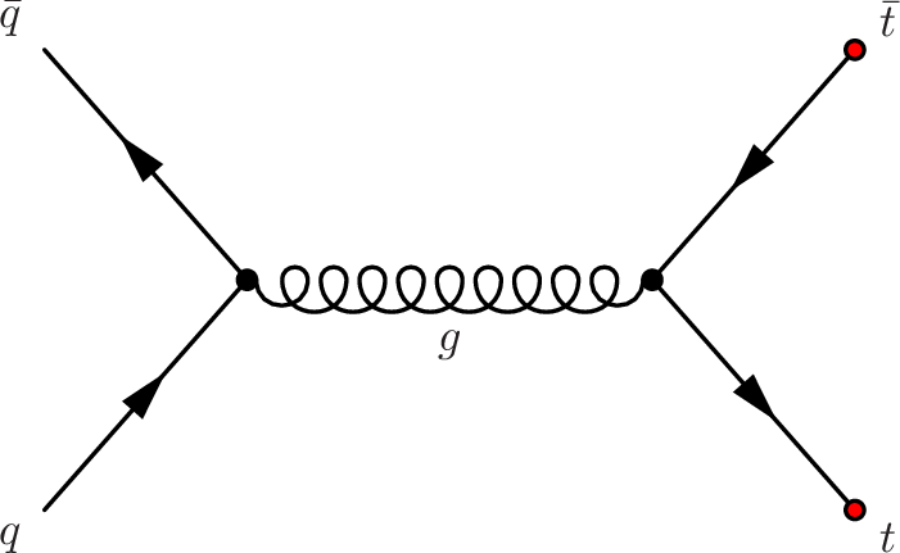
\includegraphics[width=6.0cm]{Ttbar_production_via_qqbar_annihilation}
\centering
\caption{Lowest order quark-antiquark annihilation to top-antitop pair\cite{Erdmann:2001ne}.}
\label{fig:qqbar}
\end{figure}

\subsubsection{Hadronization}

Hadronization, the process by which the colored pQCD partons form into colorless non-pQCD hadrons, represents a significant barrier in progressing jet physics.  This is due to the fact that hadronization encompasses several smaller processes, which in themselves are hard to characterize. Thus, like PDFs, an accurate description of hadronization requires a phenomenological approach by which experimental results help complement theoretical calculations.  Jet production via hadronization\cite{Webber:1994zd} follows two distinct stages.  First, the partons that underwent a hard scattering start to emit radiation via gluon bremsstrahlung up until time, $t < Q^{2}$.  This is known as the parton cascade.  The parton cascade is the precursor to a jet as most of the radiation generated will travel in the same direction as the initial hard scattered parton.  However, this immediately poses an issue in jet physics as radiation generated at a wide angle away from the momentum axis of the initial hard scattered parton will not be associated with the jet.

\begin{figure}[h]
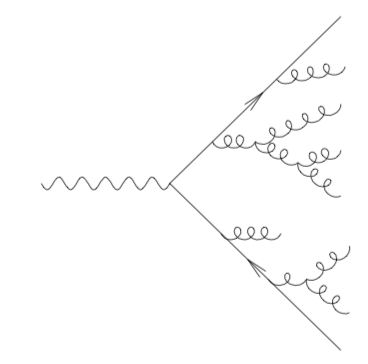
\includegraphics[width=8.0cm]{partoncascade}
\centering
\caption{Parton cascade in a hadronic collision\cite{Webber:1994zd}.}
\label{fig:pcascade}
\end{figure}

\noindent
After the cascade has ended, the partons form into color neutral hadrons.  There are two main phenomenological models used to describe the hadron forming process, the Lund String Model and the Cluster Hadronization Model.  

The QCD potential is

\begin{equation}
V(r) = - \frac{\alpha_{s}}{r} + \sigma \, r
\label{eq:QCDPotential}
\end{equation}

\noindent
where the first term of Equation \ref{eq:QCDPotential} is similar to the Coulomb potential with a 1/r dependence and is the dominate term at short distance.  The second term has a string-like potential with $\sigma$ referring to a string-like tension.  The Lund String Model uses this potential, ignores gluon radiation, and has fragmentation occur via breaking the string tension with the production of $q\overline{q}$ sea quarks.  The created sea quarks will carry some momentum fraction, z, of the initial parton until z falls below some cutoff.  Figure \ref{fig:qqbarstring} shows two quarks undergoing a string breaking, each of the quarks initiating the string breaking will combine with a sea quark in an iterative manner to form hadrons.  


\begin{figure}[h]
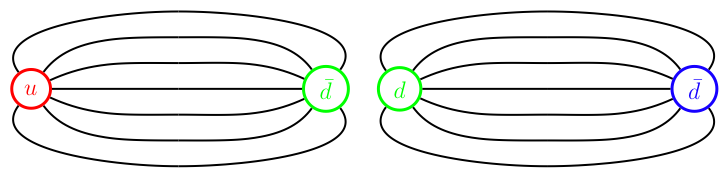
\includegraphics[width=15.0cm]{qqbarproductionvaccum}
\centering
\caption{$u \overline{d}$ generating a $d \overline{d}$ pair via string breaking which will form color neutral hadrons, black lines show the string like equipotentials.\cite{Andersson:2002ap}.}
\label{fig:qqbarstring}
\end{figure}

The Cluster Hadronization Model has gluons splitting after the parton cascade phase into $q\overline{q}$ pairs.  These pairs will form color-singlet clusters with other neighboring quarks in phase-space.  These color-singlets will typically be a few GeV/\textit{$c^{2}$} in mass and are treated as excited meson resonances.  These psuedo-resonances will decay via their normal branching ratios into the stable hadrons\cite{Webber:1983if}.

\subsubsection{Fragmentation}

Similar to the way a PDF quantitatively describes the structure of a nucleon, the fragmentaion function (FF) quantitatively describes the hadronization process.  The FF is also similar to the PDF in that it is also a probability distribution, thus it follows the probabilistic rule that

\begin{equation}
\sum \int_{0}^{1} z D_{c \rightarrow \, h/jet} (z,Q^{2})dz = 1
\label{eq:FFRule}
\end{equation}

\noindent
where the sum is carried over the particles constituting the jet, $c \rightarrow h/jet$ states that the function in question is only concerned with a parton, c, fragmenting into a final state particle, h, that is part of a jet.  The fractional momentum of the hadrons created from the fragmenting parton, $z \equiv p_{hadron} / p_{parton}$, is an exponentially decreasing distribution between 0 and 1 which shows how fragmented hadrons carry the partial energy from the initial parton scattering.  Parton-Hadron Duality\cite{Jenkovszky:2012dc} states that the leading hadron should correlate with the kinematic properties associated with the hard scattered quark that initiated the jet.  Thus we can measure the fragmentation function as $z = p_{hadron} / p_{jet}$.  The formulation of the FF as the fractional energy carried by the hadrons in a jet was a breakthrough in pQCD techniques and is analogous to the way an electron passing through an absorber creates photon showers. These photons continue generating conversion electrons until the total energy has been dissipated into the material.

\begin{figure}[h]
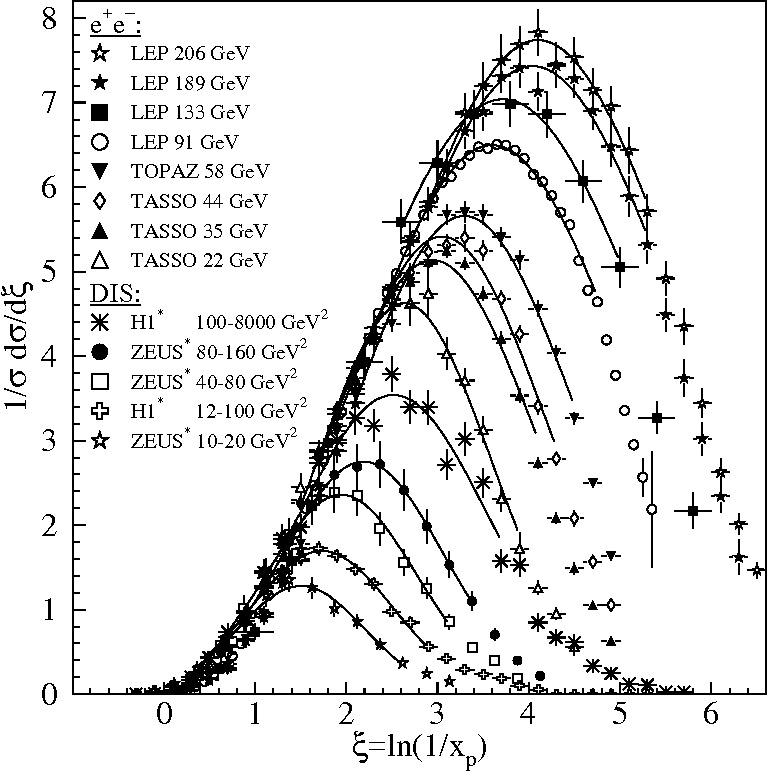
\includegraphics[width=8.0cm]{FFfunctions}
\centering
\caption{Fragmentaion functions from $e^{+}e^{-}$and DIS experiments with fits\cite{rak_tannenbaum_2013} as a function of the total cross-section, $\sigma$.}
\label{fig:FFfunc}
\end{figure}


Figure \ref{fig:FFfunc} is the FF in terms of the Gaussian equation, with $\sigma$ refering to the total cross-section, $z \, dN/dz = - dN /d \xi $, and $\xi = -ln  \,1/z_{p}$. The Gaussian peaks in Figure \ref{fig:FFfunc} along with the suppression of the FF at low z values due to gluon coherence were predicted by pQCD. 

\section{Jet Finding Algorithms}

A jet arises from the fragmentation of a hard parton to final state hadrons.  However, grouping the hadrons together into a jet is ambiguous.  Jet finding algorithms are used because they standardized the definition between theorists and experimentalists and give results comparable to each other. Early on in jet physics, both theorists and experimentalists used a wide variety of jet finders and definitions which made comparisons between experiments or to theoretical calculations nearly impossible\cite{Atkin:2015msa}.  For example, a radiated gluon that splits into a quark anti-quark pair may become one or two jets depending on the angular separation and the algorithm used.  Early jet finders tended to be sensitive to soft particles or could give widely varying yields to the number of jets in an event.  In 1990, the Snowmass Accord\cite{Huth:217490} reached a standardized definition of a jet between experimentalists and theorists.  The agreement maintained that any algorithm that clusters particles into a jet must be both infrared and collinear safe (IRC).  

\begin{figure}[h]
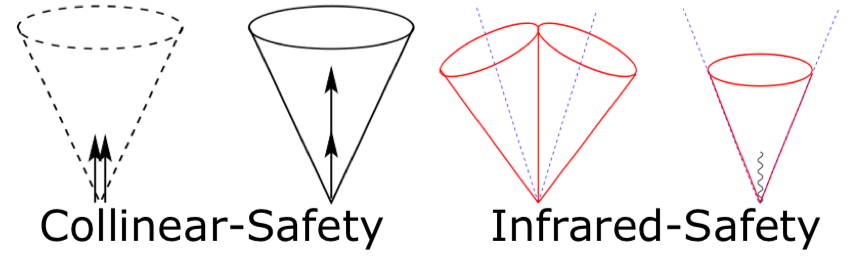
\includegraphics[width=15.0cm]{IRCsafe}
\centering
\caption{Cartoon showing collinear and infrared safe jet candidates\cite{Blazey:2000qt}.}
\label{fig:IRCsafe}
\end{figure}

A hard, high momentum transfer, scattered parton will undergo collinear splittings, emissons of gluons, as part of the fragmentation process.  This is a difficult process to model theoretically so jet finding algorithms maintain collinear safety.
Collinear safety ensures jets remained unchanged due to any gluon emissions.  Infrared safety in turn requires that the emission of soft radiation should not affect jet.  This makes jets returned by the algorithm  a signature of a hard process.  Both of these processes are shown in Figure \ref{fig:IRCsafe}. After the adoption of these standards from the Snowmass Accord, old algorithms that violated these rules were patched and new jet finders were developed to comply with IRC safety.  The most prevalent jet finding algorithms today fall into two categories: cone algorithms and sequential recombination/clustering algorithms.

\subsubsection{Cone Algorithms}

Cone algorithms made up the bulk of early jet finders.  The only IRC safe cone algorithm still in use today is the seedless infra-red safe cone algorithm (SIScone).  SIScone defines a cone of radius R around the highest momentum particle in the coordinates of $(\eta,\phi)$\footnote{It is possible to use a Cartesian coordinate system in particle colliders, with the z-component referring to points along the beam axis while the xy-plane is perpendicular to the beam axis.  However, this system is not invariant under a Lorentz boost.  Therefore it is more useful to use the cylindrical-like coordinates of psuedorapidity ($\eta$) and the azimuth angle ($\phi$). Psuedorapidity may be thought of as the polar angle in a cylindrical coordinate system with $\eta = 0$ when the polar angle is perpendicular to the beam axis and $\eta = \infty$ along the beam axis.  $\phi$ is the azimuth angle that rotates around the beam axis.  Both, $\eta$ and $\phi$ are invariant for Lorentz boosts along the beamline and allow for easy comparisons between the center-of-mass frame and the laboratory frame of a high energy collision.}.  This is the proto-jet.  SIScone then proceeds through an iterative process of finding all the particles within the jet radius such that $R \leq \sqrt{\phi^{2} + \eta^{2}}$ and calculates a new jet center based on these particles' momenta and a new weighted jet axis$(\eta,\phi)$.  If the new center matches the proto-jet center, the proto-jet is tagged as a stable jet.  All the particles in that jet are removed and SIScone moves onto the next highest $p_{T}$ particle.  Cone algorithms tend to be unpopular due to being computationally expensive, difficult to implement theoretically, and can give results not calculable in perturbation theory.

\subsubsection{Sequential/Recombination Algorithms}

The other class of jet finders are the sequential/recombination algorithms, which are favored by experimentalists and theorists, and are IRC safe.  There are three sequential/recombination algorithms: $k_{T}$, Anti-$k_{T}$, and the Cambridge/Aachen jet finders, with $k_{T}$ referring to the component of a jet constituent's momentum perpendicular to the jet axis.  All of the algorithms use a similar method.  First they find the distance between every pair of particles, $d_{i,j}$,  such that



\begin{equation}
d_{i,j} = min[p^{a}_{T,i},p^{a}_{T,j}] \, \frac{\Delta^{2}_{ij}}{R^{2}}
\label{eq:JetAlgo}
\end{equation}

\noindent
where $p^{a}_{T,i}$ is the transverse momentum of particle \textit{i}, \textit{a} is free parameter that is set based on which algorithm is used, $\Delta^{2}_{ij} = (\eta_{i} - \eta_{j})^{2} + (\phi_{i} + \phi_{j})^{2}$ is the distance between the particles, and R is the radius of the jet.  A second distance is defined in the sequential/recombination algorithm scheme,

\begin{equation}
d_{i,B} = p^{a}_{T,i}
\label{eq:MinJet}
\end{equation}

\noindent
which is only a function of the particles transverse momentum.  Sequential/Recombination algorithms find the set of all particles, ${d_{i,j},d_{i,B}}$, such that if $d_{i,B}$ is the minimum for particle \textit{i} it is tagged as a jet and removed from the list.  If $d_{i,j}$ are a minimum for particles \textit{i} and \textit{j} these two particles are merged together into a new particle (\textit{ij}) and a new minimum is found between (\textit{ij}) and a new particle \textit{k} until all the particles are either merged into jets or the minimization function is no longer satisfied.

\subsubsection{$k_{T}$ Algorithm}
The $k_{T}$ algorithm sets the value \textit{a} to 2, this results in a minimization function,

\begin{equation}
d_{i,j} = min[p^{2}_{T,i},p^{2}_{T,j}] \, \frac{\Delta^{2}_{ij}}{R^{2}}
\label{eq:kt}
\end{equation}

\noindent
which clusters low momentum particles first, making this algorithm susceptible to the underlying event, UE, or pile-up, PU.  Thus the $k_{T}$ algorithm is good at estimating any background present in a high energy collision. 

\subsubsection{Anti-$k_{T}$ Algorithm}
The Anti-$k_{T}$ algorithm sets the value \textit{a} to -2, resulting in a minimization function,

\begin{equation}
d_{i,j} = min \Bigg [\frac{1}{p^{2}_{T,i}}, \frac{1}{p^{2}_{T,j}} \Bigg ] \, \frac{\Delta^{2}_{ij}}{R^{2}}.
\label{eq:Akt}
\end{equation}

The minimization function begins with high-$p_{T}$ particles, thus the area and axis of a jet is only slightly perturbed by soft particles.  This makes the Anti-$k_{T}$ algorithm robust in jet finding with events having pile-up.  The Anti-$k_{T}$ algorithm is the default jet finding algorithm used at the Large Hadron Collider and is the one used in this thesis.

\subsubsection{Cambridge/Aachen Algorithm}

The Cambridge/Aachen algorithm sets \textit{a} to 0 and this results in a minimization function of,

\begin{equation}
d_{i,j} = \frac{\Delta^{2}_{ij}}{R^{2}}
\label{eq:CBalg}
\end{equation}

\noindent
which makes it independent of particle momentum and sensitive to PU and the UE.  Due to the fact that the Cambridge/Aachen algorithm is only dependent on the particle coordinate it is most useful in studying jet structure.

Figure \ref{fig:AllJetFinder} shows the jets found in a single event using all four jet finding algorithms.  It should be noted that the Cambridge/Aachen and $k_{T}$ algorithms have highly irregular and large shapes, making them both susceptible to the presence of a UE, while SIScone finds an additional jet due to splitting.  The Anti-$k_{T}$ algorithm finds circular jets which demonstrates its' robustness to hard radiation.  

\afterpage{%
\begin{figure}[h]
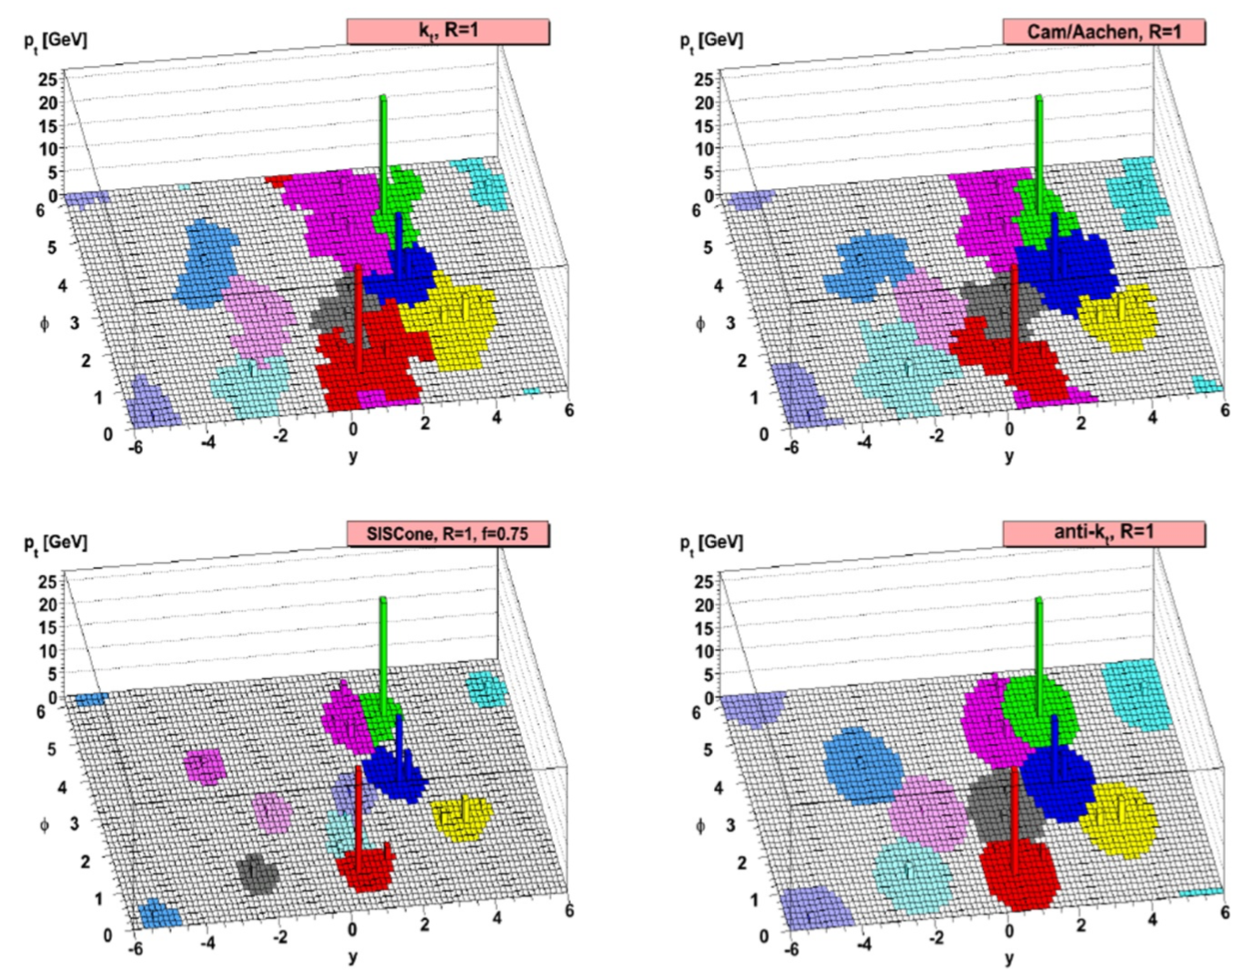
\includegraphics[width=\linewidth]{FastJet}
\centering
\caption{Lego plot of all four jet finders used on a single event with R = 1 jet radius\cite{Atkin:2015msa}.}
\label{fig:AllJetFinder}
\end{figure}
\clearpage
}

Once a stable jet is found, a recombination scheme is deployed in order to garner the jet kinematics.  By adding the 4-vector, $\boldsymbol{p}^{\mu} = (\boldsymbol{E},\boldsymbol{p}_{x},\boldsymbol{p}_{y},\boldsymbol{p}_{Z})$, for all of the associated particles composing a jet, we may obtain the jet momentum, energy, coordinates, etc.  In a particle collider with the tracks from a tracking detector measuring particle momentum and the towers of a calorimeter measuring particle energy we obtain the following relationships



\begin{equation}
p_{T}^{jet} = \sum_{particles} p_{T} = \sum_{tracks} p_{T}
\label{eq:JePt}
\end{equation}

\begin{equation}
E^{jet} = \sum_{particles} E = \sum_{towers} E
\label{eq:JetE}
\end{equation}

\begin{equation}
\eta^{jet} = \frac{1}{2} \, \ln \Bigg (  \frac{|\boldsymbol{p}^{jet}| + p_{L}^{jet}}{|\boldsymbol{p}^{jet}| - p_{L}^{jet}}  \Bigg )
\label{eq:JetEta}
\end{equation}

\begin{equation}
\tan \phi^{jet} = \frac{p_{y}^{jet}}{p_{x}^{jet}}
\label{eq:JetPhi}
\end{equation}
\noindent 
where $p_{L}$ refers to the longitudinal momentum which is the momentum component parallel to the beam axis, $\eta^{jet}$ and $\phi^{jet}$ are the jet coordinates in psuedo-rapidity and the azimuth angle.  This method of adding the 4-vector of the particles composing the jet together in order to gain the jet kinematics is known as the E-scheme\cite{Cacciari:2011ma}.

\subsubsection{FastJet}
FastJet\cite{Cacciari:2011ma} is a \verb|C++| software package that performs jet finding.  Due to the computational efficiency, ease of use, and straight forward implementation, FastJet is the preferred jet finding software package used by theorists and current high energy experiments. It implements the four previously discussed jet finders along with both the E-scheme and a boost invariant $p_{T}$ scheme (BIpt-scheme) for recombination.  The BIpt-scheme obtains the jet momentum and energy in the same manner as the E-scheme but uses a weighted average to find the jet coordinates,

\begin{equation}
\eta^{Jet} = \sum_{particle} \frac{p_{T}^{particle}}{P_{T}^{jet}} \, \eta^{particle}
\label{eq:JetEtaRecom}
\end{equation}
\begin{equation}
\phi^{jet} = \sum_{particle} \frac{p_{T}^{particle}}{P_{T}^{jet}} \, \phi^{particle}
\label{eq:JetPhiRecom}
\end{equation}

\noindent
In addition to basic jet measurements, FastJet contains a number of advance features, which allows it to be used to study jet area, jet substructure, and jet background subtraction\cite{Connors:2017ptx}.

\section{Monte-Carlo Generators}
Monte Carlos allow for the simulation of high energy events on a statistical basis.  Particle level generators use different phenomenological models of the factorization theorem in order to simulate the energy, momentum, particle species, multiplicity, and direction of travel expected in a high energy collision.  In this thesis Monte Carlos are also used to understand and correct for inefficiencies due to the experiment using a GEANT simulation of ALICE, this is discussed in more depth in Chapter 5.  The following sections will go over some of the different Monte Carlos used in this thesis and the physics behind how they simulate high energy collisions.

\subsubsection{PYTHIA}

PYTHIA\cite{Sjostrand:2007gs}, is a Monte Carlo software tool-kit used to model proton-proton collisions.  The package uses pre-defined parton distribution functions as input.  Afterwards it simulates the partonic showers and radiation due to a hard scattering by generating the leading-order, LO, scattering matrix elements.  Hadronization is performed in PYTHIA using the Lund String Model.  The final state hadrons are formed using the branching ratios to decay excited states.

PYTHIA underestimates jet production due to the limitations of using LO calculations.  Therefore, it uses an arbitrary value (K-factor) to make NLO corrections to the LO cross section.  The K-factor is defined as

\begin{equation}
K = \frac{\sigma_{NLO}}{\sigma_{LO}}.
\label{eq:Kfactor}
\end{equation}

NLO corrections to the cross-section will not match experimental results, especially at low energies.  PYTHIA implements additional phenomenological adjustments used to better match data.  PYTHIA encompasses these parameters into sets known as `tunes', with PYTHIA 6.4 Perugia-2010 tune being used for this analysis\cite{Skands:2010ak}.

\subsubsection{PHOJET}
PHOJET is a \verb|FORTRAN 77| Monte Carlo simulator used to model proton-proton collisions. It is an alternative to PYTHIA and is better at modeling soft physics processes present in high energy collisions.   PHOJET implements the Dual Parton model\cite{CAPELLA1994225}\cite{Wong:241251} and multiple parton interactions\cite{Bopp:1998rc} to model soft physics, similar to PYTHIA.  Hard interactions are implemented in PHOJET using LO scattering elements and it uses PYTHIA for the fragmentation and hadronization phase.  Due to its ability to model soft physics, PHOJET is better at comparing to Min Bias\footnote{Events with a low total transverse momentum and high cross section} data and understanding jet results in a low kinematic range.  PHOJET also acts as a benchmark in understanding any bias due to using other Monte Carlo generators, such as PYTHIA.  PHOJET v1.2 is used in this thesis.


\subsubsection{HERWIG}
The HERWIG\cite{Bahr:2008pv} Monte Carlo generator is a \verb|FORTRAN| software package used to generate proton-proton events.  It is similar to PYTHIA in that it calculates the LO hard scattering of partons, however it uses the cluster model of hadronization to produce jets based on gluon splitting.  It is also similar to PHOJET in regards to the evolution of final state jets with soft gluon angular ordering.  By comparing HERWIG, PYTHIA, and PHOJET it is possible to test for sensitivities to jet production in high energy events due to different types of hadronization models and soft radiation.


\section{The Quark-Gluon Plasma}
At the temperatures and pressures typical to the universe today nuclear matter is confined to a colorless hadrons.  However, it was theorized that at extreme temperatures, such as those experienced in the early universe, partons would have undergone a phase transition where they were no longer bound in a color neutral state.  This state of matter would have been analogous to a conventional plasma where the electrons are no longer bound to a nucleus, thus the state was dubbed the Quark-Gluon Plasma (QGP).

The nuclear phase diagram is shown in Figure \ref{fig:QCDphase} as a function of temperature and the net baryon density.  Normal nuclear matter is confined to the bottom left while increasing temperatures and/or densities correspond to the QGP.  Modern particle colliders, such as RHIC and the LHC, are able to obtain the densities and temperatures necessary to create a QGP and are likewise shown in the figure.  The reason for particle colliders being located at low baryon density is due to the fact that at collider energies at mid-rapidity the plasma are dominated by quark-antiquark pairs, so the net baryon density is close to zero.  This dilutes the total baryon density in the initial system and is more akin to what the early Universe was like.  

\begin{figure}[h]
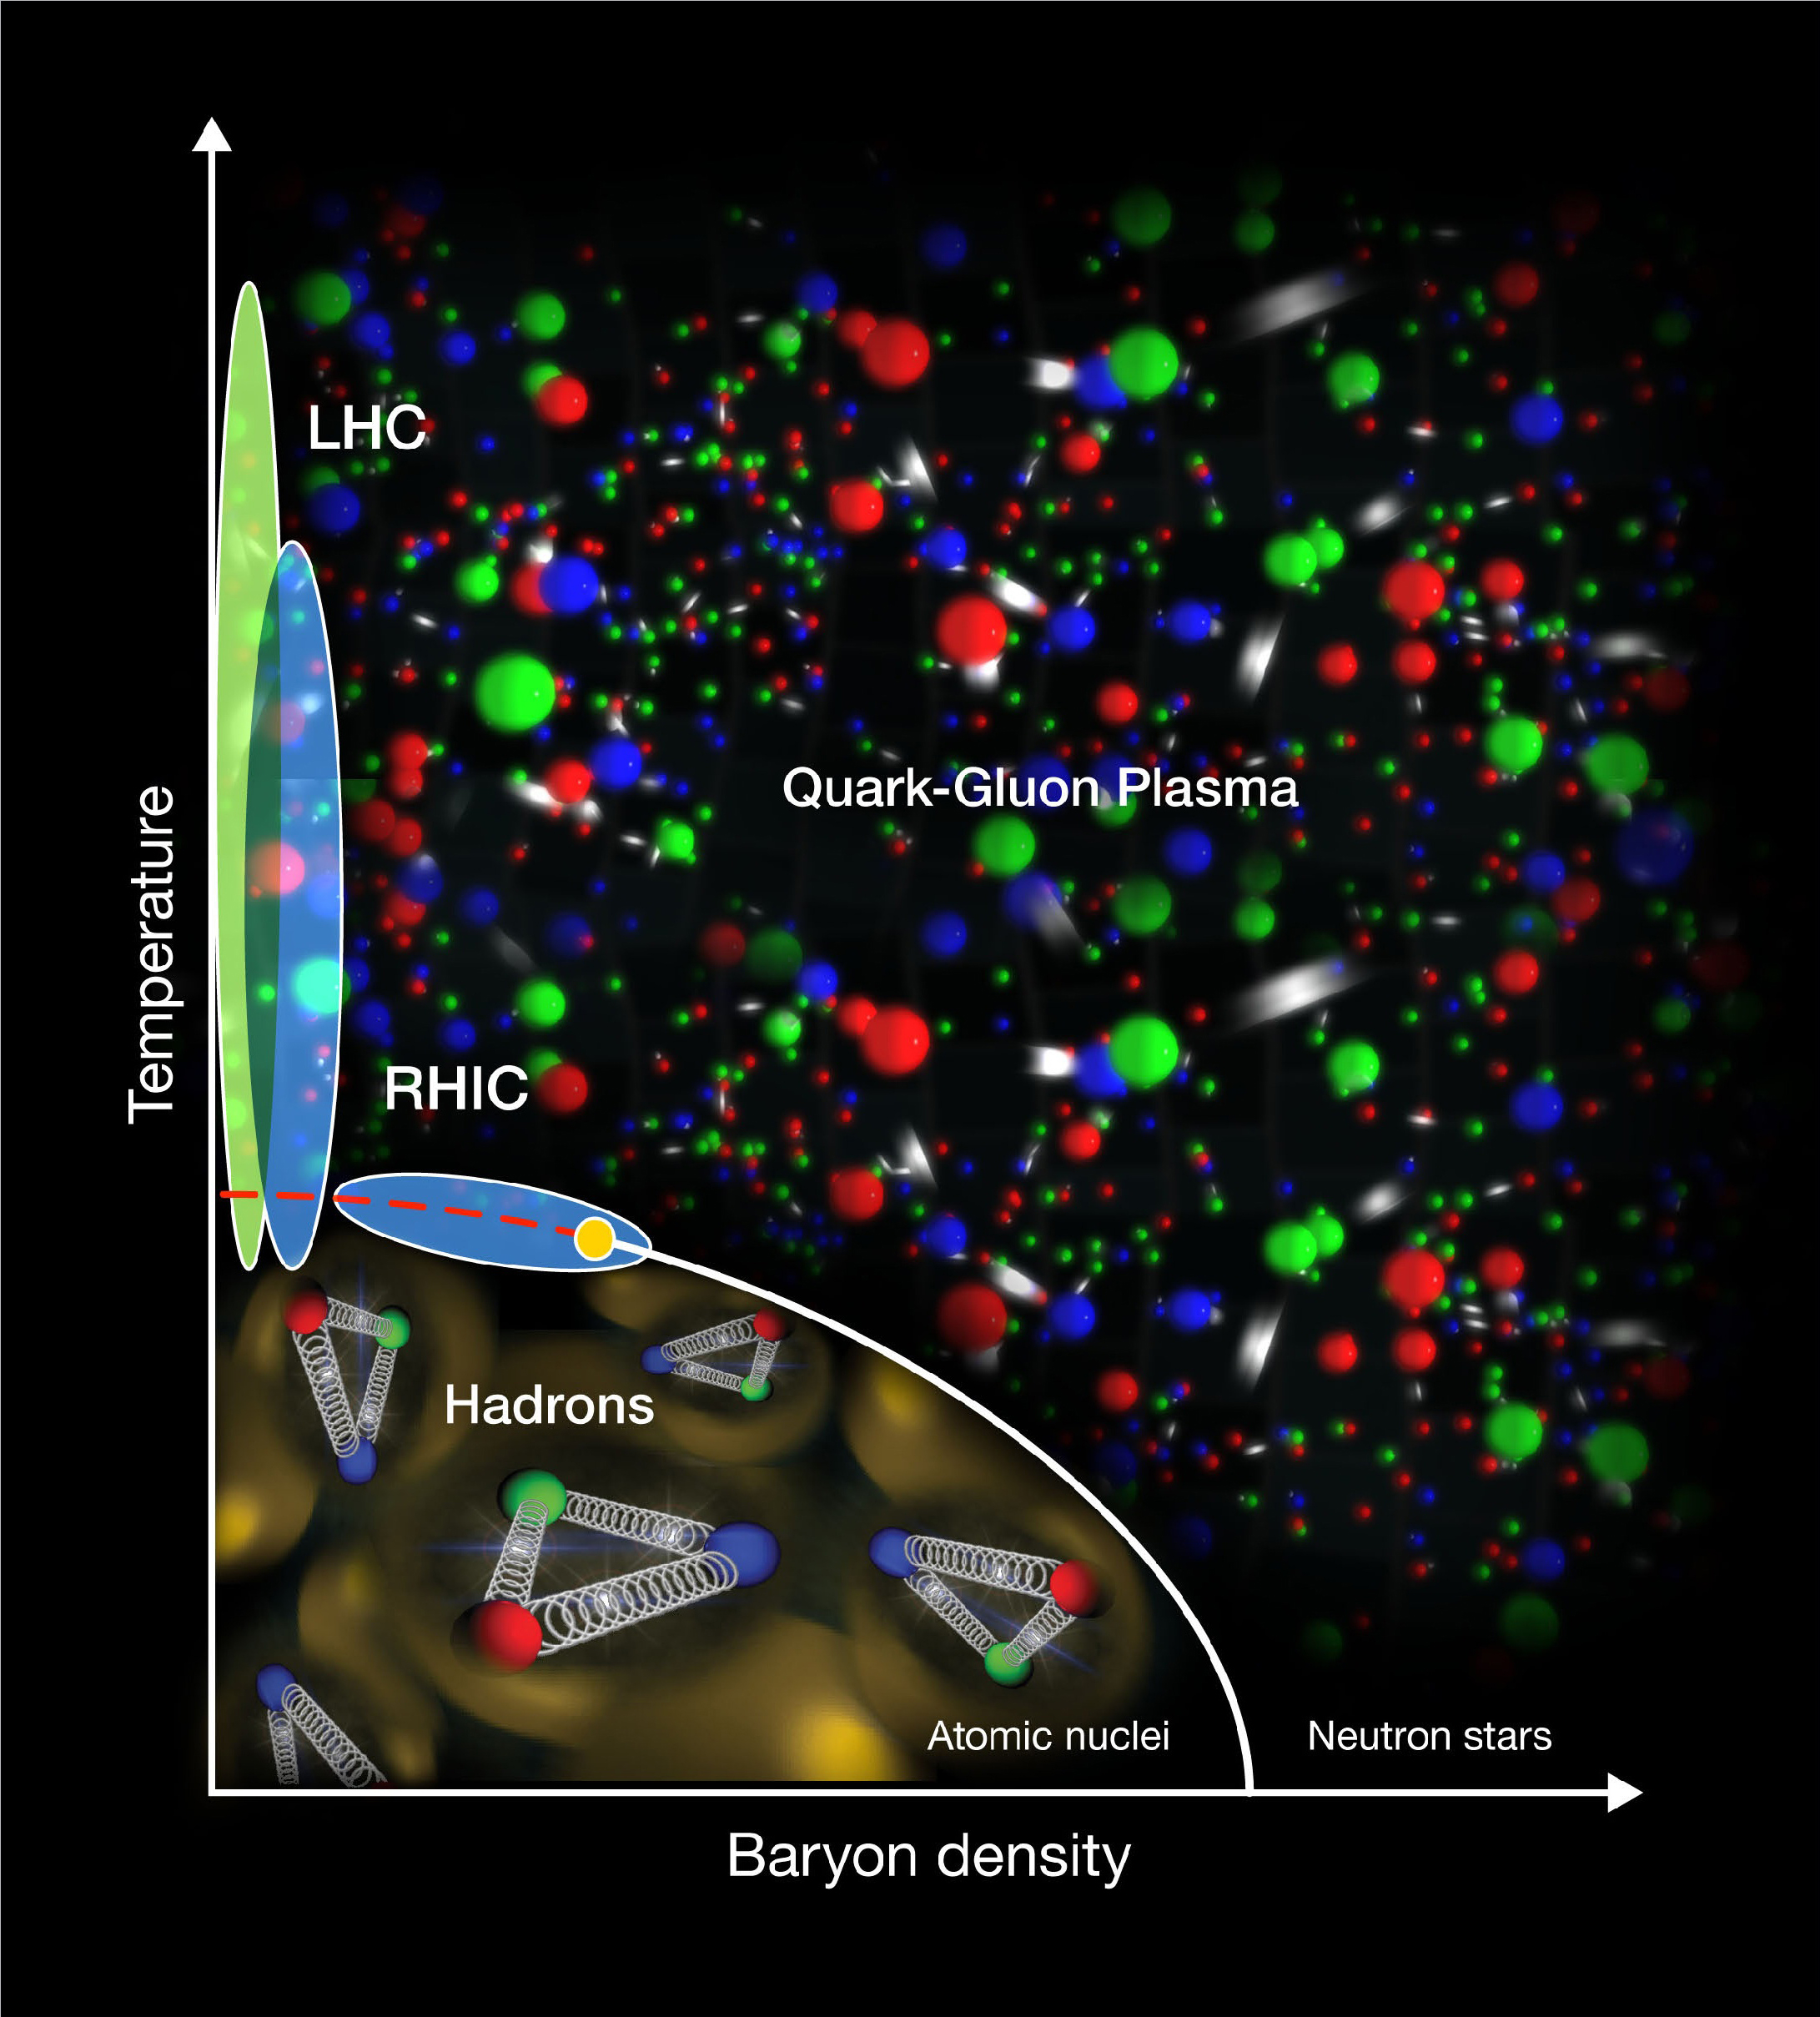
\includegraphics[width=8.0cm]{610_1}
\centering
\caption{The QCD phase diagram\cite{Mohanty:2013yca}.}
\label{fig:QCDphase}
\end{figure}

\subsubsection{Nuclear Collisions}
By colliding heavy nuclei together in high energy colliders it is possible to obtain the energy densities and temperatures associated with the QGP.  The first signatures for the QGP were measured via a J/$\psi$ suppression at the Super Proton Synchrotron, located at CERN in 2000\cite{Csorgo:2000yu}.  In 2005, the four experiments on the RHIC collider: BRAHMS\cite{Arsene:2004fa}, PHENIX\cite{Adcox2005184}, PHOBOS\cite{Back200528}, and STAR\cite{Adams2005102}, co-announced the observation of a new state of matter consistent with the hot and dense QGP.  The results from RHIC indicated that the QGP behaves more like a perfect fluid over a plasma-like state\cite{Jacak310}.

Figure \ref{fig:HeavyIonCollisionvPP} shows the difference between a proton-proton collision and a heavy-ion collision.  The heavy-ion collision mirrors the processes in a proton-proton collision (left) described in depth in Section \ref{sec:fac}.  After the initial hard scattering the phase transition to a QGP occurs.  The QGP undergoes a hydrodynamical evolution and expansion until it cools to a colorless hadronic gas.  After the phase transition occurs  hadrons will undergo chemical reactions until the final particle species is set, once these reactions cease we have a chemical freeze-out. The hadron gas continues to expand and cool until all soft elastic interactions and momentum transfers cease.  This is the kinetic freeze-out, after which the final momentum spectra is set.  Understanding how the final particle composition accounts for the measured light-nuclei seen in heavy-ion collisions was the topic of a paper I published and more information about this subject in heavy-ion physics can be found here\cite{Sharma:2018dyb}.

\afterpage{%
\begin{figure}
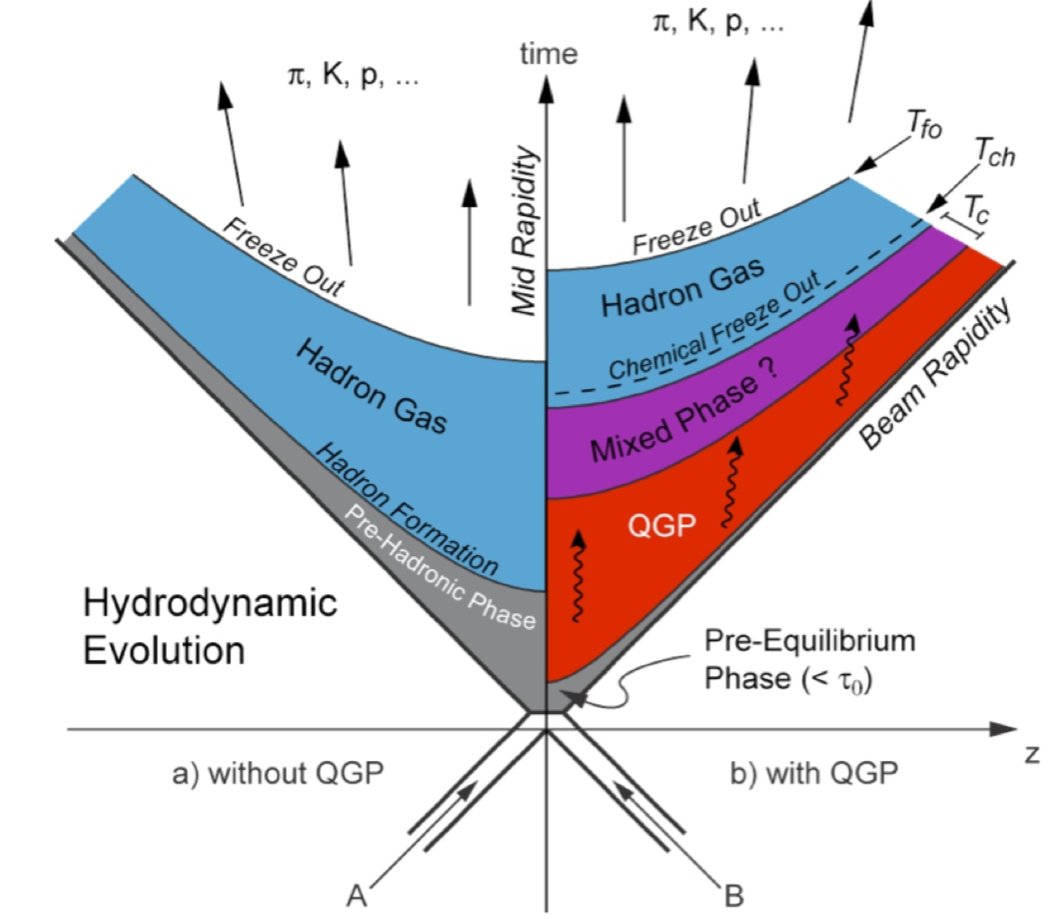
\includegraphics[width=11.0cm]{ppevolution}
\centering
\caption{Comparison of the processes in a proton-proton collision with no medium and a heavy-ion collision with a colored medium stage\cite{PhysRevD.27.140}.}
\label{fig:HeavyIonCollisionvPP}
\end{figure}
\clearpage
}

\subsubsection{Jets and The QGP}

Jets are an excellent probe of the properties of the QGP.  Jets are produced in the earliest stages, before the formation of the QGP, and survive the full evolution of a heavy-ion collision.  As a jet propagates through the QGP, it will lose energy to the medium through a combination of gluon radiation to the colored medium and inelastic scatterings.  These energy loss mechanisms are dependent on the distance a parton travels through the QGP and on the species of the parton.  


\begin{figure}[h]
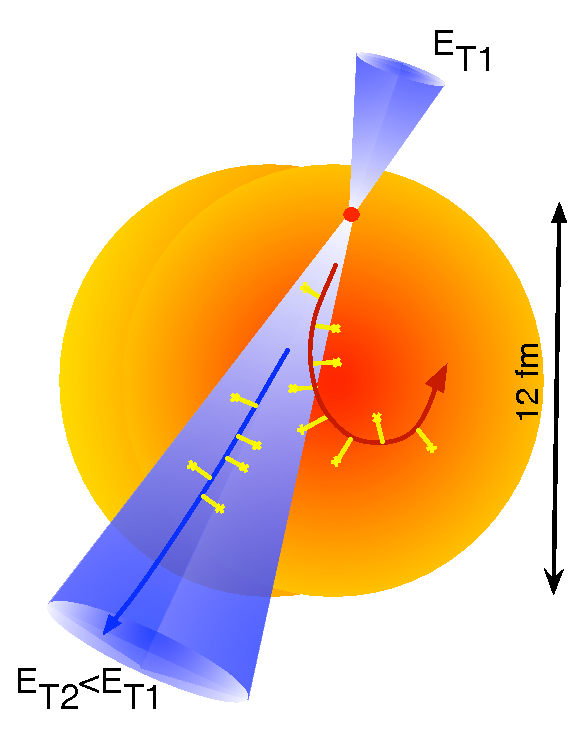
\includegraphics[width=4.5cm]{dijetfig2}
\centering
\caption{Jet energy loss in a QCD medium\cite{Mohanty:2013yca}.}
\label{fig:JetEloss}
\end{figure}

Figure \ref{fig:JetEloss} shows two back-to-back partons undergoing a hard scattering.  Both will fragment into jets, but the first parton with transverse energy, $E_{T1}$, will be subjected to much less energy loss over the second parton due to the first parton only traveling through the outer edge of the QGP.  The species dependent partonic energy loss arises from kinematic constraints to gluon emission from the heaviest of quarks.  This radiation is suppressed at angles smaller than the ratio of the quark mass to its energy and has been dubbed the \textit{Dead-Cone Effect}\cite{Thomas:2004ie}.  Tagging the flavor dependence of jets, either via measuring electrons from semi-leptonic decays or reconstructing the secondary vertex of heavy flavor mesons, has recently shown that energy loss via the Dead-Cone Effect is strongly suppressed with jets containing a charm quark\cite{CAO2018255}.

One way of quantifying the energy loss in a heavy-ion collision is via measurements of the nuclear modification factor, $R_{AA}$,


\begin{equation}
R_{AA} = \frac{1}{N_{binary}} \frac{d^{2}N_{AA}/dp_{T}d\eta}{d^{2}N_{pp}/dp_{T}d\eta}
\label{eq:RAA}
\end{equation}

\noindent
where $N_{binary}$ is the number of nucleon-nucleon collisions and is estimated using a Glauber model\cite{Miller:2007ri} of a nucleus while $d^{2}N_{AA}/dp_{T}d\eta$ and $d^{2}N_{pp}/dp_{T}d\eta$ are the spectra measured in nucleus-nucleus and proton-proton collisions respectively.  $R_{AA}$ may be thought of as asking the question: Does a heavy-ion collision scale as a superposition of $N_{binary}$ nucleon-nucleon collisions?  A $R_{AA}$ value of 1 corresponds to no modification in a heavy ion collision not already present in a proton-proton collision.  The observation of $R_{AA}$ below unity shows a suppression of jets in heavy-ion collisions.  Where does the missing energy go?  This is still a subject for debate and it is not clear whether the energy may propagate outside of the cone radius of the jet or if the energy may become thermalized in the medium.


Figure \ref{fig:JetRAA} shows the nuclear modification factor with R = 0.4 jets in the ATLAS experiment at 5.02 TeV\cite{Aaboud:2018twu}.  The different colored bands in the figure are centralities\footnote{The purple 10 - 20\% band denotes the most central events (i.e. the two colliding nuclei have a low impact parameter and collide nearly head-on), while the 70 - 80\% red band denotes the least central events (i.e. the two colliding nuclei have a high impact parameter and barely graze one another).  An in depth discussion of centrality may be found here\cite{Klochkov_2017}.}

\begin{figure}[h]
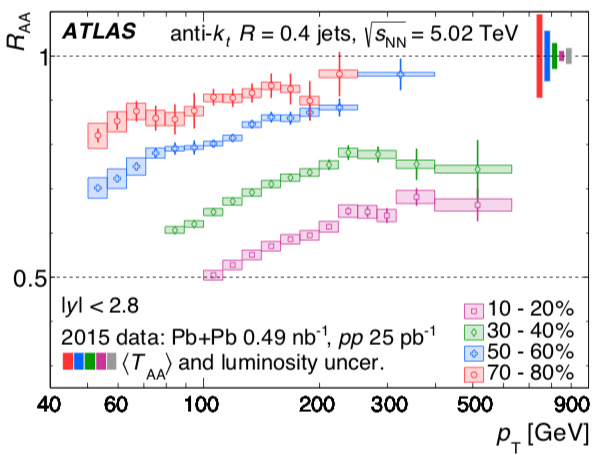
\includegraphics[width=10.0cm]{jetRAA}
\centering
\caption{Jet $R_{AA}$ at 5.02 TeV with the ATLAS experiment\cite{Aaboud:2018twu}.}
\label{fig:JetRAA}
\end{figure}



\subsubsection{Collectivity in Proton-Proton Collisions}
As previously stated a QGP is believed to be absent in proton-proton collisions, thus any signature of a QGP should likewise be absent.  However, one way of quantifying the presence of the QGP is via the Bjorken energy density.  

\begin{equation}
\varepsilon = \frac{1}{\tau A} \frac{dE_{T}}{d \eta}
\label{eq:bjorkenEt}
\end{equation}

\noindent
where A is the transverse area of the nuclei, $\tau$ is the proper time, and $dE_{T}/d \eta$ is the transverse energy per unit psuedorapidity.  It can be shown that  the 150 MeV critical temperature need for the phase transition to the QGP corresponds to ~ 1 - 3 GeV/$fm^{3}$ energy density.  The quantity $dE_{T}/d \eta$ can be related to the mean transverse momentum $<p_{T}>$ and particle multiplictiy\footnote{Multiplicity is defined as the number of particles per event} per unity psuedorapidity as:

\begin{equation}
\frac{dE_{t}}{d \eta}  \approx  <p_{T}> \frac{dN}{d\eta}
\label{eq:Et}
\end{equation}

where $ <p_{T} >$ is the mean transverse momentum and $dN/d\eta$ is the particle multiplicity per unit psuedorapidity.  This suggests that in very high multiplicity proton-proton events signatures of the QGP may be present.  Although suppression has never been observed in high multiplicity proton-proton collisions, physicists have recently measured azimuthal correlations in such systems\cite{Nagle:2018nvi}.  This gives a `hint' that flow may be present in high multiplicity proton collisions.  CMS presented results in proton-proton collisions at 13 TeV using soft-particles, $p_{T} \leq\,$ 2 GeV/\textit{c}, consistent with hydrodynamical predictions\cite{ZHAO2018495}. These results have opened new debates and questions into the very nature of the QGP.  Measuring jets to high accuracy over a wide kinematic range is important because it serves as a baseline measurement for the inducing the QGP properties in heavy-ion collisions.  This will be explored in more detail throughout the rest of this thesis.
    \chapter{The LHC and ALICE}\label{ch:alice}

\section{Overview of The LHC}\label{sec:LHC}
The Large Hadron Collider (LHC)\cite{doi:10.1142/S0217751X13300354} is a circular particle accelerator located on the Franco-Swiss border near the city of Geneva.  It is operated by the European Organization for Nuclear Research (CERN) and has carried out proton-proton (pp), lead-proton (pPb), and lead-lead (PbPb) collisions at center of mass energies of  0.9-14 TeV, 5.0 TeV, and 2.76-5.5 TeV, respectively.  The LHC is approximately 17 miles in circumference and is located 200 meters underground, inside the old accelerator tunnel used by the Large Electron-Positron\cite{Taylor:2017edx} collider of the 1980's.  There are over 8000 physicists and engineers making up the four main experiments at the LHC: ATLAS\cite{Aad:2008zzm}, CMS\cite{Chatrchyan:2008aa}, LHCb\cite{Alves:2008zz}, and ALICE\cite{Aamodt:2008zz}.   Numerous physics results have been published, with the most famous being the discovery of the Higgs boson in 2012\cite{Chatrchyan:2012xdj}\cite{Aad:2012tfa}.

\begin{figure}[h]
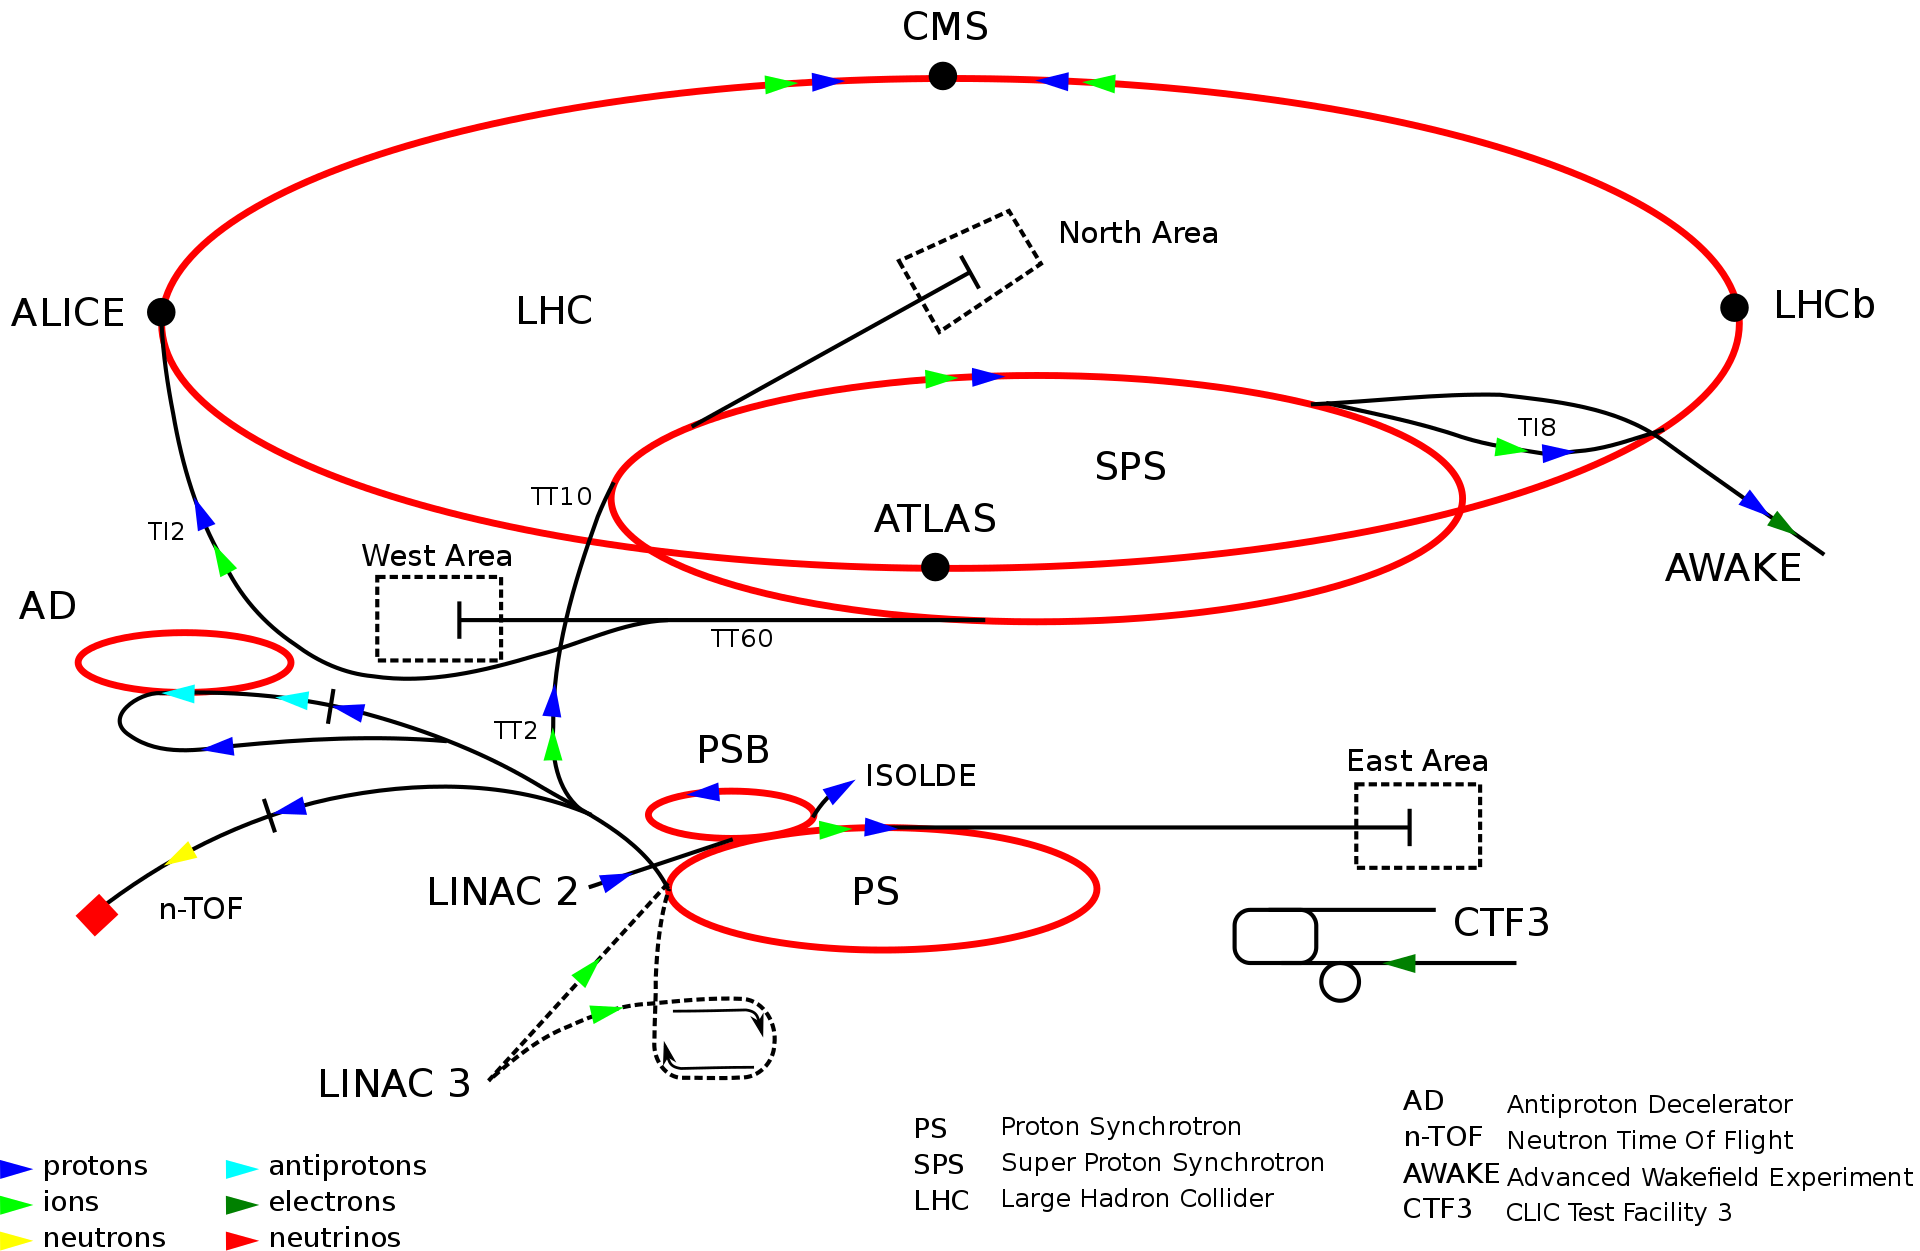
\includegraphics[width=15.0cm]{1920px-Cern-accelerator-complex}
\centering
\caption{LHC accelerator complex.  The four main experiments are shown in their relative locations\cite{Mobs:2197559}.}
\label{fig:AccComp}
\end{figure}

Figure \ref{fig:AccComp} shows a schematic of the LHC along with the pre-accelerators that help to accelerate protons and ions to their final energies before a collision at one of the four experimental interaction points (IP).  Protons are injected into the LHC in groups called `bunches'.  Every bunch is comprised of about 120 billion protons with about 50 nanoseconds between the arrival of the next bunch.  The bunch scheme during the heavy-ion run is reduced to 200 nanoseconds due to the high multiplicity of the events and additional computational resources needed. 

\subsubsection{LHC Operations}
The LHC first attempted particle collisions in September of 2008.  The initial ramping up of the super conducting magnets led to mechanical failure of the helium pipes inside of the LHC beam line.  This fault caused the LHC to remain shut down for over a year while the accelerator was repaired and new safety procedures were implemented. The first successful collisions occurred in 2009 with proton collisions at a reduced energy of 0.9 TeV.  2010 marked the beginning of a new era in the high energy frontier with proton collisions at a record setting 7 TeV.  The only other major fault that has occurred was in the summer of 2016. A stone marten chewed through a high voltage line in a power transformer on a ground level building at the LHC.  The LHC went offline for about a week while repairs occurred and quickly resumed the physics program.  Unfortunately, the marten did not survive.

The typical operating year at the LHC allows for any repairs or upgrades on the experiments to be performed during the offline period for the first few months.  After the offline period, the proton physics program begins and lasts until approximately mid-November.  The heavy-ion program begins after the proton physics run and lasts until the first week of December, after which the LHC shuts down for the remainder of the year.  

From 2014 until early 2015 the LHC was shutdown for major renovations and upgrades to the accelerator and a number of sub-detectors on each experiment. This was known as long shutdown 1 (LS1).  Since the end of 2018, the LHC has been in another long shutdown (LS2), which aims at upgrading the accelerator to a high luminosity, Hi-Lumi.  This will be discussed in detail along with the upgrades to ALICE in Chapter \ref{ch:tpcu}.

\subsubsection{LHC Accelerator Complex}\label{sec:LHCop}
The LHC accelerator complex is a succession of particle accelerators that increase the energy of particles before they are injected into the next accelerator.  Hydrogen atoms are first passed through a high voltage environment that strips any electrons from around the proton.  Once the protons are stripped of their electrons, they are injected into the linear accelerator (LINAC).  The LINAC uses radio frequency cavities to accelerate particles to 50 MeV before they enter the first circular accelerator the Proton Synchrotron (PS).  The PS begins to focus the protons into bunches and further accelerates them to 1.4 GeV before the the beam enters the Super Proton Synchrotron (SPS).  The SPS accelerates the particles to 450 GeV.  The beam is then injected into the LHC and accelerated to the final collision energy.  Afterwards the beam gets `squeezed', or tightly focused, with a series of quadrupole magnets.  The final step is to `adjust'  the beam to overlap with the counter-rotating beam at the four interaction point (IP) were the main LHC experiments are located.  Once the adjust phase is completed, collisions will occur at each experiment and data  collection begins.  This entire process from stripping the electrons to collisions in each IP takes 20 minutes.

In order for the beam parameters to be maintained in the LHC, numerous dipole and quadrupole magnets are used to accelerate, focus, and bend the particle beams.  The magnets use a superconducting niobium-titanium alloy that is maintained at an operating temperature of 1.9 K using helium-4.  Upgrading these magnets is one of the major goals during LS2 as part of the Hi-Lumi upgrade of the LHC\cite{Fabjan:2011jb}.


\section{The ALICE Experiment}
A Large Ion Collider Experiment (ALICE) is a general purpose detector that covers a solid angle of 4$ \pi$ around the IP.  It is 26 m long, 16 m high, 16 m wide, and weighs approximately 10,000 tons\cite{Fabjan:2011jb}.  Like many other large scale detectors, ALICE is made up of 18 sub-detectors that perform tracking, particle identification (PID), timing, vertex reconstruction, and calorimetry.  


Figure \ref{fig:alice} shows the ALICE detector with human figures to set the scale.  Figure \ref{fig:ITS} shows the area closest to the interaction point with the TZERO, VZERO, Inner Tracking System and Forward Multiplicity Detector.  These detectors give basic information on the collision such as vertex location, centrality, and timing.   Further out from the central region are a number of tracking detectors, like the Time Projection Chamber and Time-of-Flight detectors, which focus on  measuring charged particle momentum and PID.  Next are the calorimeters that measure particle and jet energies, such as the Electromagnetic Calorimeter, Photon Spectrometer, and  Dijet Calorimeter.  All of these sub-detectors are housed in the L3 magnet, seen as the red octagon in Figure \ref{fig:alice}.   The L3 magnet provides an approximately uniform magnetic field of 0.5 T over the central area of ALICE and helps ensure the high PID performance ALICE has over a wide kinematic region\cite{Gligorov:2018vkc}.  At high rapidity, there is a muon tracker and trigger for muon identification.  The following sections give a more detailed discussion of the sub-detectors used for this analysis

\afterpage{%
\begin{figure}[h!]
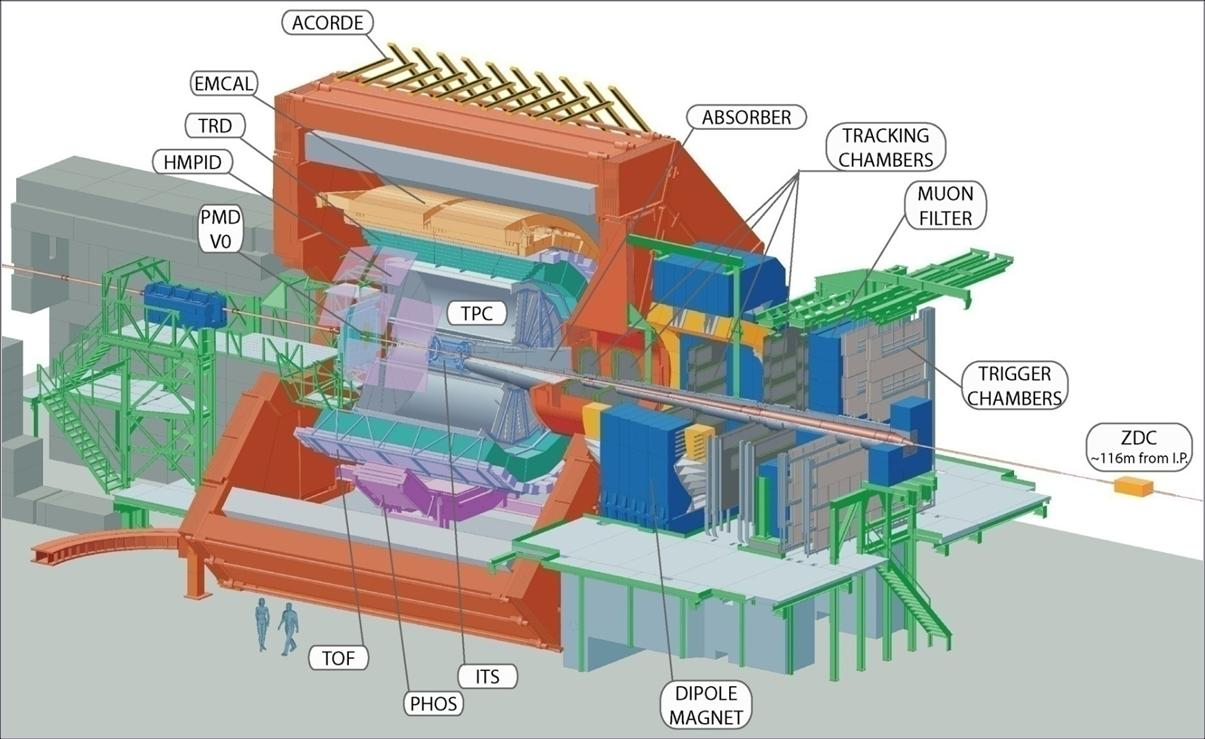
\includegraphics[width=\linewidth]{ALICE-event-b}
\centering
\caption{The ALICE Detector at CERN\cite{Alberico:2011zy}.}
 \label{fig:alice}
\end{figure}

\begin{figure}[h!]
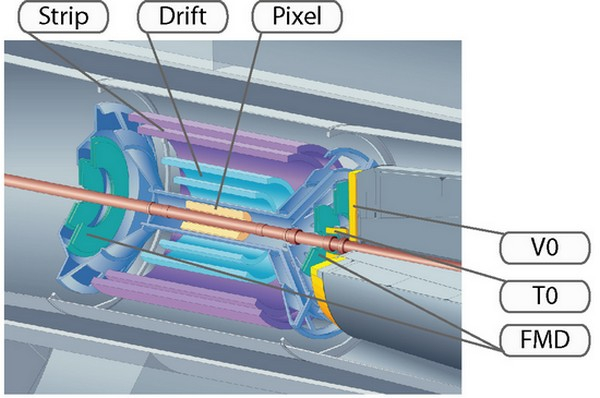
\includegraphics[width=10cm]{ITS}
\centering
\caption{ALICE tracker, multiplicity, timing, and vertex detectors located near the interaction point\cite{Alberico:2011zy}.}
 \label{fig:ITS}
\end{figure}
\clearpage
}

\subsubsection{TZERO}
The TZERO (T0)\cite{Bondila:2005xy} detector is a double layer Cherenkov counter located at 70 cm (T0A) and 370 cm (T0B) from the IP.  The T0 functions as a trigger and timing detector that determines the precise moment in time at which an event `starts' in the ALICE detector.  The timing information from the T0 is fed to other sub-detectors, like the Time-of-Flight and Time Projection Chamber detector, which is used for track reconstruction. in the case of the Time Projection Chamber  The T0 also gives feedback on the target luminosity of the ALICE experiment to the LHC operations center.  

\subsubsection{VZERO}
The VZERO (V0)\cite{Abbas:2013taa} detector is a double layer scintillator array and similar to the T0 is asymmetrically placed at a distance of 86 cm (V0A) and 329 cm (V0C) away from the primary IP.  It provides the `minimum bias' (Min Bias)\footnote{A Min Bias event is unsurprisingly defined as an event with the least amount of bias possible.  Events recorded with a Min Bias trigger attempt to not artificially prefer either diffractive or non-diffractive processes over one another\cite{Field:2011iq}.} trigger information for events and centrality information during the heavy-ion run.   Centrality\footnote{Centrality (c) is an estimation of the impact parameter (b) between the two colliding nuclei.  It is proportional to the cross-section and is given as $c = \frac{1}{\sigma_{inel}} \int^{b}_{0} db \frac{d\sigma}{db}$} is determined by measuring the multiplicity amplitude from the V0 and fitting these results to a Glauber\footnote{The Glauber model treats the nucleons composing a nucleus as hard shells, more can be found here \cite{Loizides:2016djv}.} distribution.  The V0 is also capable of precision measurements of the target luminosity in the ALICE detector.


\subsubsection{Inner Tracking System}\label{sec:its}
The Inner Tracking System (ITS)\cite{BEOLE20121062} is six layers of solid state silicon detectors.  Closest to the beam line are two layers of Silicon Pixel Detectors.  The next two layers are Silicon Drift Detectors and furthest from the beam line are two layers of Silicon Strip Detectors.  The main purpose of the ITS is to perform momentum measurements, PID, and vertex reconstruction of charged tracks.  PID\footnote{See Appendix \ref{ref:pid}} is performed by measuring the ionization energy, $\frac{dE}{dx}$, of charged particles as they traverse the detector\cite{Adam:2016acv}.  The ITS has a spatial resolution of 100 $\mu m$.  This allows for measurements of short lived hadrons by reconstructing secondary vertices, which is useful in measuring hadrons containing heavy quarks, bottom and charm.


%TPC

\subsubsection{Time Projection Chamber}\label{sec:tpc}

\begin{figure}[h]
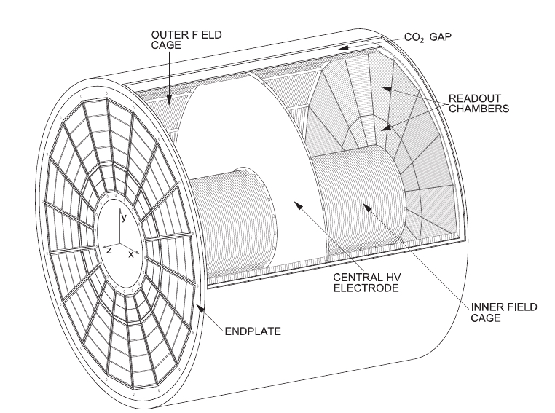
\includegraphics[width=12.0cm]{alice-tpc-schematic}
\centering
\caption{The ALICE Time Projection Chamber\cite{2010NIMPA.622..316A}.}
\label{fig:TPC}
\end{figure}

The Time Projection Chamber (TPC)\cite{2010NIMPA.622..316A} is a gaseous charged particle tracker and the largest of its kind in the world.  The TPC has full azimuthal coverage, a pseudorapidity acceptance of $ \left | \eta \right | \leq 0.7$, and a volume of 93 $m^{2}$.  Figure \ref{fig:TPC} shows a schematic of the TPC.  As charged particles traverse the drift volume of the TPC, they ionize the gas inside\footnote{The TPC has operated with $Ne-CO_{2}$ (90-10) and $Ar-CO_{2}$ (90-10) gas mixtures in the past}.  A central cathode in the TPC wth a voltage of 100 kV induces a uniform electric field of 400 V/m along the beam axis throughout the drift volume.  Ionized electrons will drift down to the cylindrical endcaps of the TPC where the read-out chambers (ROC) are located.  There are 18 ROCs on each side of the TPC which are further broken into an Inner Read Out Chamber (IROC) and an Outer Read Out Chamber (OROC).  

\subsubsection{The TPC Readout}\label{sec:tpcread}

\begin{figure}[h]
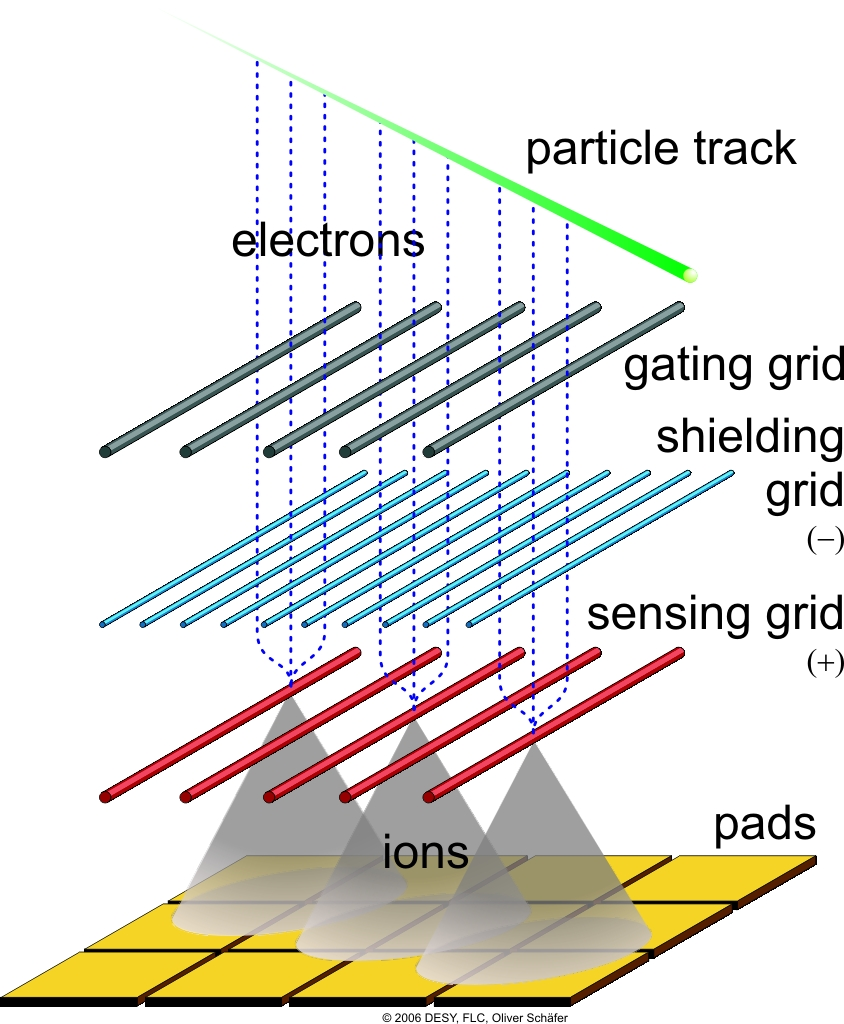
\includegraphics[width=9.0cm]{Wirereadout_eng}
\centering
\caption{The TPC readout region\cite{diener}.}
\label{fig:TPCreadout}
\end{figure}

The TPC incorporates a Multi-Wire Proportional Chamber (MWPC) design for amplification and copper pads for readout\footnote{There are 72 MWPCs and 500K copper pads in the ALICE TPC}. Ionized electrons created from charged particles take approximately 100 $\mu s$ to move from the drift volume to the readout region.  Once these electrons enter the readout region, they will undergo an amplification process with the MWPC, seen as the sensing grid wires in Figure \ref{fig:TPCreadout}.  This amplification process will turn the few dozen ionizated electrons generated from a charged particle into thousands of amplified electrons that are sensed by the cooper pads and read from the front-end electronics(FEE).  

Amplification using MWPCs has the disadvantage of creating thousands of ions known as `backflow ions' that can move back into the drift volume of the TPC.  The presence of backflow ions in the drift volume of the TPC will cause distortions in the uniform electric field of the TPC.  These distortions are known as `space-charge' distortions and will compromise the physics performance of the TPC.  In order to minimize the space-charge distortions, the TPC incorporates a gating grid\cite{Tangwancharoen:2016dqs}.  Once an event is detected in the readout electronics of the TPC, a high voltage is induced on the gating grid.  This will capture any backflow ions moving from the amplification region to the drift volume.  When engaged, the gating grid introduces a dead time as any ionization electrons from new events occurring in ALICE will also get captured.  The current configuration of the gating grid is designed to engage for 300 $\mu s$ after an event is first detected.  This has been shown to absorb approximately 99\% of the backflow ions created while preserving the TPC physics performance.  The dead time due to the gating grid along with the drift time for charged particles in the TPC limits the readout to 3.5 kHz.  Upgrading the triggered operation of the current TPC to a continuous readout for the Hi-Lumi upgrade of the LHC will be discussed in detail in Chapter \ref{ch:tpcu}.

\subsubsection{TPC Performance}\label{sec:tpcper}

In order to reconstruct the trajectory of a particle, an iterative process known as a Kalman filter approach is used.  The x, y coordinates, which are perpendicular to the beamline, are determined via the signal induced on the copper pads.  The z component, which is parallel to the beamline, is reconstructed using the timing information from the T0.  

\begin{figure}[h]
   \centering
      \subfloat[TPC momentum resolution]{\label{fig:figure-TPCb}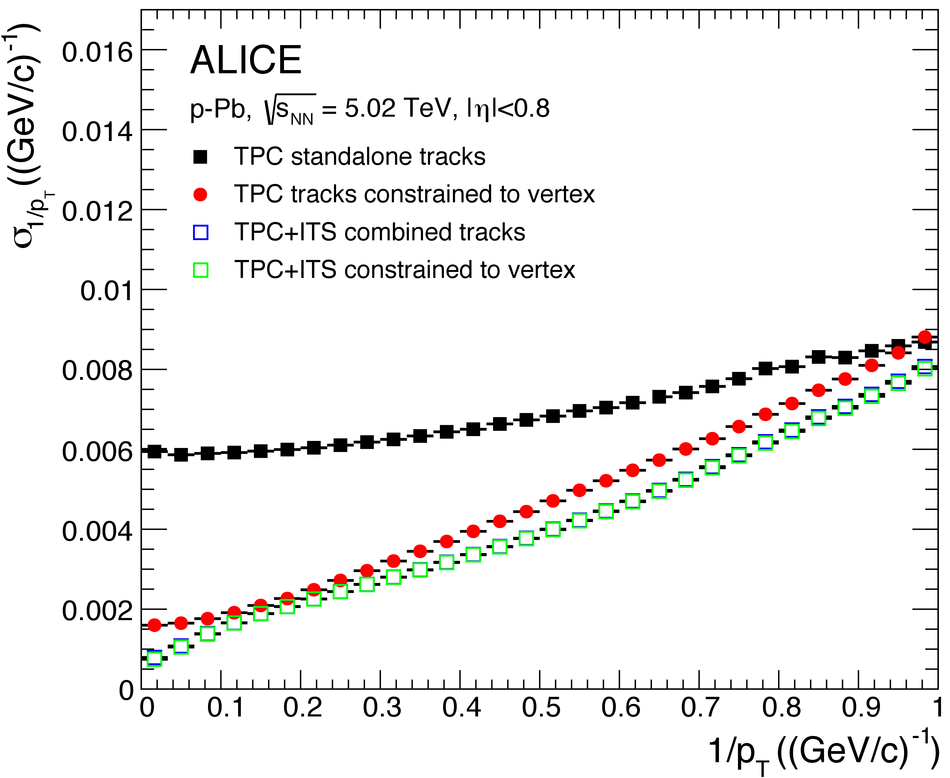
\includegraphics[width=3.0in]
     {PTresolution_vs_1Pt_pPb_2013_PerfPaper-8441}}
   \subfloat[ITS-TPC track matching efficiency]{\label{fig:trk-match}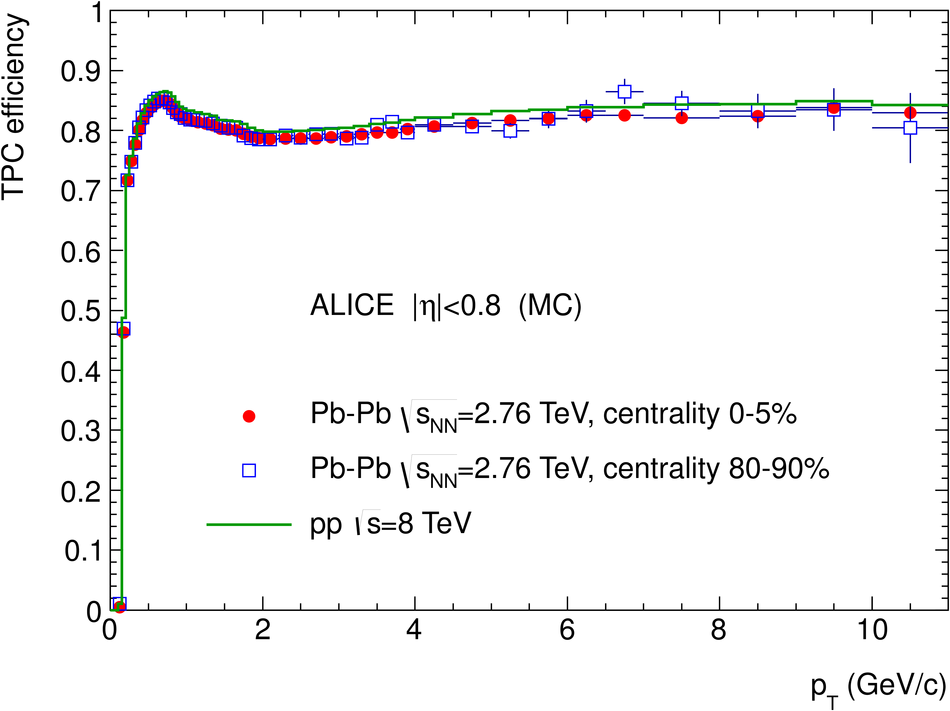
\includegraphics[width=3.0in]
     {tpc_abseff-8423}}
   \caption{TPC momentum and tracking resolution\cite{Abelev:2014ffa}.}
   \label{fig:multipart-TPC}
\end{figure}


The TPC has excellent momentum resolution between 150 MeV/\textit{c} to 100 GeV/\textit{c}\cite{LIPPMANN2012434}.  Figure \ref{fig:figure-TPCb} shows the inverse momentum resolution as being below 5\% in black.  The inverse momentum resolution was further improved to below 0.5\% over the full kinematic range by matching TPC tracks to ITS tracks and constraining those tracks to originating from the primary vertex region, red and green respectively.  The total efficiency between ITS tracks to TPC tracks is stable at about 80\%, as seen in Figure \ref{fig:trk-match}.



%EMCAL

\subsubsection{Electromagnetic Calorimeter}
The Electromagnetic Calorimeter (EMCal)\cite{1742-6596-293-1-012043} is a lead based sampling calorimeter located at a radius of 4.5 meters from the beam pipe.  It covers a pseudorapidity of $ \left | \eta \right | \leq 0.7$ and has azimuthal coverage of $ \Delta \phi = 107 \deg$.

\begin{figure}[h]
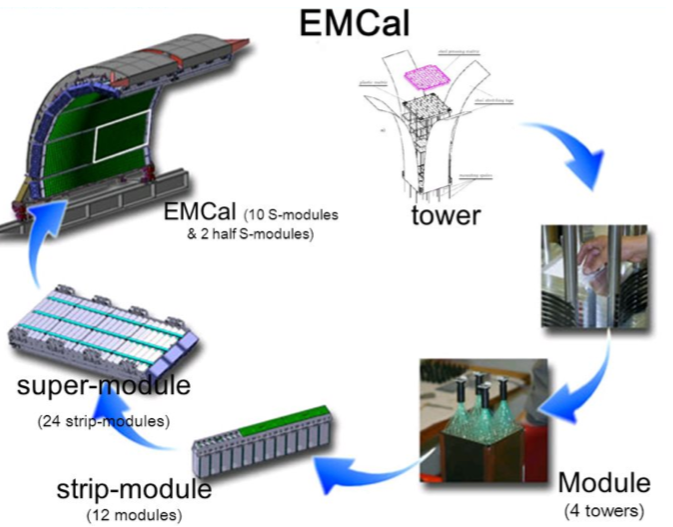
\includegraphics[width=12.0cm]{ALICEEMCAL}
\centering
\caption{ALICE EMCal along with super modules, tower strips, and towers\cite{1742-6596-110-3-032006}.}
\label{fig:EMCal}
\end{figure}


Figure \ref{fig:EMCal} shows the layout of the EMCal.  The smallest element of the EMCal is the `tower'\footnote{There are 12K towers in the EMCal}.  The tower serves as the readout and is made up of several layers of alternating scintillator and Pb-absorber.  Particles that interact via the electromagnetic force initiate a shower in the absorber material in the tower.  This electromagnetic shower induces light in the scintillator  to accumulate in the avalanche photodiodes in proportion to the particle's energy.  A `module' is an array of four towers that share readout electronics.  Twelve modules are placed in a single strip that provides support to the structure.  The largest component of the EMCal is the super-module, consisting of 1,100 towers,  which serves as the mounting structure to the ALICE detector.  The super-modules span a 20 degree angle in azimuth and ALICE currently has 10 full sized super-modlues and two 1/3 size super modules.  A second calorimeter was installed in 2015, the Dijet Calorimeter(DCAL), and allows for back-to-back jet measurements.


\subsubsection{EMCal Performance}
As particles enter the EMCal they initiate an electromagnetic shower.  The shower of electromagnetic particles spans several neighboring towers, these towers are grouped together into `clusters' and the Analog-To-Digital Conversion signal from the clusters corresponds to the energy deposited by the particle.  The EMCal was designed so that photons and electrons will fully shower inside of the tower region and thus fully deposit their energy.  Hadrons on the other hand will usually punch through the EMCal and only deposit a small fraction of their energy. 

 PID can be performed using the EMCal via track-cluster matching from the TPC.  TPC tracks are geometrically matched to the centroid of a cluster and if no track is matched, the cluster originated from a photon. If a track is matched, then the ratio of E/P, the energy of a matched cluster to the momentum of a TPC track, can be used to separate electrons from hadrons.

The energy resolution of the EMCal follows the form seen in Equation \ref{eq:emcalres}



\begin{equation}
\frac{\sigma}{E} = \sqrt{ A^{2} + \frac{B^{2}}{E} + \frac{C^{2}}{E^{2}}  }
\label{eq:emcalres}
\end{equation}

\noindent
where E is the cluster energy, A characterizes stochastic fluctuations such as photon collection efficiency, B is a function of the systematic effects such as detector non-uniformity, and C is a function of the noise in the Front-End Electronics (FEE). 

\begin{figure}[h]
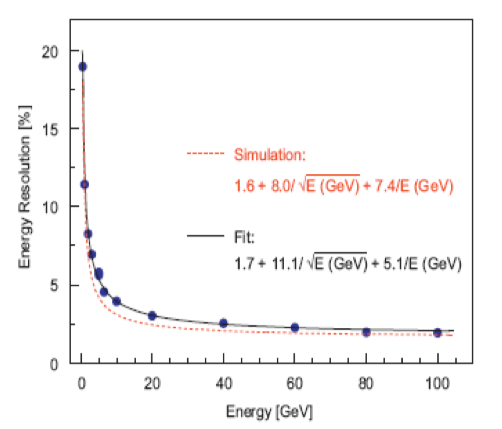
\includegraphics[width=11.0cm]{Alice-EMCal-Performance}
\centering
\caption{Energy resolution in the EMCal measured in a 2007 test beam at CERN (blue) compared to GEANT3 simulations of the EMCal (orange), fits for the parameters A, B, and C are also shown\cite{Abeysekara:2010ze}.}
\label{fig:EMCalres}
\end{figure}


As seen in Figure \ref{fig:EMCalres}, excellent agreement exits between the measured performance of the EMCal compared to simulations in a kinematic range between 10 GeV - 100 GeV and the resolution improves as the particle energy increases.  The stochastic term, A, is the largest source of uncertainty in the energy resolution in the EMCal.  Unlike the TPC, the resolution improves at high-$p_{t}$ making the EMCal ideal for measuring high energy particles and jets.


\subsubsection{EMCal Trigger}


Due to the high luminosity in the LHC, only a small fraction of events may be recorded to disk for later analysis.  ALICE employs a variety of triggers to record events that have the highest value for performing quality physics analysis.  The EMCal can trigger on events in order to increase the effective sample size for high-$p_{T}$ jets, photons, and electrons.  The two main triggers\cite{bourrion2010level}\cite{bourrion2013alice} for the EMCal are a jet trigger and a gamma trigger.  The gamma trigger is comprised of a 4x4 patch of EMCal towers, while the jet trigger is a 16x16 patch of towers.  Once the gamma trigger has surpassed a minimum energy threshold of 5 GeV\cite{Kral2012261} the event is tagged as a gamma event and the patch location is recorded.  EMCal jet triggered events have an energy threshold of 20 GeV and are similarly tagged and recorded.  The 5 GeV and 20 GeV thresholds used to fire the EMCal triggers are not fixed and the values quoted are specific to the 2012 8 TeV data set. 

\begin{figure}[h]
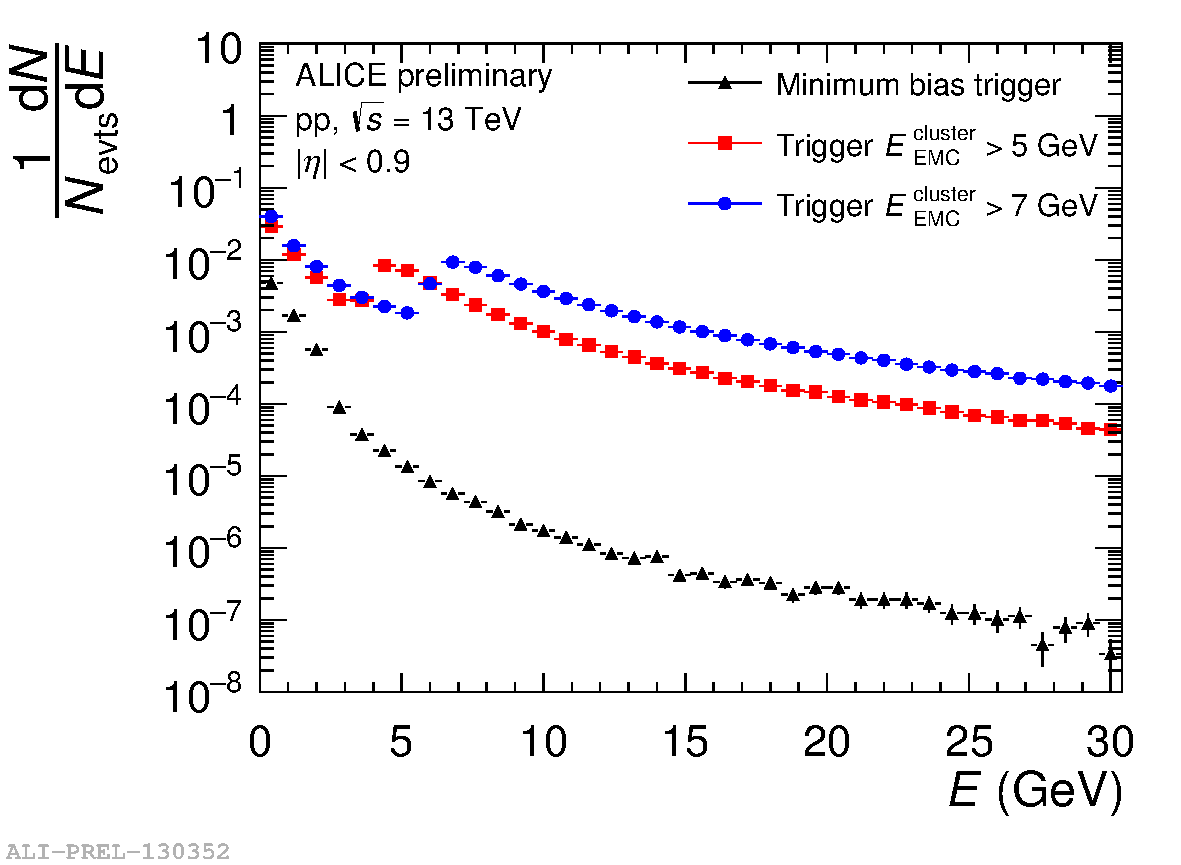
\includegraphics[width=12.0cm]{2017-Jul-05-Ecluster_emcal_alice_style}
\centering
\caption{Cluster Spectra from the ALICE EMCal.  MinBias is shown in black while the red and blue points show the spectra using the gamma trigger at two energy thresholds\cite{Jahnke:2018mrq}.}
\label{fig:EMCalSpectra}
\end{figure}

Figure \ref{fig:EMCalSpectra} shows the spectra from clusters measured in the EMCal using MinBias data in black and the gamma trigger from the EMCal set to two thresholds, 5 GeV and 7 GeV.  Recording the events that satisfy the EMCal triggers introduces a bias towards high-$p_{T}$ processes.  By using events that had an EMCal trigger, we can extend the kinematic range of an inclusive jet measurement, as seen in Figure \ref{fig:EMCalSpectra}.  In order to account for this bias it is necessary to calculate a trigger efficiency by comparing spectra from inclusive jets recorded using the MinBias trigger to the spectra generated from the EMCal triggers in the 8 TeV data set.  The calculation of the trigger efficiency will be discussed in depth in Chapter \ref{ch:analysis}.
    \chapter{The ALICE TPC Upgrade} \label{ch:tpcu}

From 2014 until 2018, I worked on the upgrade of the TPC to a continuous readout.  This includes working on a test beam in 2014 for a prototype Read-Out Chamber (ROCs) using Micropattern Gaseous Detectors (MPGD) over the current Multi-Wire Proportional Chamber (MWPC) design.  Once a final design for the new ROCs was chosen the production of the new Inner Read-Out Chambers (IROCs) using a stack of four Gaseous Electron Multiplier (GEM) foils took place at the University of Tennessee.  During this period I assembled 49 new IROCs.  In 2018, I traveled to Yale University and CERN to help with quality assurance of the IROCs built at Tennessee.


\subsection{Physics Motivation}
After the 2018 heavy-ion run ends, the LHC will begin the second long shutdown (LS2) and upgrade to the High Luminosity LHC (Hi-Lumi LHC)\cite{Apollinari:2015bam} which was briefly mentioned in section \ref{sec:LHC}.  The goal of the LHC upgrade is to move into an era of high precision measurements of rare QCD processes and increase the production of soft probes.  Once the upgrade is complete the expected event rate in ALICE will be 50 kHz in MinBias PbPb collisions.  This will lead to a factor of x100 increase in MinBias data and a factor of x10 increase in high-$p_{T}$ triggered data recorded by ALICE.

The ALICE experiment has focused on probing the thermodynamic properties of the QGP in the past.  The increase in event rate expected from the Hi-Lumi LHC would open new ways to probe the QGP including\cite{Abelev:1475243}:

\begin{itemize}
\item[-] Increasing the production of jets and allowing separation of jet measurements based on the flavor of the initial parton.
\item[-] Studying the production mechanisms of light-nuclei, antihyper-nuclei, and other exotic hadrons.
\item[-] Probing the initial state temperature and equation of state of the QGP by measuring low-mass dileptons that originate from the earliest stages of a heavy-ion collision.
\item[-] Increase the yields of heavy-flavor mesons reconstructed via the secondary-vertices. 
\end{itemize}

\noindent
In order to do this ALICE will implement a number of upgrades \cite{1742-6596-589-1-012014} during the shutdown that include:

\begin{itemize}
\item Replacing the V0 and T0 detectors with a combined detector, called the Forward Interaction Trigger (FIT)\cite{1742-6596-798-1-012186}.
\item Improving the ITS and Muon Tracker spatial resolution by using  Monolithic Active Pixel Sensors (MAPS)\cite{Abelev:1625842}\cite{CERN-LHCC-2015-001}.
\item Removing the 400 nanosecond dead time associated with the TPC and upgrade the FEE cards to handle the increase in data bandwidth\cite{Abelev:1475243}.
\item New Online/Offline ($O^{2}$) data processing architecture\cite{Buncic:2011297}.
\end{itemize}

\noindent
Leptons weakly couple to the QGP\cite{Ryblewski:2015sha} and by studying these the initial states in heavy ion collisions may be probed\cite{Mauricio:2007vz}.  Figure  \ref{fig:lowmassdilep} shows a simulation of the mass spectra for dileptons between 0 GeV/\textit{c} - 1 GeV/\textit{c} using the current ALICE central detectors with tight kinematic cuts (left).  The yields that are quantifiable do not allow for the separation of leptons originating from the QGP from those originating from background sources.  After the increase in event rate and the upgraded ITS with improved tracking capabilities, measuring the low-mass dileptons that interacted with the QGP will be possible as shown on the right of Figure \ref{fig:lowmassdilep}. 

\begin{figure}[h]
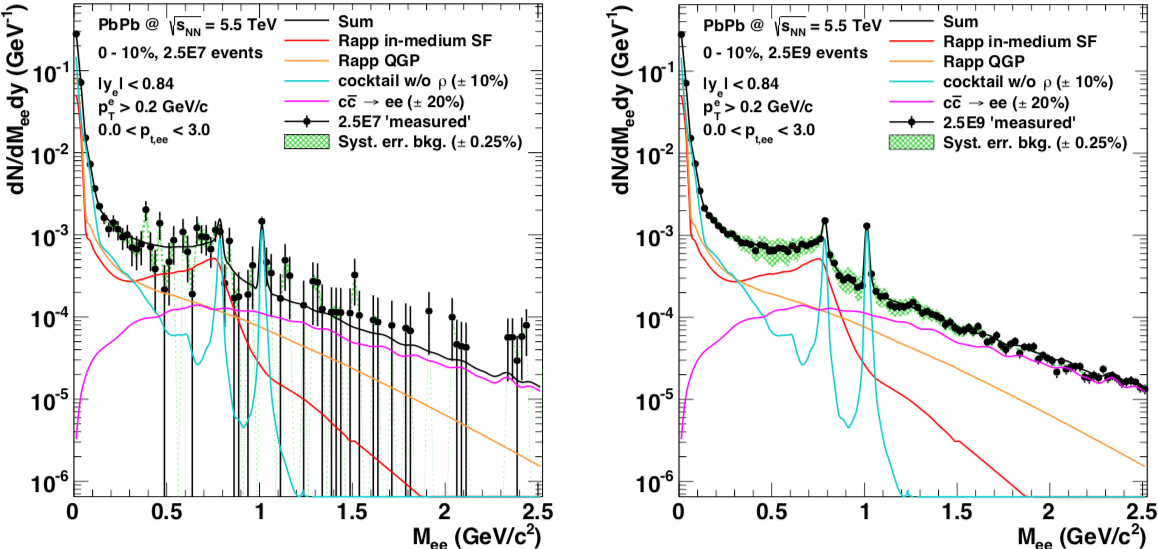
\includegraphics[width=\linewidth]{dilepton-mass}
\centering
\caption{Simulation of the invariant  mass spectra for dileptons in a typical heavy-ion run with current ALICE performance (left) and after upgrade of ALICE for Run-3 (right) in PbPb at $\sqrt{s_{NN}}$ = 5.5 TeV.  The dilepton yields originating from the QGP are shown (red and orange), along with background contributions from light-hadrons (blue), and charm (magenta)\cite{Abelev:1475243}.}
\label{fig:lowmassdilep}
\end{figure}

\noindent
The TPC used in the ALICE experiment along with the readout was discussed in section \ref{sec:tpc}.  The ALICE collaboration first proposed an upgrade of the TPC in 2012 with a Letter of Intent (LoI)\cite{Abelev:1475243}.  A Technical Design Report(TDR)\cite{CERN-LHCC-2013-020} was published in 2013 with an initial design overview.  An addendum to the TDR\cite{CERN-LHCC-2015-002} was published in 2015 after the performance of prototype ROCs was measured on a test beam at CERN in 2014.  The overall goals of the TPC upgrade are to continuously readout events in the high luminosity environment expected after LS2, to minimize the accumulation of space-charge distortions in the drift field, and to maintain the PID and tracking performance of the current TPC.


\subsection{Gaseous Electron Multiplier Foils}
Gaseous Electron Multiplier (GEM) Foils were first proposed by CERN physicist Fabio Sauli in 1997\cite{Sauli:1997qp}.  GEMs belong to a new form of detector technology known as Micropattern Gaseous Detectors\cite{Titov:2013hmq} that use microelectronic or chemical etching techniques to print a readout structure onto a material surface.

\begin{figure}[h]
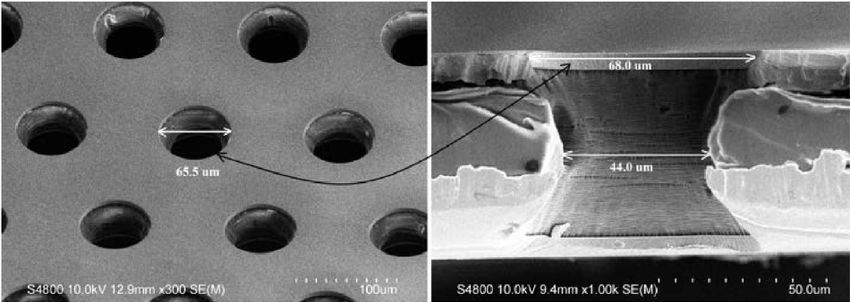
\includegraphics[width=14.0cm]{Scanning-electron-microscopy-image-of-GEM-foil-top-view-left-and-cross-section-right}
\centering
\caption{Scanning electron microscope image of a GEM foil from top (left) and profile (right)\cite{Brucken:2017qjy}.}
\label{fig:GEMpic}
\end{figure}

\noindent
GEM foils are a Kapton sheet, typically 50 $\mu m$ thick, with a thin copper coat on both sides of the surface.  A weak acid and stencil are used to chemically etch holes throughout the foil.  Typically, the holes are between 10 $\mu m$ - 100 $\mu m$ in diameter and between 100 $\mu m$ - 300 $\mu m$ in pitch as seen in Figure \ref{fig:GEMpic}.  A few hundred volts is applied to each of the copper surfaces of the GEM foil causing a strong electric field to be induced in the GEM holes\footnote{The electric field is on the order of 10 kV/cm}.  

When a ionization electron from a track enters a GEM hole it will cause an avalanche of amplification electrons and ions to be produced similar to MWPCs.  Due to the high voltage and strong electric fields around the GEM foil, any back flow ions created from the avalanche will get absorbed by the copper surfaces on the GEM foil, as seen in Figure \ref{fig:GEMefield}.
\begin{figure}[h]
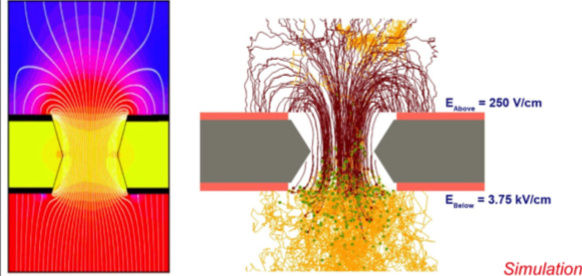
\includegraphics[width=14.0cm]{ALICEGEMSIMULATION}
\centering
\caption{Profile of GEM with electric-field lines and gradients (left).  Simulation of an ionization electron (yellow line) entering a GEM from a drift volume, amplification electrons (green dots, yellow lines) and back flow ions (red lines) are created (right)\cite{Bhattacharya:2017yaj}.}
\label{fig:GEMefield}
\end{figure}

\noindent
The configuration of the pitch and size holes ion a GEM foil is directly correlated to the amplification properties and ability to capture back flow ions.  GEMS with larger holes or shorter pitch between the holes will have more amplification but will also be more ineffective at capturing ions.  Likewise, GEMs with shorter holes or larger pitch will have better ion capture abilities yet worse amplification properties.  By stacking multiple GEMs on top of one another it is possible to maximize the amplification properties and minimize the backflow. 

Creating GEMs with a uniform hole distribution and stacking them in a consistent manner in order to minimize the overlap of holes from one layer to another restricted them to small prototypes and impeded their use on large experiments.  Around 2010 two methods were developed, the single-mask technique\cite{0960-1317-17-8-021} and the NS2 assembly\cite{1748-0221-12-06-C06036}, which allowed for a systematic way of etching holes and stretching GEMs so they could be properly aligned.  These methods allowed for GEMs to become a viable amplification device for large experiments.  As of 2018 the TOTEM, COMPASS, ATLAS, and LHCb experiments have all incorporated GEMs in their trackers and future colliders, such as the Electron-Ion Collider (EIC), plan on using them\cite{SAULI20162}.


\subsection{Research and Development}

Initially, it was decided that the new ROCs would incorporate a stack of three GEMs with a hole geometry similar to the one incorporated on the LHCb experiments\cite{Santimaria:1690550} tracking detector.  This gave the ALICE TPC upgrade a starting point to bench mark performance for the upgrade as well as the opportunity to use experts in GEM technology already present at CERN.  The first phase of the R\&D involved simulating the performance of the LHCb 3-GEM stack in the high event rate environment expected  after the Hi-Lumi LHC upgrade using a the software package called Garfield++, which is a GEANT4 add-on package built to simulate MPGDs.  It was quickly observed from the simulations that a 3-GEM stack would be insufficient in maintaining the performance needed for the TPC while minimizing the ion back flow.  An additional layer of GEM was added to the 3-GEM stack in simulation and it was observed that this configuration would preserve the TPC performance.

\begin{figure}[h]
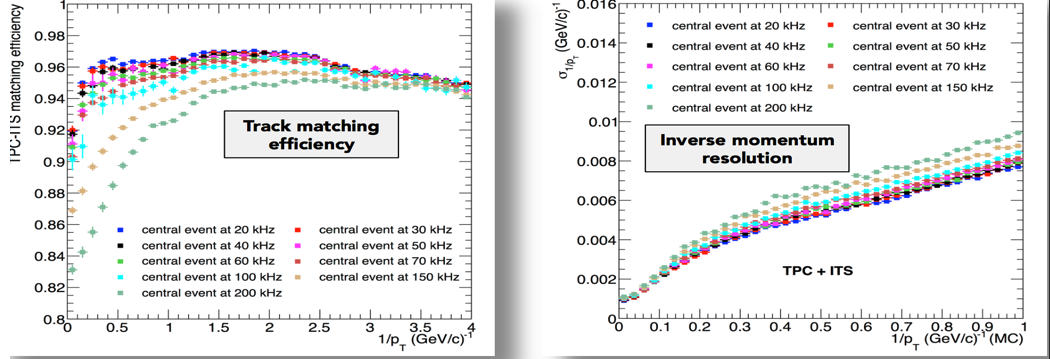
\includegraphics[width=\linewidth]{ResoSim}
\centering
\caption{ITS-TPC matching  \textit{(left)} and inverse momentum resolution \textit{(right)} for a 4-GEM stack simulated in Garfield++ \cite{Dick2017QM}. }
\label{fig:ResoSim}
\end{figure}

\noindent
Figure \ref{fig:ResoSim} shows simulations of the track matching efficiency from the ITS to the TPC and the inverse momentum resolution for a 4-GEM stack as a function of the collision rate.  The efficiency and resolution only start to diminish at an event rate above 100 kHz, which is double the expected rate after the LHC upgrade, and are well within the range of the current TPC operating at 3.5 kHz.
 
\begin{figure}[h]
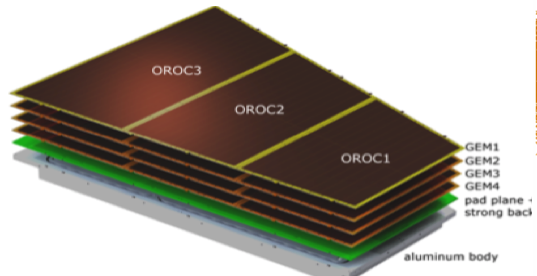
\includegraphics[width=10.0cm]{4GEMROC}
\centering
\caption{Final design of the upgraded readout chambers with a stack of 4 GEMS \cite{CERN-LHCC-2013-020}. }
\label{fig:4GEM}
\end{figure}

The optimal hole configuration was also explored with simulations.  Having a first and forth layer with a pitch of 140 $\mu m$ and the second and third layer with a pitch of 280 $\mu m$, allowed for the the ROCs to maintain minimal ion backflow while amplifying the signal from tracks.  Figure \ref{fig:4GEM} shows the design of the ROCs with a 4-GEM stack, the copper pad plane is glued to a reinforced fiberglass sheet , known as the strongback, to add material strength.

\subsubsection{2014 Test Beam}

The 2014 test beam served as my first task at CERN and introduced me to the TPC, GEMs, and ROCs.  I helped with setting up the prototypes on the beam line, recording data from the test beam, and monitoring the performance in real time.  To quantify the performances of the prototype it is useful to define the ionic backflow (IBF\%) as

\begin{equation}
IBF \% = \frac{ I_{cathode} }{ I_{anode} } = \frac{1 + \epsilon }{ G_{eff} }
\label{eq:IBF}
\end{equation}

\noindent
where $ I_{cathode} / I_{anode}$ is the ratio of the currents measured in the cathode and anode portion of a readout as seen in Figure \ref{fig:TPCreadout}.  The IBF\% can also be defined in terms of the number of backflowing ions ($\epsilon$) created at an effective gain ($G_{eff}$).  The effective gain is a measure of the amplification properties and in a gaseous detector is defined as

\begin{equation}
G_{eff}=\frac{I_{anode}}{\textit{e} \,  N_{ion} \ R}
\label{eq:gain}
\end{equation}
\noindent
where $\textit{e}$ is the fundamental electric charge of an electron, $N_{ion}$ is the numbered of captured ions, and R is the illumination rate from an active source.  The test involved using the beam from both the SPS and PS\footnote{See Section \ref{sec:LHCop}.} at the LHC cast onto an iron target.  This iron target created secondary showers and tracks were measured by the prototype for both energy resolution and PID performance.  The nominal TPC gas of $CO_{2}-N_{2}\,$(90-10) was used during the test beam.  

\begin{figure}[h]
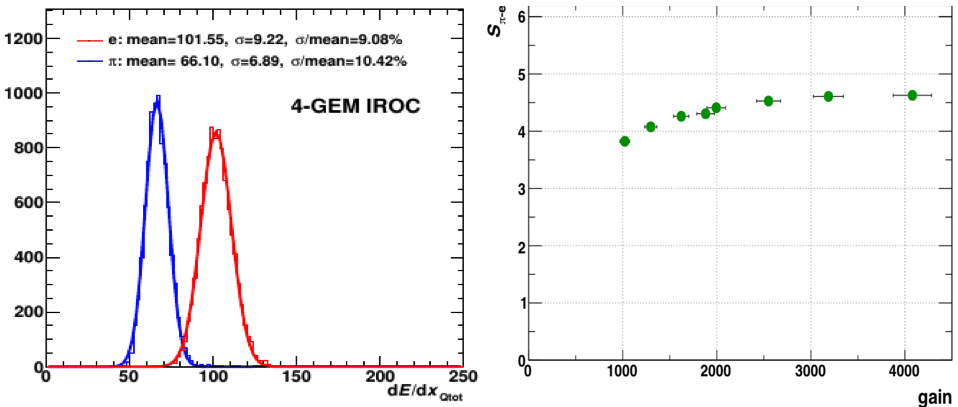
\includegraphics[width=10.0cm]{GemProtoPID}
\centering
\caption{dE/dx resolution of the 4-GEM IROC prototype\textit{(left)} and the separation power between electrons and pions as a function of gain \textit{(right)}\cite{CERN-LHCC-2015-002}.}\

\label{fig:GemProtoPID}
\end{figure}

Figure \ref{fig:GemProtoPID} shows the PID performance for separating electron and pion tracks created by the iron target, the separation power between the two Gaussian peaks trivially increases above a gain of 2000 and this was chosen as the target effective gain for the new ROCs.

% TALK ABOUT IROC DESIGN


\begin{figure}[h]
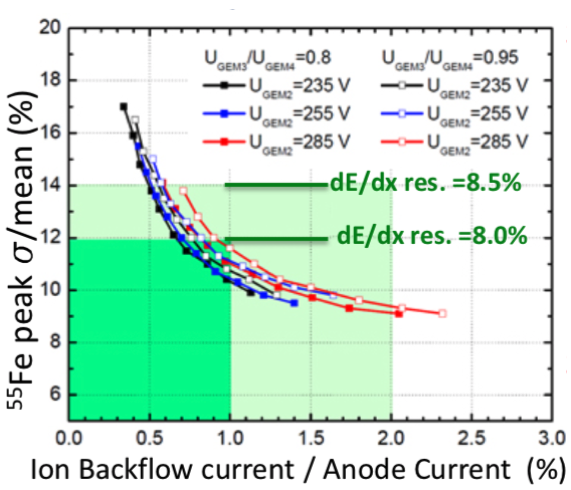
\includegraphics[width=6.0cm]{ProtoIBFEres}
\centering
\caption{Energy resolution of the iron peak as measured from the prototype IROC with varying GEM voltages as a function of IBF\%\cite{CERN-LHCC-2015-002}.}
\label{fig:ProtoIBFEres}
\end{figure}

\noindent
Figure \ref{fig:ProtoIBFEres} shows the energy resolution of the iron peak as a function of the relative voltages between GEM 2 ($U_{GEM2}$) and the ratio of voltages between GEM 3 ($U_{GEM3}$) and GEM 4 ($U_{GEM4}$) and shows that the IBF\% remains below 1\% at a energy resolution of $\approx 10\%$ which is consistent with the currant TPC performance.  The voltages were chosen such that GEM 1 and GEM2, which are closest to the drift volume, would focus mostly on capturing amplification ions while GEM 3 and GEM 4, which are closest to the copper pad readout, would primarily perform the amplification as shown in Figure \ref{fig:showersim}.

\begin{figure}[h]
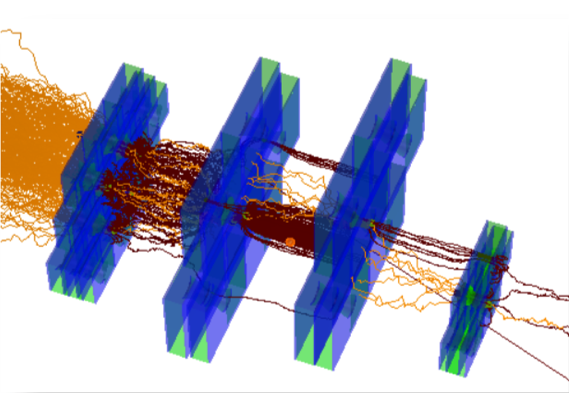
\includegraphics[width=8.0cm]{GEMShowerSim}
\centering
\caption{Simulation of the four GEM (blue) layers after test beam.  The configuration is such that the two GEMs closest to the drift volume, right side, absorb the amplification ions created by the two GEMs closest to the readout (right) \cite{CERN-LHCC-2015-002}.}
\label{fig:showersim}
\end{figure}



\subsection{Production of the Inner Readout Chambers in the U.S.}
Once a final design was settled on from the simulation and prototype portion of the G\&D we entered the production phase.  A minimum of 36 new ROCs would need to be built with the 4-GEM stack to replace the old ROCs in the TPC while 4 additional ROCs would be constructed as backups.  Due to the size and weight of the ROCs, production of the IROCs would take place in the United States and the OROC production mainly in Germany. 



\begin{figure}[h]
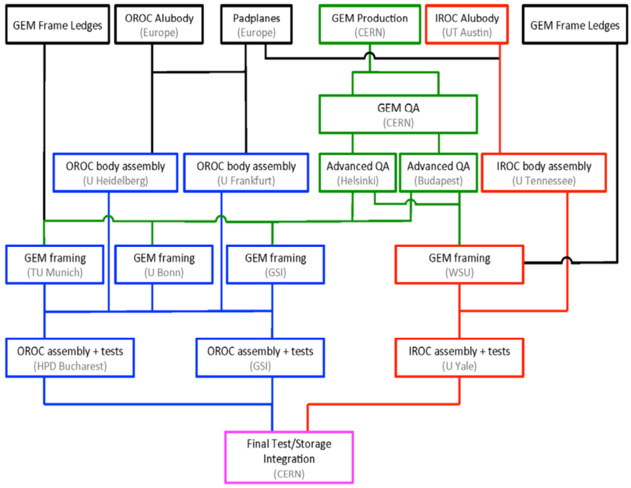
\includegraphics[width=10.0cm]{IROCproductionflow}
\centering
\caption{Production flow of the IROCs (red), OROCs (blue), and GEM foils (green)\cite{Dick2017QM}. }
\label{fig:IROCprod}
\end{figure}

\noindent
Figure \ref{fig:IROCprod} shows the production flow for the construction of the 4-GEM ROCs.  After GEMs are received from the manufacturer they go through a number of quality assurance tests before they are shipped to the institute responsible for framing and stretching them.  Wayne State University is responsible for the GEM stretching and mounting for the IROCs.   The aluminum bodies at the University of Texas Austin and shipped to Tennessee.  At Tennessee we glue the pad plane, aluminum body and strong back together before it is shipped to Yale where the chambers are fit with the GEMs from Wayne State.  The production steps for the OROC mirror those performed by the IROC except that it was performed by mainly German institutes.

\begin{figure}[h!]
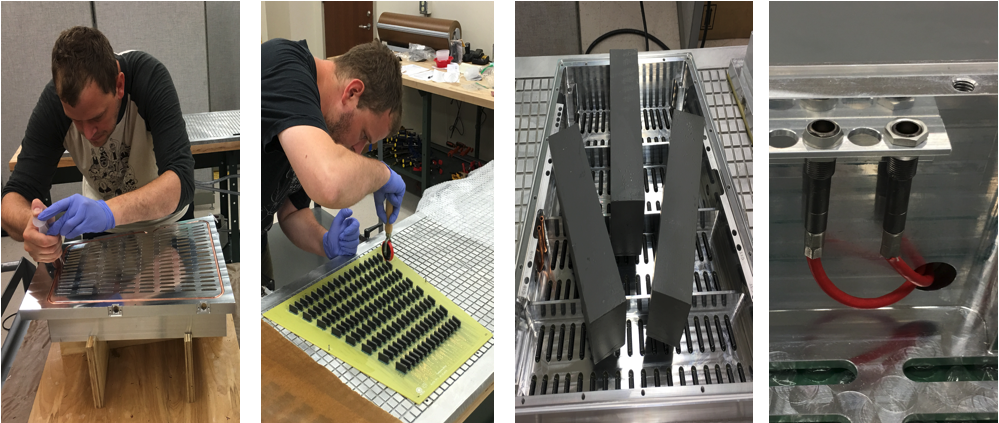
\includegraphics[width=\linewidth]{IROCAssemblyUTK}
\centering
\caption{The author assemblying an Inner Readout Chamber at the University of Tennessee \textit{(Courtesy of Andrew Castro)}. }
\label{fig:IROCassm}
\end{figure}

Figure \ref{fig:IROCassm} shows the procedure followed at Tennessee in order to build an IROC.  Furthest on the left is a picture of gluing a copper pipe into the aluminum body.  This copper pipe is flushed with a colant that maintains the temperature of the Front End Electronics (FEE).  The next two photos of Figure \ref{fig:IROCassm} show the pad plane mounted on a vacuum table while glue is applied to it and the aluminum body.  Once the two are aligned the glued IROC lead bricks are placed on the ROC and the epoxy is allowed to cure for 24 hours.  The right most picture shows the final step of mounting and gluing the HV feedthroughs for the GEM foils.  Before a completed IROC leaves Tennessee we performed a gas tightness test that will be discussed more in the next section.
Full production of the IROCs ended in November of 2018 with a total of 47 chambers being built at Tennessee.  A surplus of chambers was built due to excess materials we had.


\subsection{GEM and Chamber Quality Assurance}
Due to the large amount of work outsourced to numerous universities, international labs, and private contracts for the TPC upgrade, a stringent set of quality assurance (QA)\cite{Brucken:2018rej}\cite{Brucken:2017qjy} protocols were implemented to monitor any damaged sustained during transport and to quickly identify any flaws in the production procedures.  The QA can be broken into two major categories: QA performed on the GEM foils as received from the manufacturer and QA performed on complete/semi-complete chambers as they were going through the different production steps.  I will discuss only the QA tasks that I was directly involved with.

\subsubsection{GEM QA}

In order to evaluate the performance of a GEM foil, a spark test was performed on every foil.  Sparks are caused by the discharge of the foil and may be due to the presence of dust on a foil, imperfections in the hole geometry, or a short between the two copper layers of the GEM.  The final design of the GEM foils had each foil segmented into twelve sectors with a 10$\: M \Omega$ bias resistor across every segment.  Any sparks that occur on the GEM will only discharge a given segment and not the entire foil.  Because of the delicate nature of the GEM foil, sparks have the potential to permanently damage a foil or seriously affect the performance of a ROC.  Thus GEMs with a high spark rate should be excluded as soon as possible in the production flow.

\begin{figure}[h]
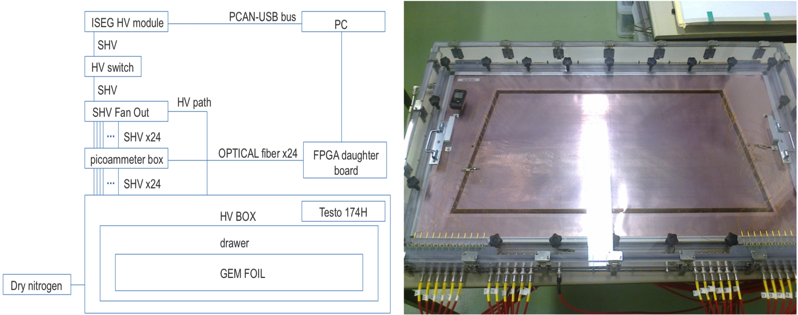
\includegraphics[width=\linewidth]{PicoSetup}
\centering
\caption{Schematic for the setup of the GEM foil spark test (\textit{left})\cite{Brucken:2018rej} and the GEM mounted in the HV gas box (\textit{right}). }
\label{fig:PicoSetup}
\end{figure}

\noindent
The GEM foil spark test involves mounting each foil in a High Voltage (HV) box, which is flushed with $N_{2}$ until it reaches a relative humidity of $\approx 10\%$.  Once this humidity is reached 500 V is placed across each segment of the GEM and and monitored with a LabView interface.  A spark is defined as the LabView recording a current above 10 nA across the bias resistor through any GEM segment and read by a multi-channel picoammeter.  The criteria for a GEM to fail this QA was to have more than five sparks over a 20 minute recording window.

\subsubsection{Chamber QA}

Most of the QA I helped with was on ROC chambers as they went through the production steps.  Before completed IROC chambers were sent to Yale, I performed a gas leak test.  The leak test consisted of mounting an individual chamber into an aluminum test vessel and flushing the inside of the vessel with $N_{2}$ gas.  By using a flowmeter to measure the rate that $N_{2}$ gas enters the test vessel and an oxygen sensor to measure the amount of oxygen present at the output of the test vessel we can infer the leak rate of each IROC chamber.  Figure \ref{fig:LeakTest} shows a schematic of the setup (left) and what the typical output from the LabView interface (right).  By flowing at two different rates and measuring the oxygen content at each rate we could confirm the leak rate.

\begin{figure}[h]
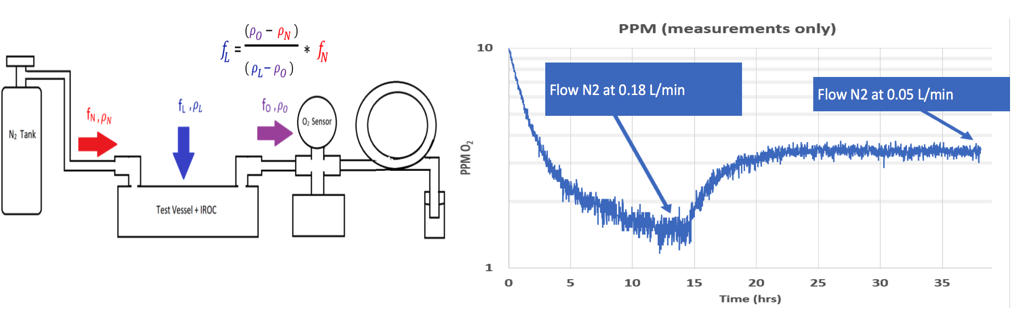
\includegraphics[width=\linewidth]{LeakSetupUTK}
\centering
\caption{Schematic of the gas tightness testing setup at the University of Tennessee \textit{(Courtesy of Joseph Rasson)}. }
\label{fig:LeakTest}
\end{figure}

\noindent 
The leak rate of a chamber, $\mathit{f_{L}}$,  can be quantified as
\begin{equation}
\mathit{f_{L}} =\Bigg(  \frac{\rho_{0} -\rho_{N}}{\rho_{L} -\rho_{0}} \Bigg) \,  \mathit{f_{N}}
\label{eq:leakrate}
\end{equation}

\noindent
where $\mathit{f_{N}}$ is the flow rate of $N_{2}$ gas into the test vessel, $\rho_{L}$ is the concentration of $O_{2}$ in the laboratory, $\rho_{N}$ is the $O_{2}$ impurity present in the $N_{2}$ bottle, and $\rho_{0}$ is the $O_{2}$ reading from the LabView interface.  

\begin{figure}[h]
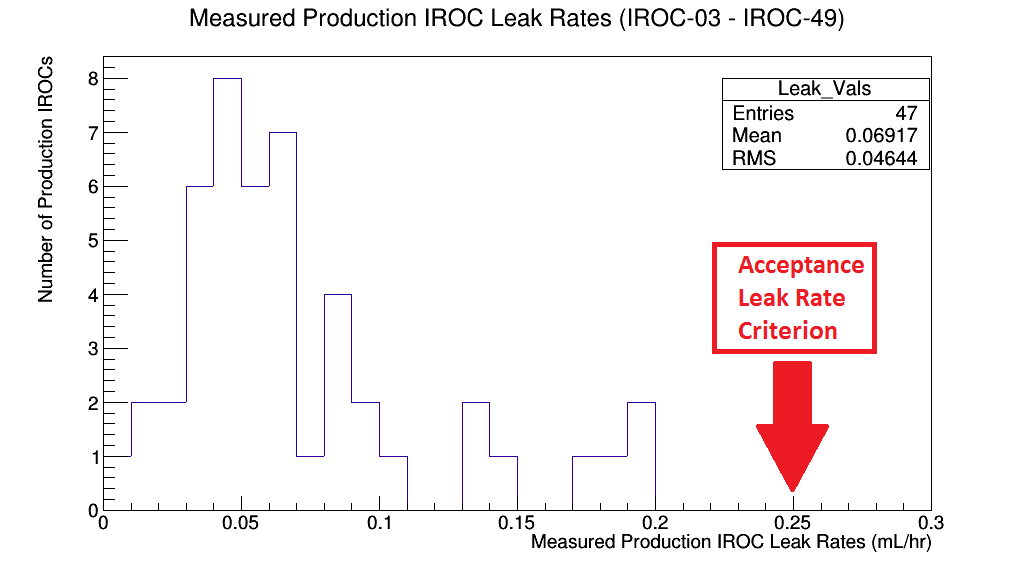
\includegraphics[width=8.0cm]{AcceptanceCriteria}
\centering
\caption{Leak rate of the 47 chambers built at Tennessee with the maximum failure rate at 0.25 ml/hr shown \textit{(Courtesy of Charles Hughes)}. }
\label{fig:IROCprod}
\end{figure}


A maximum leak rate of 0.25 mL/hour was placed as the rejection criteria for a given chamber.  If a chamber had a leak rate above this the $N_{2}$ gas could get swapped out with a helium gas tank and we could use a helium sniffer to identify the areas on the IROC causing the leak and patch the area with epoxy.  Figure \ref{fig:IROCprod} shows the leak rate for all IROCs produced at Tennessee, due to none of the chambers surpassing the leak threshold the helium sniffer was not used in the production of the IROCs. 

Once an IROC chamber was fitted with the 4 GEM foils at Yale and sent to CERN a spark test was performed over the entire chamber.  The test involved placing each chamber next to the LHC beam line, flushing with the nominal TPC gas, and placing the nominal voltage across each GEM and monitoring the spark rate once a beam was present in the LHC.   Figure \ref{fig:LHCspark} shows myself installing the completed IROC chambers next to the LHC beam line in front of ALICE and the output from the spark monitor.  The voltage across each chamber could be varied in real time in order to minimize sparking while maintaining the IROC performance, thus reducing the rate of degradation on a per chamber basis once installed in the TPC.




\begin{figure}[h]
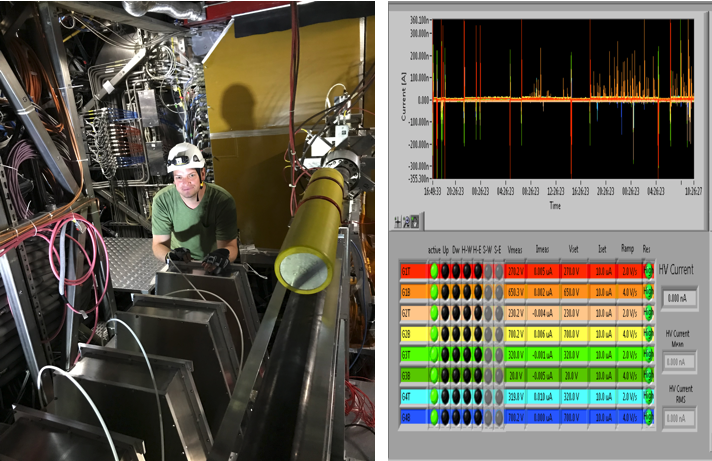
\includegraphics[width=14.0cm]{LHCSparkTest}
\centering
\caption{The author testing spark testing chambers next to the LHC beam line \textit{(left)} and real time output from the spark test during a live beam (\textit{right}). }
\label{fig:LHCspark}
\end{figure}




%\subsection{Upgrade of the TPC Front-End Cards}
%The TPC is expected to see a factor of x100 increase in MinBias data and a factor x10 increase in high-$p_{t}$ data after the Hi-Lumi upgrade.  This necessitates an upgrade of the front-end electronics to continuously sample events and to transfer the signal from events of interest to a disk farm.

\subsection{Outlook}

As of November 2018, the 47 IROCs assembled at Tennessee have been received at CERN.  None of the built chambers have surpassed the gas leak test performed at CERN and so far only 4 chambers exhibit sparking rates above the threshold.  By May of 2019, the LHC beamline around ALICE will be decommissioned and the TPC will be moved to a surface level clean room for the installation of the chambers.  The installation of the new FEE electronics and the ROC chambers should take place throughout the summer of 2019.  Afterwards there will be a 10 month commissioning with the TPC, during which the performance of the upgraded TPC will be evaluated with cosmic rays.  By the end of 2020, the TPC should be back in the ALICE cavern and the beam line will have been re-installed.  The Hi-Lumi run of the LHC is expected to start in March of 2021.






    \chapter{Jet Results and Discussion} \label{ch:analysis}

Beginning in March of 2012, the LHC began seven months of pp collisions at $\sqrt{s} = \,$ 8 TeV.  The jet cross sections and ratios of the cross sections for jets of different radii offers a unique perspective on the pQCD effects of hadronization at this new energy frontier.  Due to the expectation that no QGP is formed in a pp collision these measurements serve as a baseline for separating phenomena associated with the QGP in heavy-ion collisions.  In order to measure the jet cross section the following formula is used,

\begin{equation}
	\frac{d^{2} \sigma^{jet}}{d\eta \, dp_{T}} = \frac{A_{trigger}}{\epsilon_{trigger}(p_{T})} \times C_{MC} \times \frac{1}{A(p_{T}) } \times \frac{1}{\mathscr{L}_{int}} \times \frac{dN^{jet}}{dp_{T} \, d\eta}
\label{eq:xsecdef}
\end{equation}

\noindent
where,

\begin{itemize}
  \item $A_{trigger}$ is the acceptance for EMCal triggered events and $\epsilon_{trigger}(p_{T})$ is the EMCal trigger efficiency.  These factors correct for imperfections in the electronics of the EMCal and the overall factors are equal to one in minimum bias events.
  \item $C_{MC}$ is a correction factor due to detector effects and it allows for comparisons between the ALICE experiment to other experiments or theoretical calculations.  Unfolding is used to determine this factor.
  \item $\mathscr{L}_{int}$ is the integrated luminosity during the period when the data was recorded.
  \item $A(p_{T})$ is the geometrical detector acceptance.
  \item $\frac{dN^{jet}}{dp_{T} \, d\eta}$ is the inclusive jet momentum spectra.
  
\end{itemize}

\noindent
Furthermore, it is useful to define the ratio of cross sections,

\begin{equation}
\mathscr{R}(p_{T};R_{1},R_{2}) = \frac{d^{2}\sigma(p_{T};R_{1})/d\eta \, dp_{T}}{d^{2}\sigma(p_{T};R_{2})/d\eta \, dp_{T}}
\label{eq:xsecratio}
\end{equation}

\noindent
where $\sigma(p_{T};R_{1})$ refers to the doubly differential cross section (Equation \ref{eq:xsecdef}) of a jet with radius $R_{1}$.  The ratio is carried out on a bin--by--bin basis per each $p_{T}$ bin.  

\section{Raw Jet Spectra}

This thesis measured inclusive jet results for radii between 0.1 and 0.5.  Furthermore, jet results for radii R = 0.2 to R = 0.4 will be presented in the body of this chapter while results from the other jet radii are still being investigated.  Figures \ref{fig:rawjetR02} \ref{fig:rawjetR03} \ref{fig:rawjetR04} show the raw (uncorrected) $p_{T}$ spectra for inclusive jets from both MB and EMCal triggered data.  It is also evident from Figures that the EMCal triggered data extends the $p_{T}$ reach of the spectra.

\begin{figure}[h]
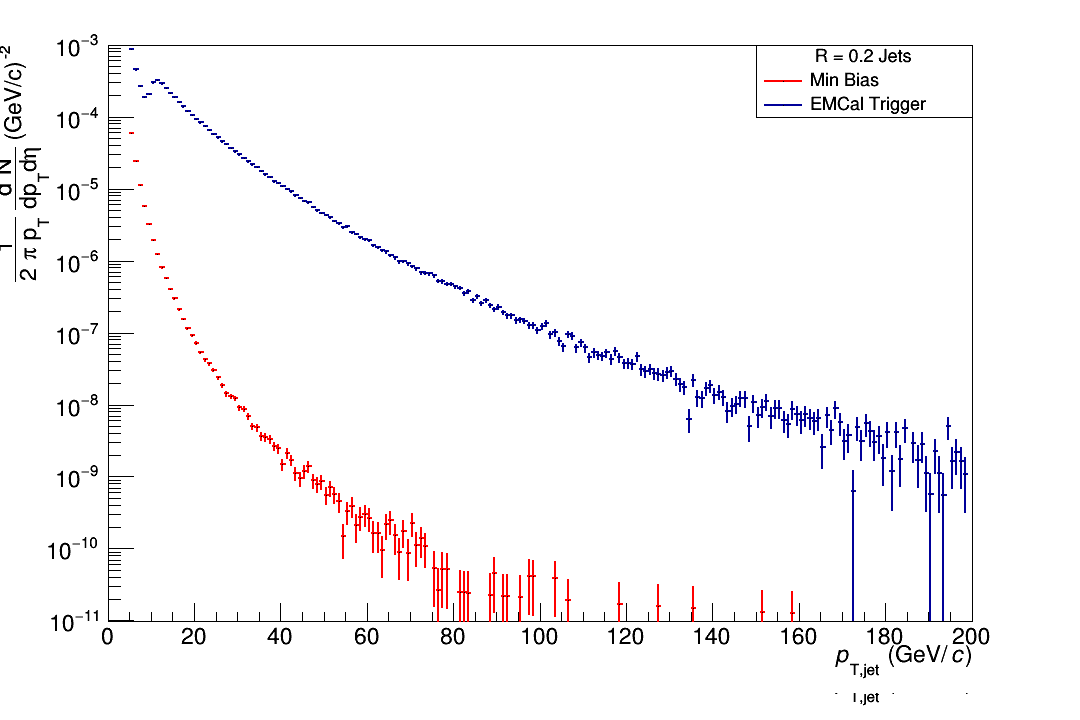
\includegraphics[width=10cm]{RawR02JetSpectra}
\centering
\caption{Raw inclusive R = 0.2 jet spectra from the 8 TeV Min Bias and EMCal triggered data}
\label{fig:rawjetR02}
\end{figure}
\begin{figure}[h]
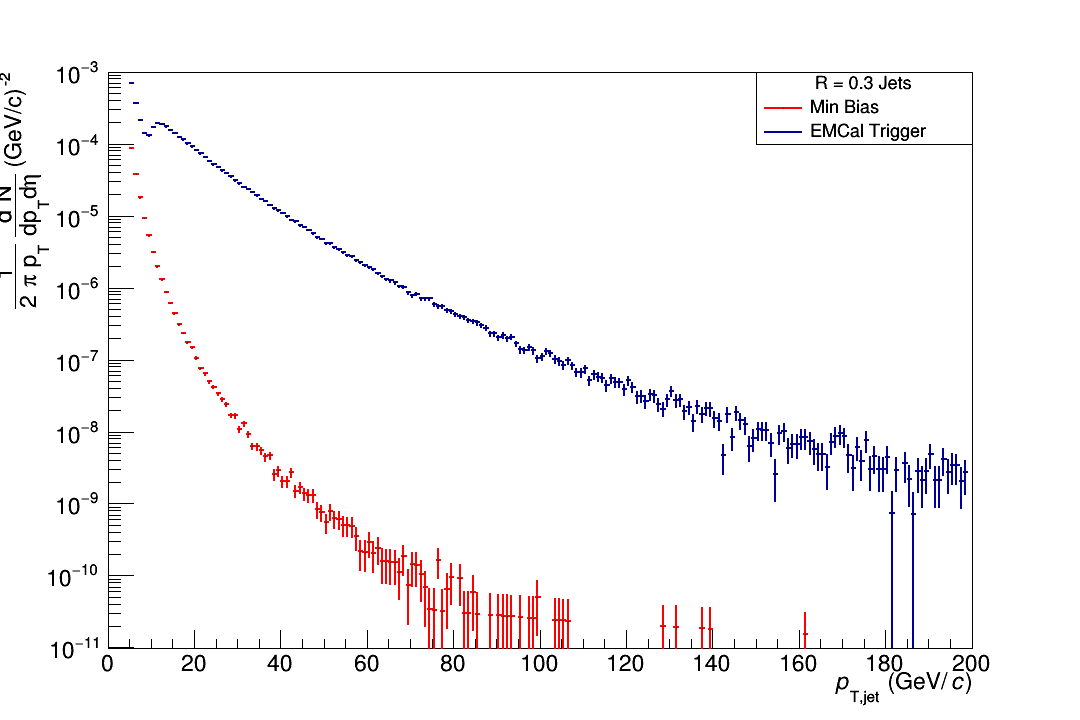
\includegraphics[width=10cm]{RawR03JetSpectra}
\centering
\caption{Raw inclusive R = 0.3 jet spectra from the 8 TeV Min Bias and EMCal triggered data}
\label{fig:rawjetR03}
\end{figure}
\begin{figure}[h]
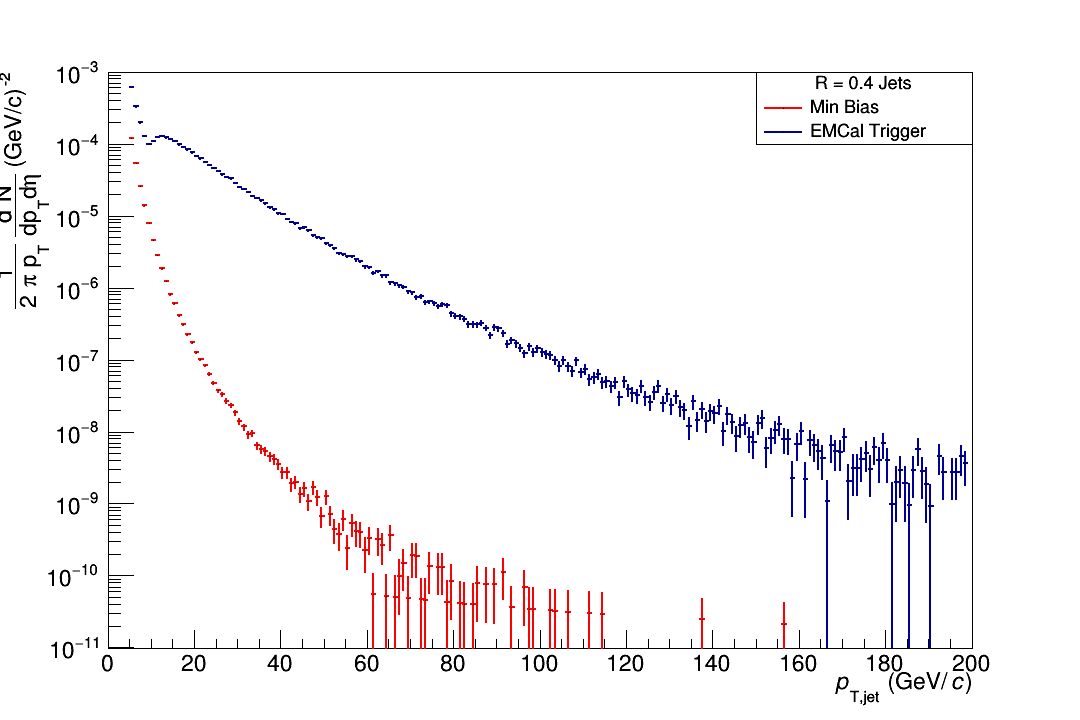
\includegraphics[width=10cm]{RawR04JetSpectra}
\centering
\caption{Raw inclusive R = 0.4 jet spectra from the 8 TeV Min Bias and EMCal triggered data}
\label{fig:rawjetR04}
\end{figure}

\noindent
The next sections of this chapter will discuss the QA implemented to the data, trigger scaling, unfolding, and other corrections 

\section{8 TeV Data Quality}
ALICE is a state-of-the-art experiment with excellent tracking and particle identification capabilities as discussed in Chapter \ref{ch:alice}.  However, just like any real world experiment, it contains a number of inefficiencies and imperfections.  This means that the data collected during the 8 TeV pp collision must be examined and any inaccuracies in the data must be removed before hard physics conclusions may be reached.  Data may be compromised at both the event-level, the experiment erroneously recorded something as an event, or at the constituent-level, one of the subdetectors mismeasured a feature of a particle, and these outliers must be accounted for and removed 

\section{Event Selection}


\begin{figure}[h]
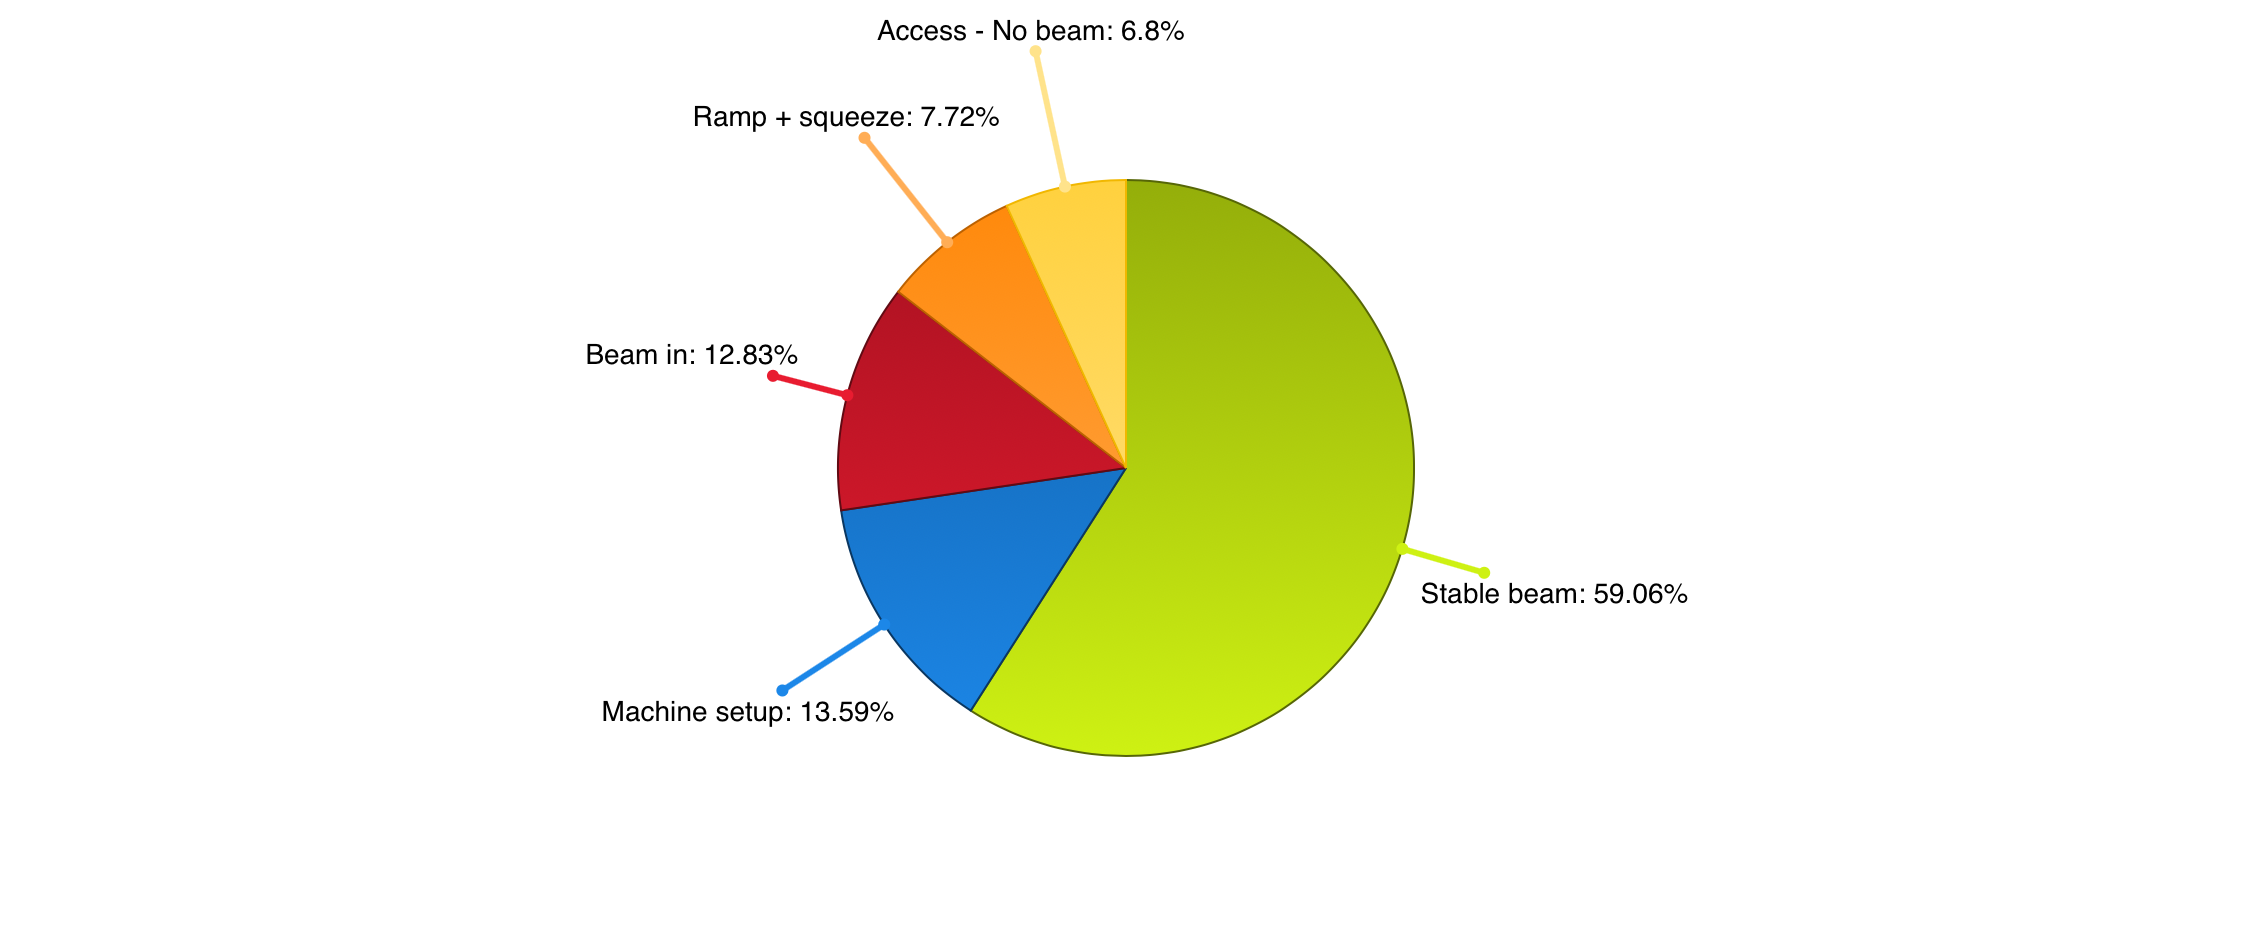
\includegraphics[width=17cm]{8TeVRunefficency}
\centering
\caption{LHC state during the 8 TeV run. }
\label{fig:RunEff}
\end{figure}

During the 8 TeV data collection period approximately 180 million minimum bias events were recorded, as summarized in table \ref{tab:RunSummary}.  These events are separated into periods, which dictate the particular beam and detector configurations during the data taking.The 8 TeV data is broken into 7 periods with approximately 181 million minimum bias events recorded.  This minimum bias sample corresponds to an integrated luminosity, $\mathscr{L}_{int}$, of $8.95 \, pb^{-1}$ during this time period\cite{ALICE-PUBLIC-2017-002}.

\begin{table}[hb]
\label{tab:RunSummary}
\begin{center}
\begin{tabular}[b]{|c|c|c|}
	\hline
	Period & \# of runs & \# of Min Bias events \\ \hline
	LHC12c & 89 & $\sim \,$24 M \\ \hline
	LHC12d & 140 & $\sim \,$62 M \\ \hline
	LHC12e & 5 & $\sim \,$2 M \\ \hline
	LHC12f & 56 & $\sim \,$15 M \\ \hline
	LHC12g & 8 & $\sim \,$0.4 M \\ \hline
	LHC12h & 159 & $\sim \,$75 M \\ \hline
	LHC12i & 40 & $\sim \,$3 M \\ \hline
	Total & 497 & $\sim \,$181 M \\ \hline

\end{tabular}
\end{center}
\caption{2012 8 TeV data taking period.}
\end{table}

Approximately, 15\% of the data sampled is unusable due to malfunctions in TPC chambers, EMCal super modules, the electronics for the EMCal or TPC, and   

For an event to be selected into a physics analysis it must pass a number of quality control tests.  For example, the LHC must have be in a state of stable beams, cosmic rays must be excluded by only accepting tracks that originate from a vertex inside the detector, and the relevant detectors for a given analysis must be functioning as intended.  Event selection and QA is implemented via a centralized class, AliEventCuts, within the AliRoot framework.  This class contains a number of corrections including:

\begin{itemize}
  \item The event has a primary vertex reconstructed.
  \item The primary vertex occurs within a 10 cm window of the primary interaction point.
  \item The vertex resolution must be below 0.25 cm.
  \item The event passes basic pile-up checks based on the V0 and T0 signals.
\end{itemize}

\noindent
A summary of the rejection reasons at the event level is summarized in Figure \ref{fig:eventqa}.

\begin{figure}[h]
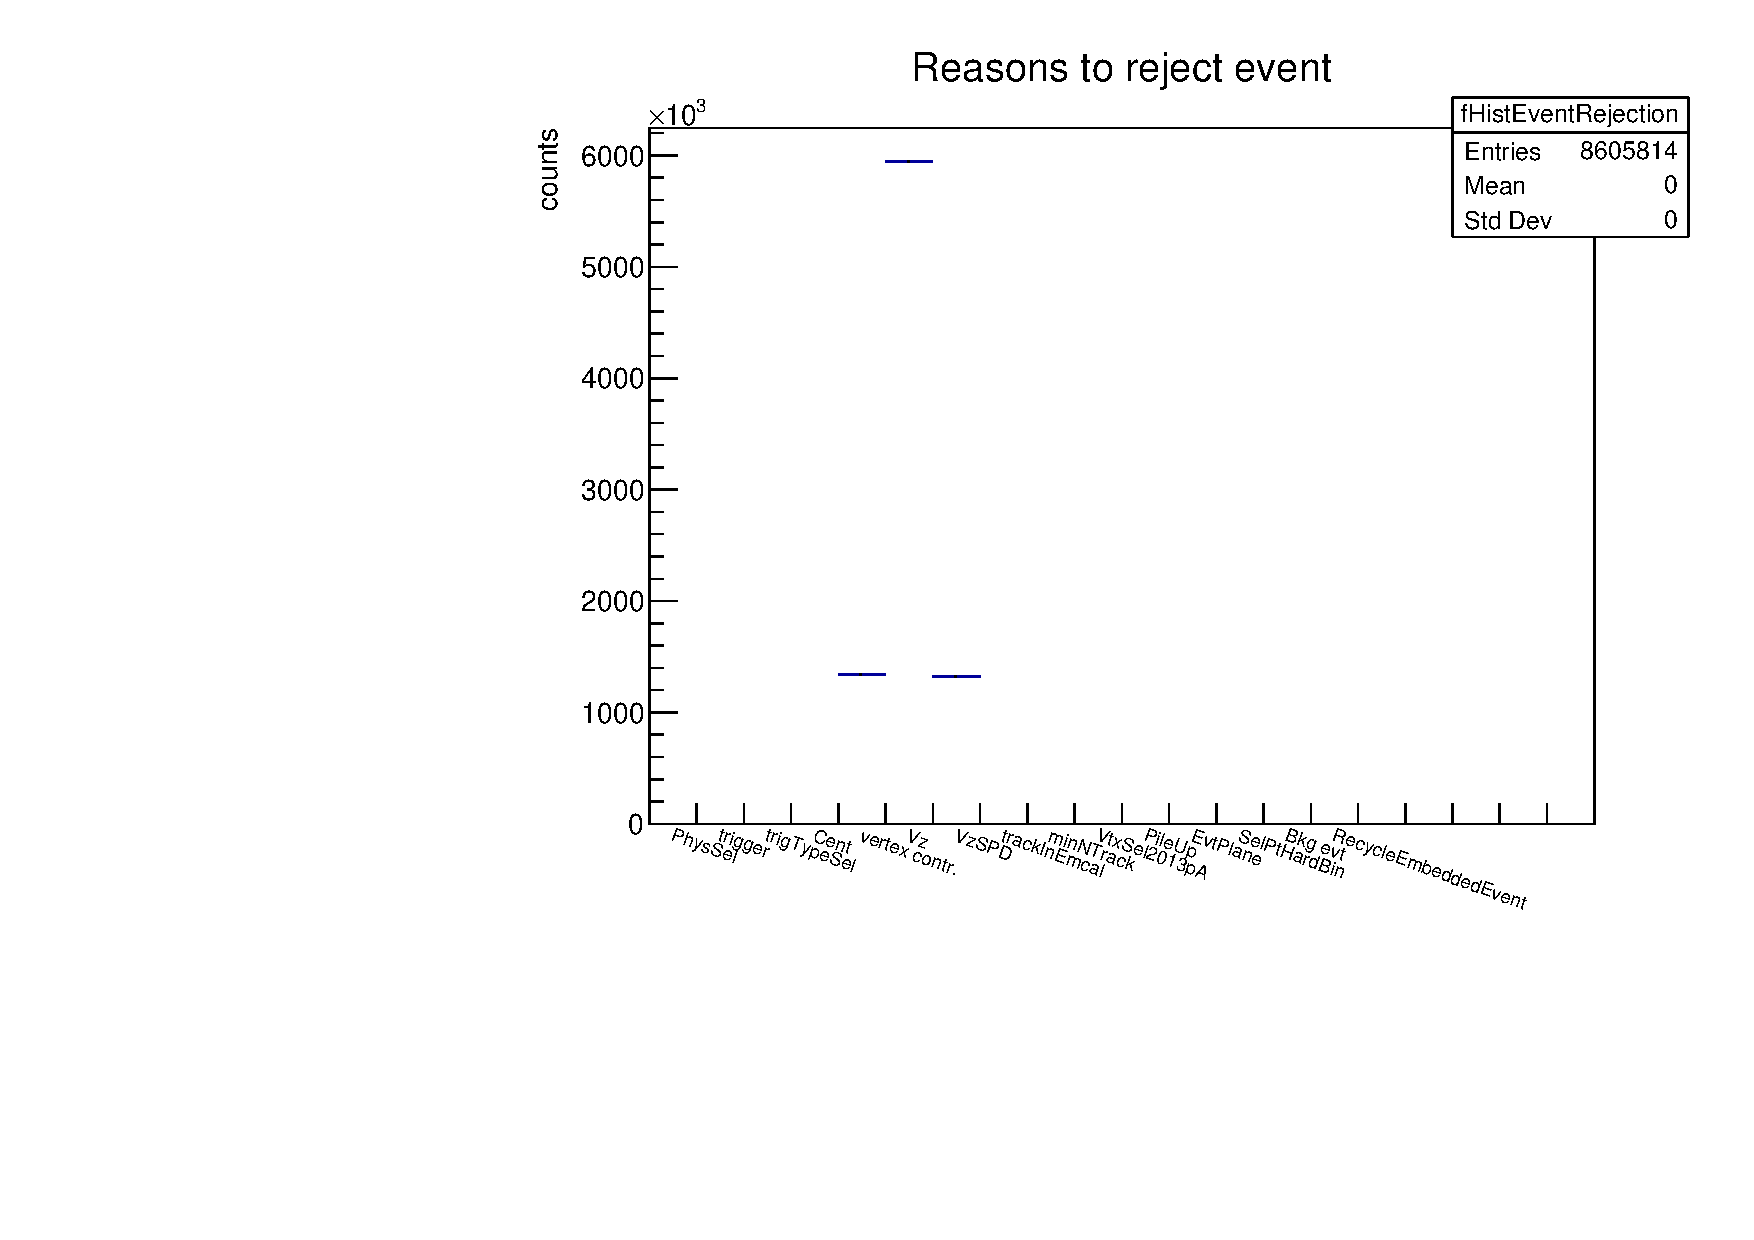
\includegraphics[width=10cm]{RejectionReasons}
\centering
\caption{Min Bias event rejection summary.}
\label{fig:eventqa}
\end{figure}

\begin{figure}[h]
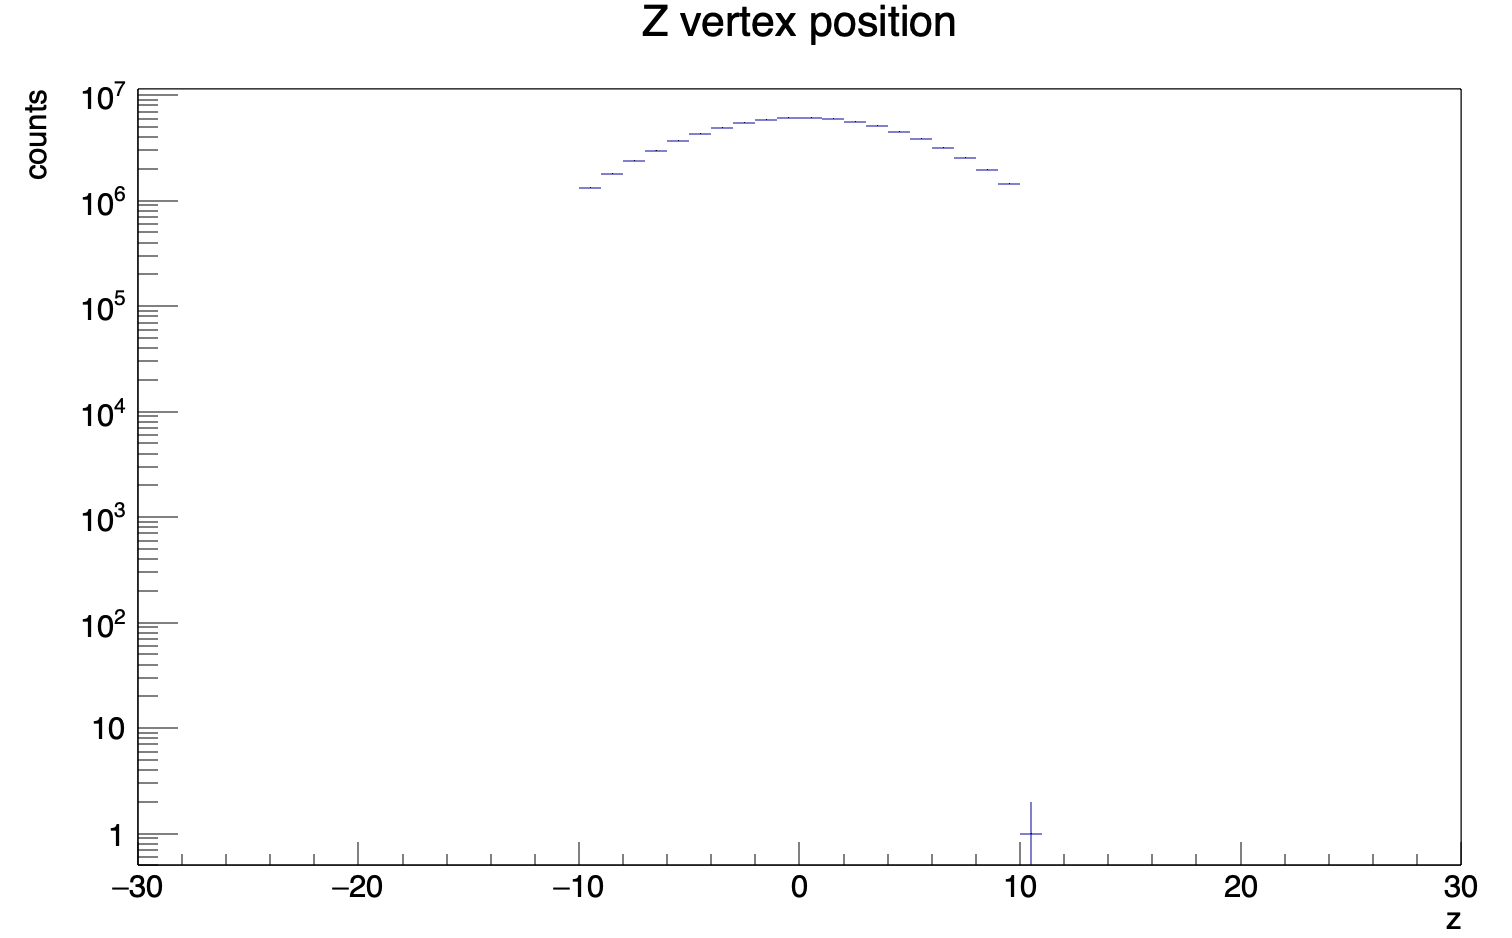
\includegraphics[width=10cm]{zvertex}
\centering
\caption{Vertex displacement from primary interaction point for accepted Min Bias events.}
\label{fig:vertrec}
\end{figure}

\noindent 
Figure \ref{fig:vertrec} shows the reconstructed vertex for the accepted Min Bias events.  We see that the vertex distribution peaks at the primary interaction point as expected.  It should also be noted that a similar set of event QA was implemented to the EMCal triggered data \textit{(not shown)} and that the results were consistant with the Min Bias data.

\subsection{EMCal Cluster Selection}
Corrections are performed on EMCal cells including; removing hot and dead towers (bad channels) based on the average occupancy and energy of the towers, timing calibrations in order to remove slow particles such as $K_{0}^{L}$ and \textit{n}, and a energy calibration is implemented based on the $\pi^{0}$ mass.  After these corrections are applied to the towers are grouped together into clusters using the v2 algorithm.  The v2 algorithm has a minimum tower seed, $E_{seed} = \,$ 300 MeV, after which all adjacent towers with a minnimum energy, $E_{cell} \geq \,$ 100 MeV, are iteratively added until a local minimum is reached.  The cluster energy is the sum of the seed and grouped neighbor tower energies.   

\begin{figure}[h]
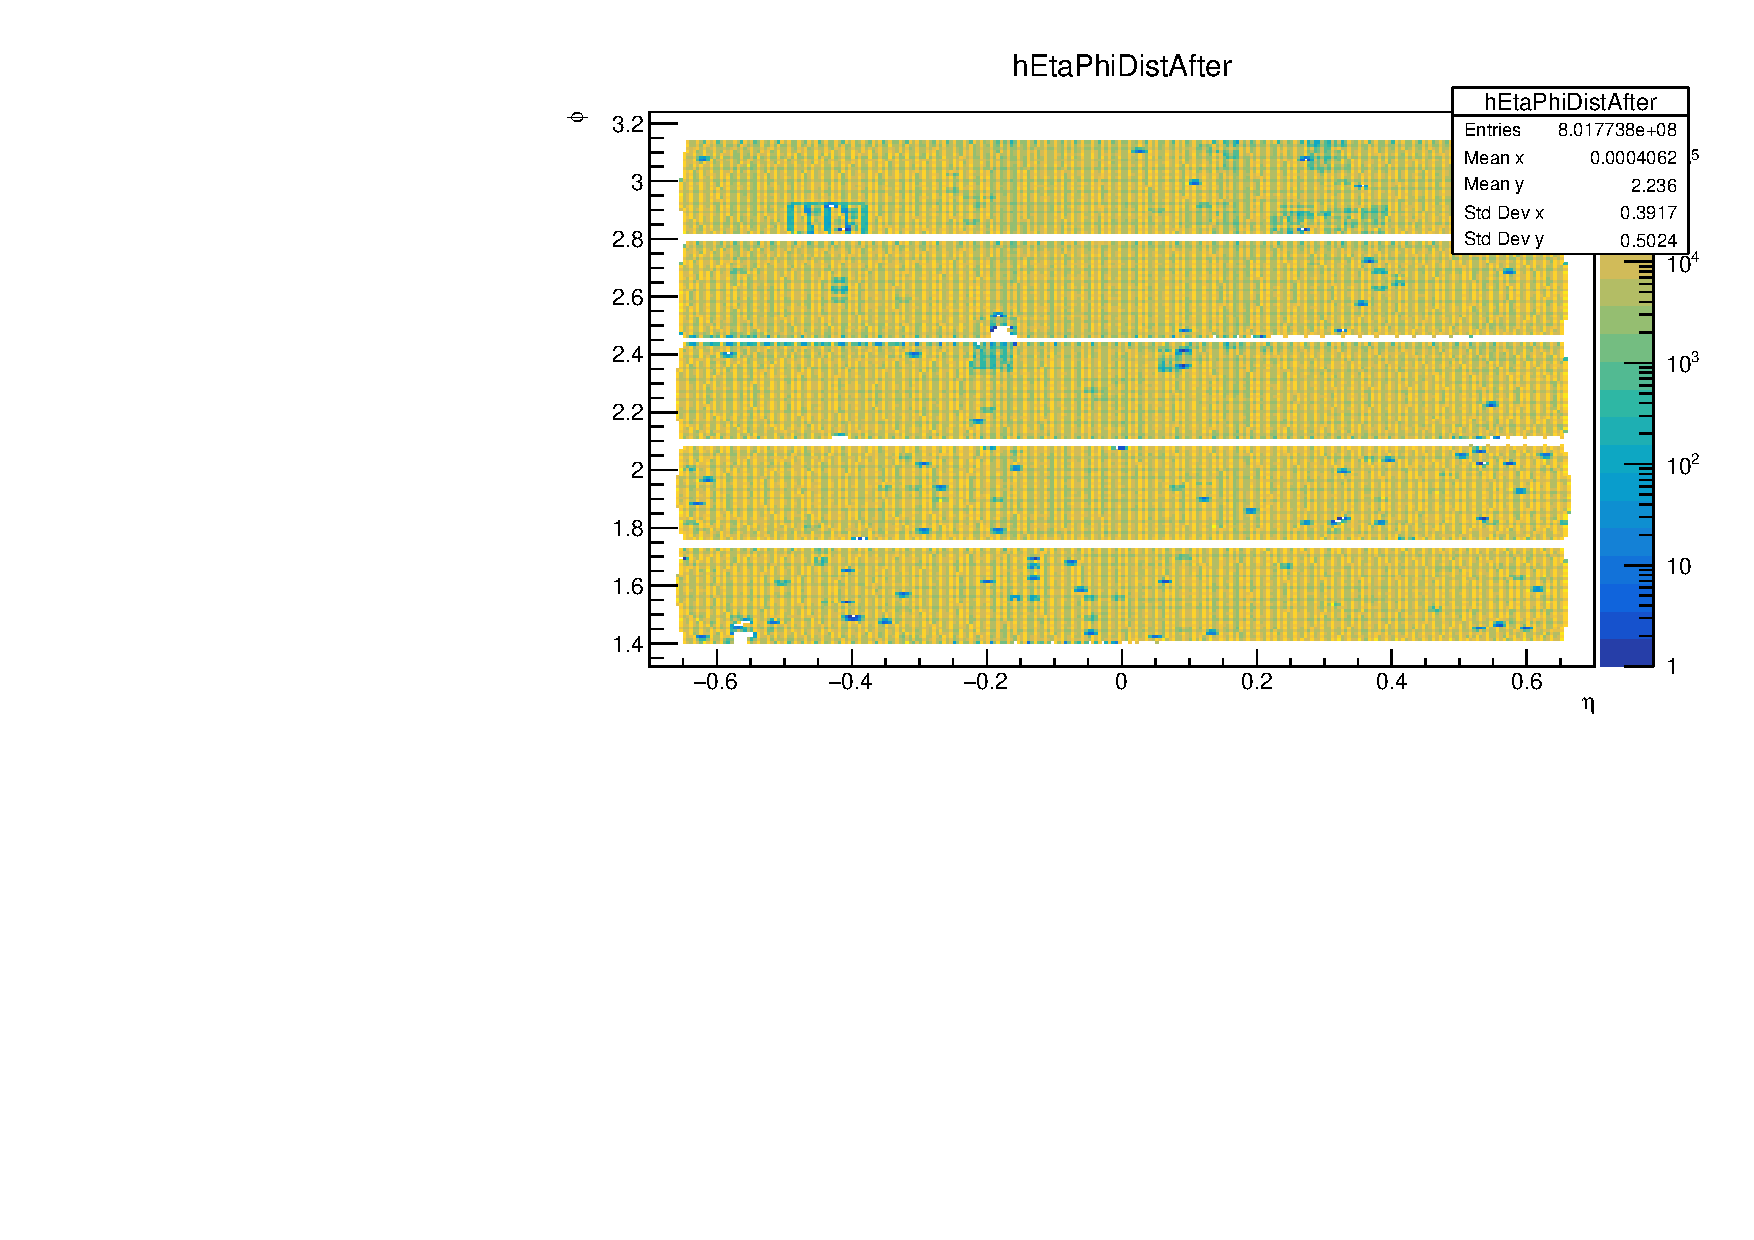
\includegraphics[width=14cm]{BadChannelMap}
\centering
\caption{EMCal cell occupancy after bad channels removed.}
\label{fig:badchannel}
\end{figure}

\subsection{TPC Track Selection}
\subsection{Raw Jet Momentum Spectra in pp Collisions}

\section{EMCal Triggered Data}

In addition with the minimum bias data collected, the EMCal was used during the 8 TeV run in order to provided an enhanced data set that is preferential to hard processes.   The Level-1 trigger\cite{Bourrion:2010js} in the EMCal has a associated trigger, $\epsilon$, of 

\begin{equation}
	\epsilon = \frac{N^{Triggered}_{events}}{N^{MinBias}_{events}} \times \frac{d^{2} N_{Triggered}^{jet}}{d\eta \, dp_{T}} \Bigg/  \frac{d^{2} N_{MinBias}^{jet}}{d\eta \, dp_{T}} 
\label{eq:xsecdef}
\end{equation}

\subsection{Acceptance Correction}
Jet spectra, cross sections, and ratios of cross sections are reported over the full azimuth angle and psuedorapidity acceptance.  However, due to jets being constrained to the EMCal, a geometric factor is used to correct for the limited acceptance of the detector.  This thesis uses a maximum jet radius of 0.5 to help study the effects of wide angle radiation on jet fragmentation.  Heavy-ion use smaller jet radii, typically of 0.2, to help negate the high multiplicity background.  Due to these geometric corrections the centroid of a jet is constrained to,

\begin{equation}
|\eta_{jet}| \leq 0.7 - R, \; 1.4 + R \leq \phi_{jet} \leq 3.14 -R.
\label{eq:jetconstration}
\end{equation}

\begin{equation}
A(p_{T}) = \frac{(1.4 - 2R) \times (1.745 - 2R)}{2 \pi}.
\label{eq:acceptance}
\end{equation}

For jets between R = 0.1 through R = 0.5 the following jet acceptance corrections are used.

\begin{table}[hb]
\label{tab:AcceptanceFactor}
\begin{center}
\begin{tabular}[b]{|c|c|c|}
	\hline
	Jet R & $A(p_{T})$ \\ \hline
	0.1 & 0.296 \\ \hline
	0.2 & 0.214\\ \hline
	0.3 & 0.146\\ \hline
	0.4 & 0.091\\ \hline
	0.5 & 0.048\\ \hline
\end{tabular}
\end{center}
\caption{EMCal jet acceptance for radii 0.1 - 0.5.}
\end{table}








\section{Unfolding}

The reconstructed jet $p_{T}$ has a number of detector effects `folded' into the measurement.  These effects included such things as:

\begin{itemize}
\item Tracking inefficiencies from the TPC and ITS.
\item Missing jet energy components from long-lived particles, such as the $K^{0}_{L}$ and neutron, that are cut by the EMCal timing requirement.
\item TPC track $p_{T}$ and EMCal cluster energy resolutions.
\item Hadronic corrections to the EMCal cluster spectrum.
\item Material loss in the detectors.
\end{itemize}

\noindent
Unfolding is the method by which these detector effects are removed from the raw inclusive jet spectra and a `true' jet spectra may be obtained and compared with theoretical calculations or other experimental results.  In order to unfold a jet spectra it is necessary to generate a response matrix that simulates the described effects above, after the response matrix is generated a number of statistical approaches including, Bayesian, Singular Value Decomposition (SVD), or Bin-by-Bin, may be applied to unfold the raw jet spectra.  In order to generate the response matrix we embed a Pythia generated event into a GEANT3 simulation of the ALICE detector.  Due to the fact that the performance and efficiency of the ALICE detector may change between the data taking periods each simulation is `anchored' to a given LHC, these anchors contain all the hot and dead sectors for the subdetectors, along with their calibrated performance during that specified data taking.  Two Monte Carlo data sets were produced with the MB trigger for the full 8 TeV run, the first was a Pythia generator using the Monesh-2013 tune and the second was a MB tune of the PHOjet Monte Carlo package.  Both data sets were explored for this thesis and it was decided that the final corrected spectra would be obtained via unfolding with the Pythia MC data set.  The magnitude of any one of the effects unfolding is supposed to account for is not expected to be very large, but combined may be significant, thus unfolding is an important step in this analysis.

\subsection{Response Matrix}
Given a truth-level particle jet $p_{T}$ we wish to reconstruct that jet's $p_{T}$ at the detector-level.  The particle-level pythia jets are constructed from the primary particles generated via Pythia while excluding any daughter decay particles in order to avoid double counting.  In addition the tracking efficiency in Pythia is known to deviate from nature.  This is due to Pythia under predicting the production of strange quarks.  
Constructing the response matrix in this case is calculated on a jet-by-jet basis.  The particle-level jet centroid ($\phi_{part}$,$\eta_{part}$)is matched to the detector-level jet via a constrain on the displaced distance between the two jet centroids in ($\phi$,$\eta$).  This distance was constrained to: $\Delta  R = \sqrt{(\phi_{part} - \phi_{det})^{2} + (\eta_{part} - \eta_{det})^{2}} \leq 0.25 \; $.  Once a jet is matched at the detector level to a jet generated from the particle level the response matrix is incremented by jet $p_{T}$ at both the detector and Monte Carlo levels.  The response matrix is generated with a fine binning with a width of 1 GeV per bin. 

\begin{figure*}[t!]
$\begin{array}{rl}
    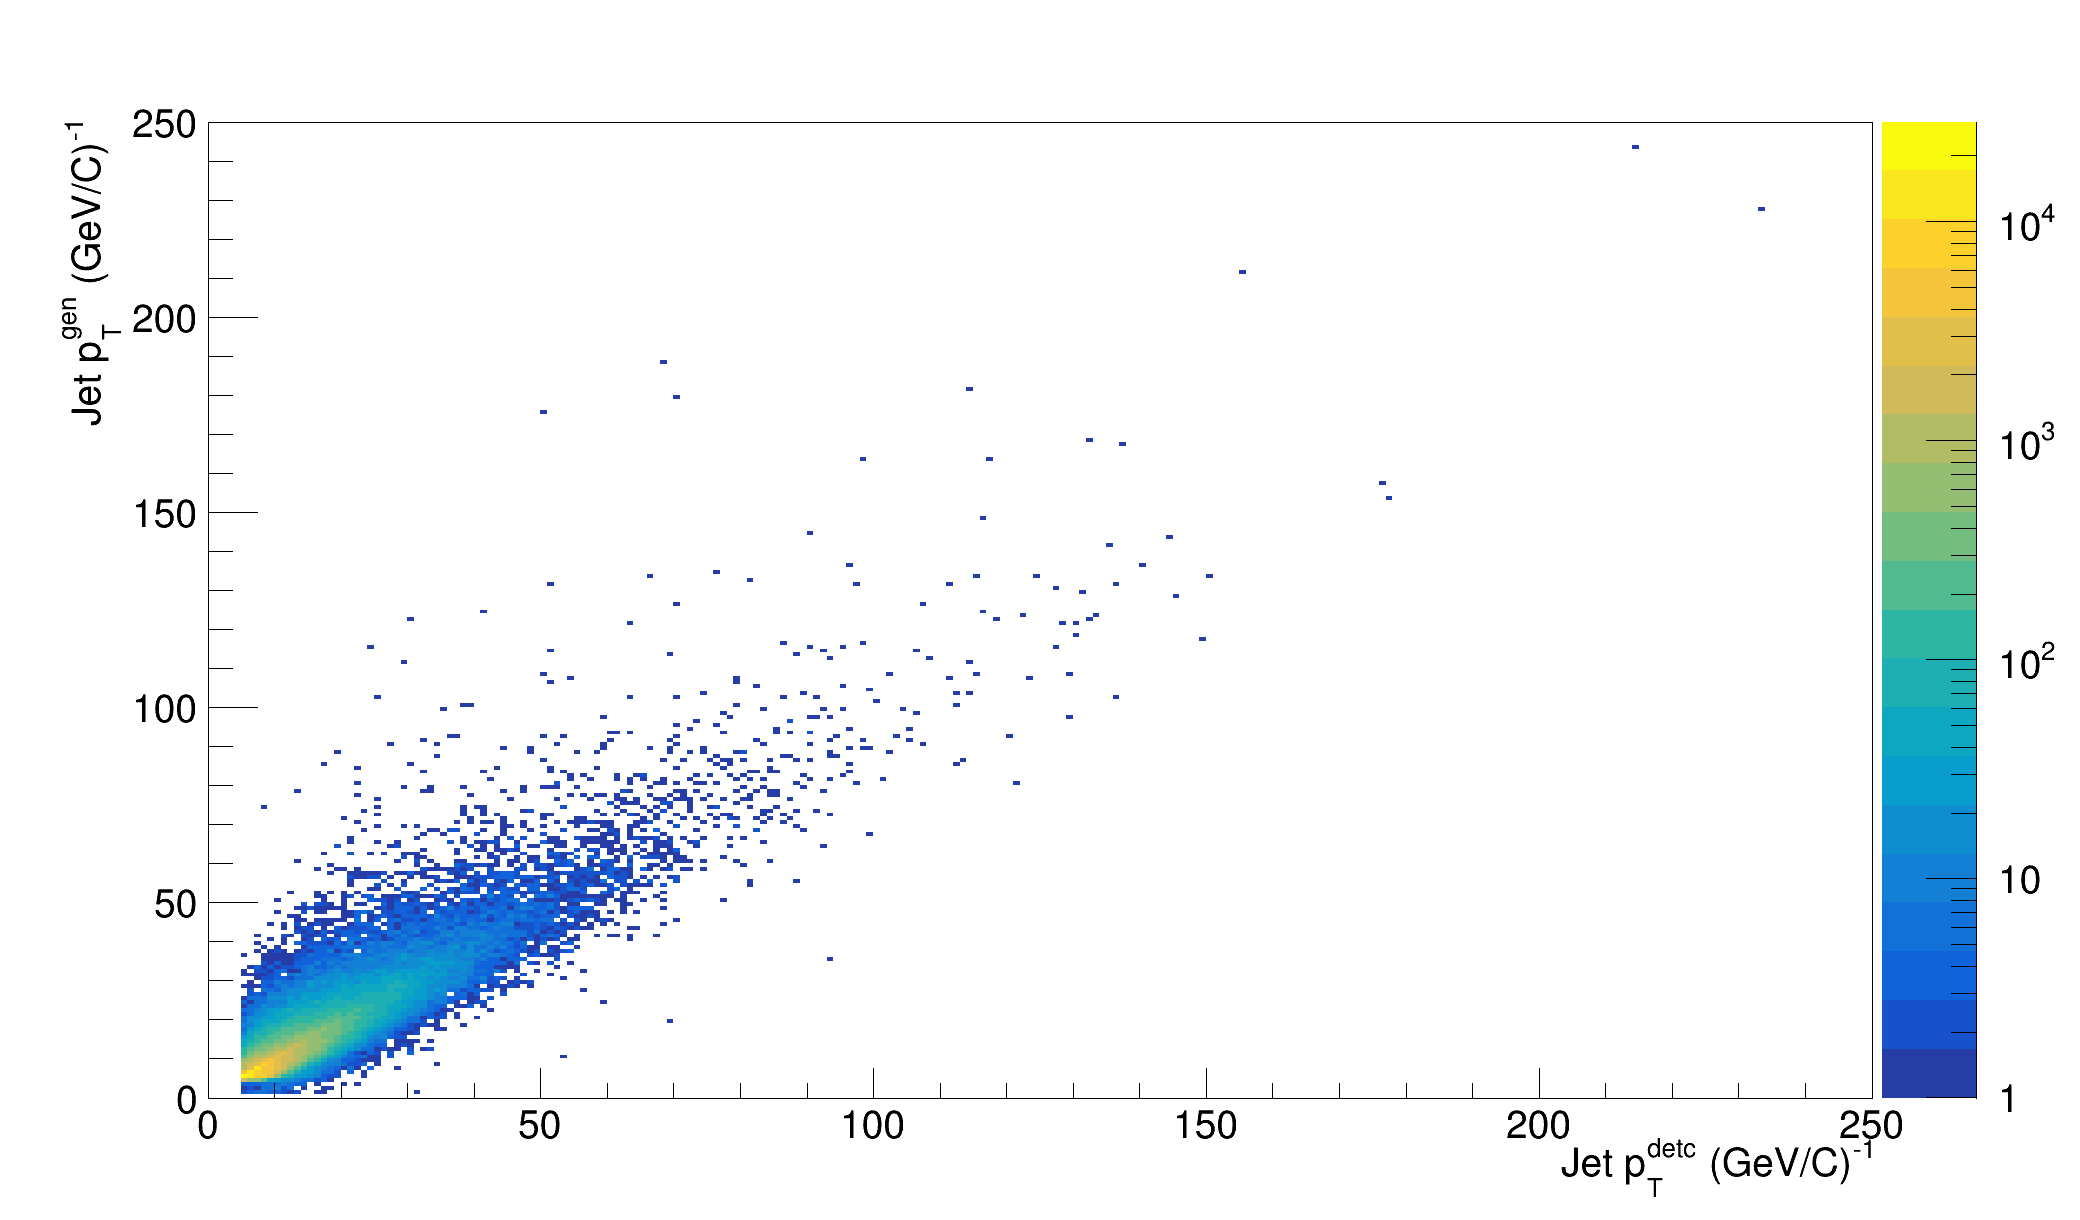
\includegraphics[width=0.5\textwidth]{responseR02} &
    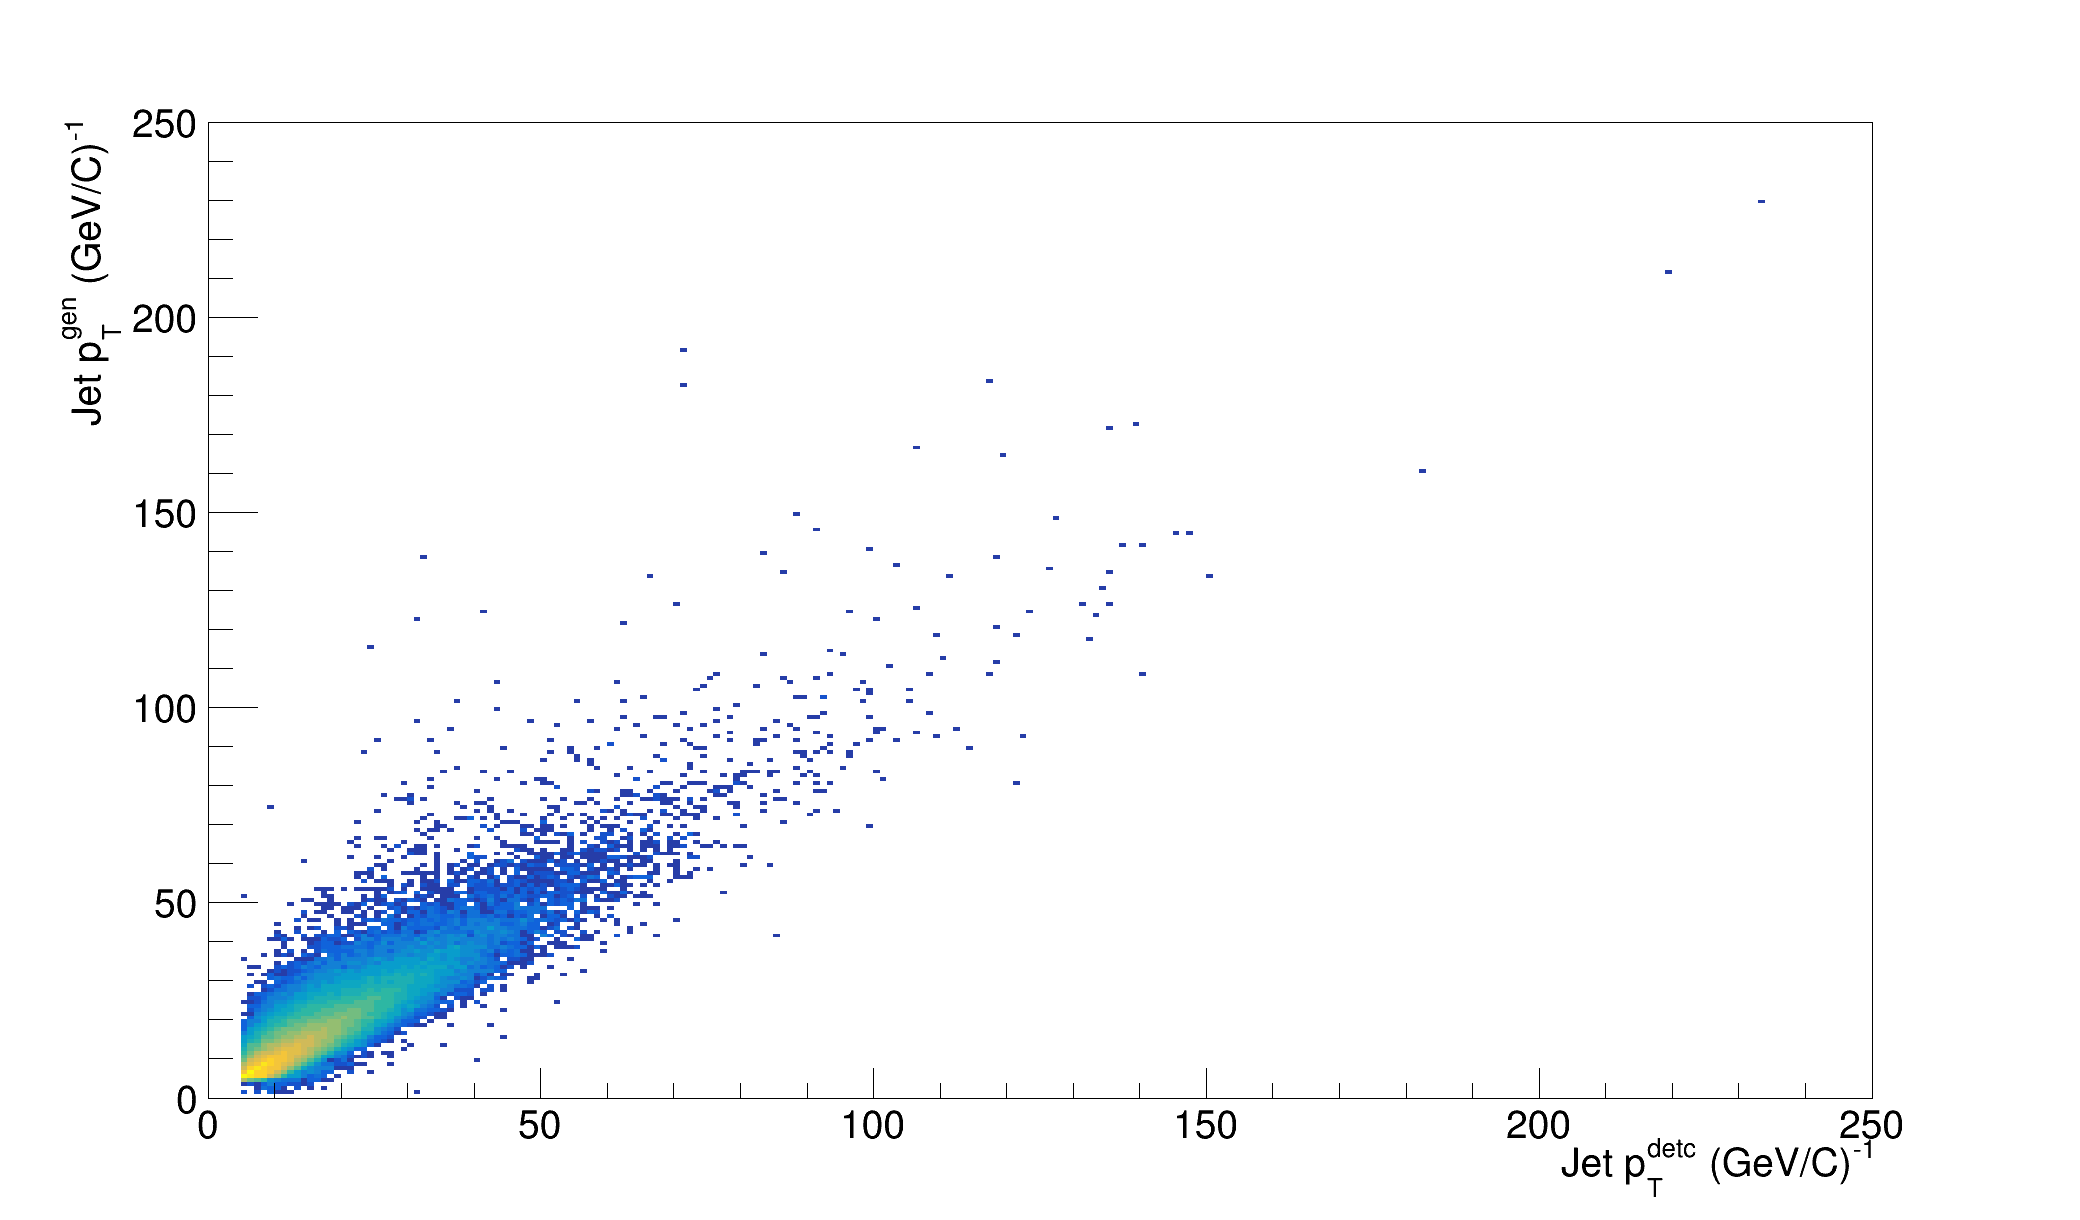
\includegraphics[width=0.5\textwidth]{responseR03}\\
    \multicolumn{2}{c}{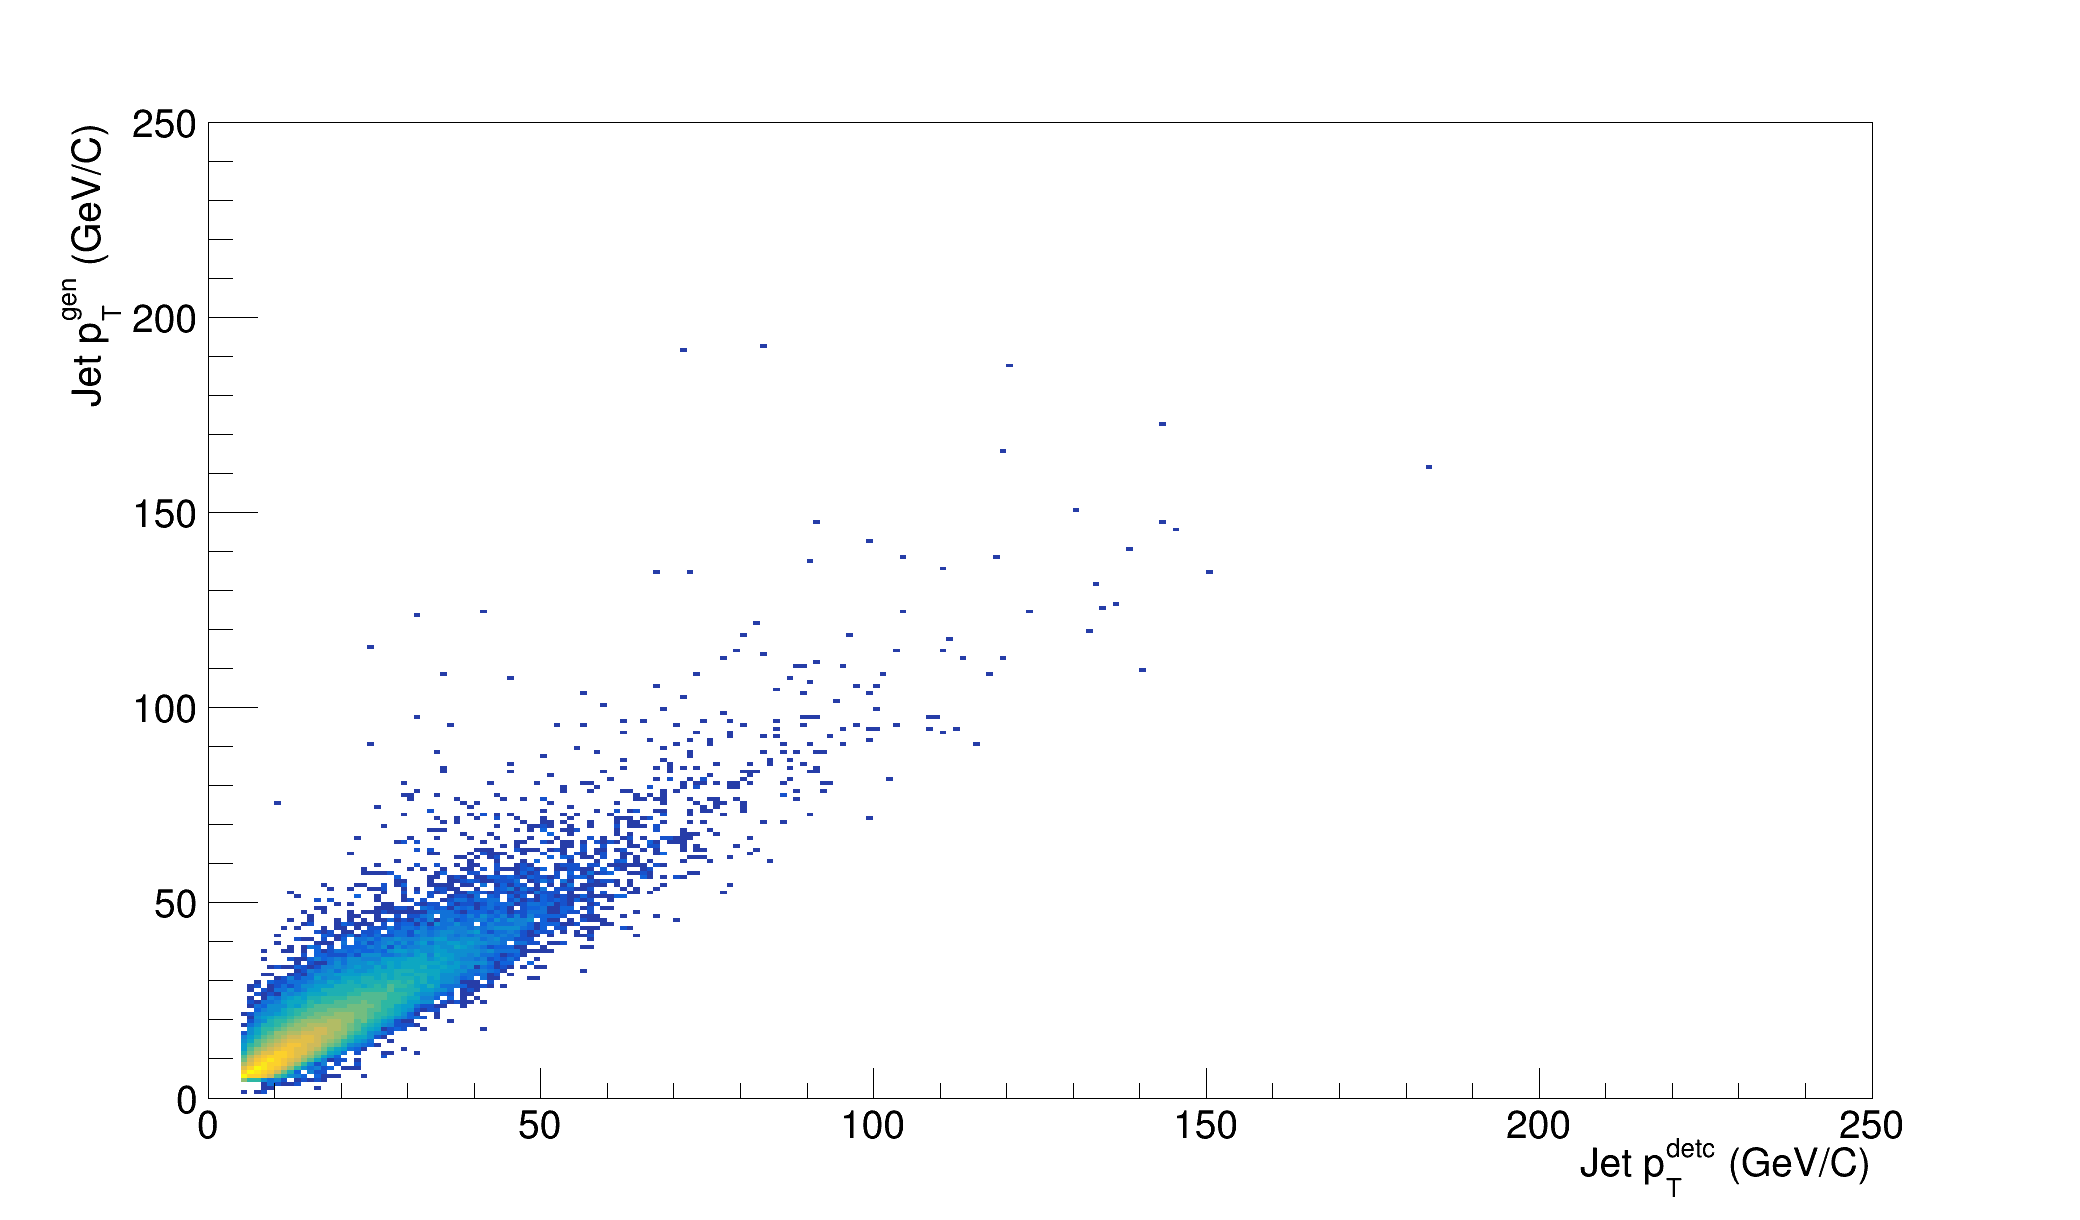
\includegraphics[width=0.5\textwidth]{responseR04}}
\end{array}$
\caption[Response Matrices for R = 0.2, R=0.3, and R = 0.4 jets.]{\label{fig:response}Response Matrices for R = 0.2, R=0.3, and R = 0.4 jets.}
\end{figure*}

Figure \ref{fig:response} shows the response matrices for the R = 0.2 (top left), R = 0.3 (top right), and R = 0.4 (bottom) jets generated with the prescribed manner.  The response matrices display a linear relationship below 50 GeV on both axis and above ~ 100 GeV the matrices are statistics starved.  This is primarily due to the Monte Carlo Pythia and PhoJet data sets generated for the 8 TeV pp run did not model the high-$p_{T}$ triggers associated with the EMCal.  The particle jet finders configured for the response matrices allowed for jet finding down to a 100 MeV jet candidate at the particle level with no constraints on the minimum particle momentum or energy for a constituent.  The detector level jet finders were configured in the same manner as the jet finders configured for the raw jet spectra measurement.  

\subsection{Corrections to Particle Level}

Unfolding was performed using the \verb+RooUnfold+\cite{Adye:2011gm} software package.  Corrections are applied using the bin-by-bin\cite{Cowan:2002in} algorithm. 

\begin{equation}
C_{MC} \big( p_{T}^{low} : p_{T}^{high} \big) =  \frac{  \int^{p_{T}^{high}}_{p_{T}^{low}} dp_{T} \; \frac{dF^{uncorr}_{meas}}{dp_{T}} \times \frac{d^{2}N^{particle}_{MC}/d\eta \, dp_{T}}{d^{2}N^{detector}_{MC}/d\eta \, dp_{T}}  } { \int^{p_{T}^{high}}_{p_{T}^{low}} dp_{T} \; \frac{dF^{uncorr}_{meas}}{dp_{T}} }
\label{eq:binbybin}
\end{equation}

\noindent
where $d^{2}N^{particle}_{MC}/dp_{T} \, d\eta$ is the PYTHIA level inclusive jet spectra, $d^{2}N^{detector}_{MC}/dp_{T} \, d\eta$ is the GEANT 3 level inclusive jet spectra, $dF^{uncorr}_{meas} / dp_{T}$ is a weight function which minimizes the dependence on the two simulation spectra shapes, finally $p_{T}^{low}$ and $p_{T}^{low}$ are the lower and upper bin limits.  Due to the limited statistics derived from the Monte Carlos available the unfolding procedure was stable only in aunfolding the truth level jet spectra for the range: $p_{T,jet} \epsilon \;$ [10 GeV, 120 GeV] for both the raw Min Bias and Emcal triggered data sets.  Due to the  the final truth value for the jet spectra will be reported in this range.



\subsection{Unfolded MB Spectra}

\begin{figure}[h]
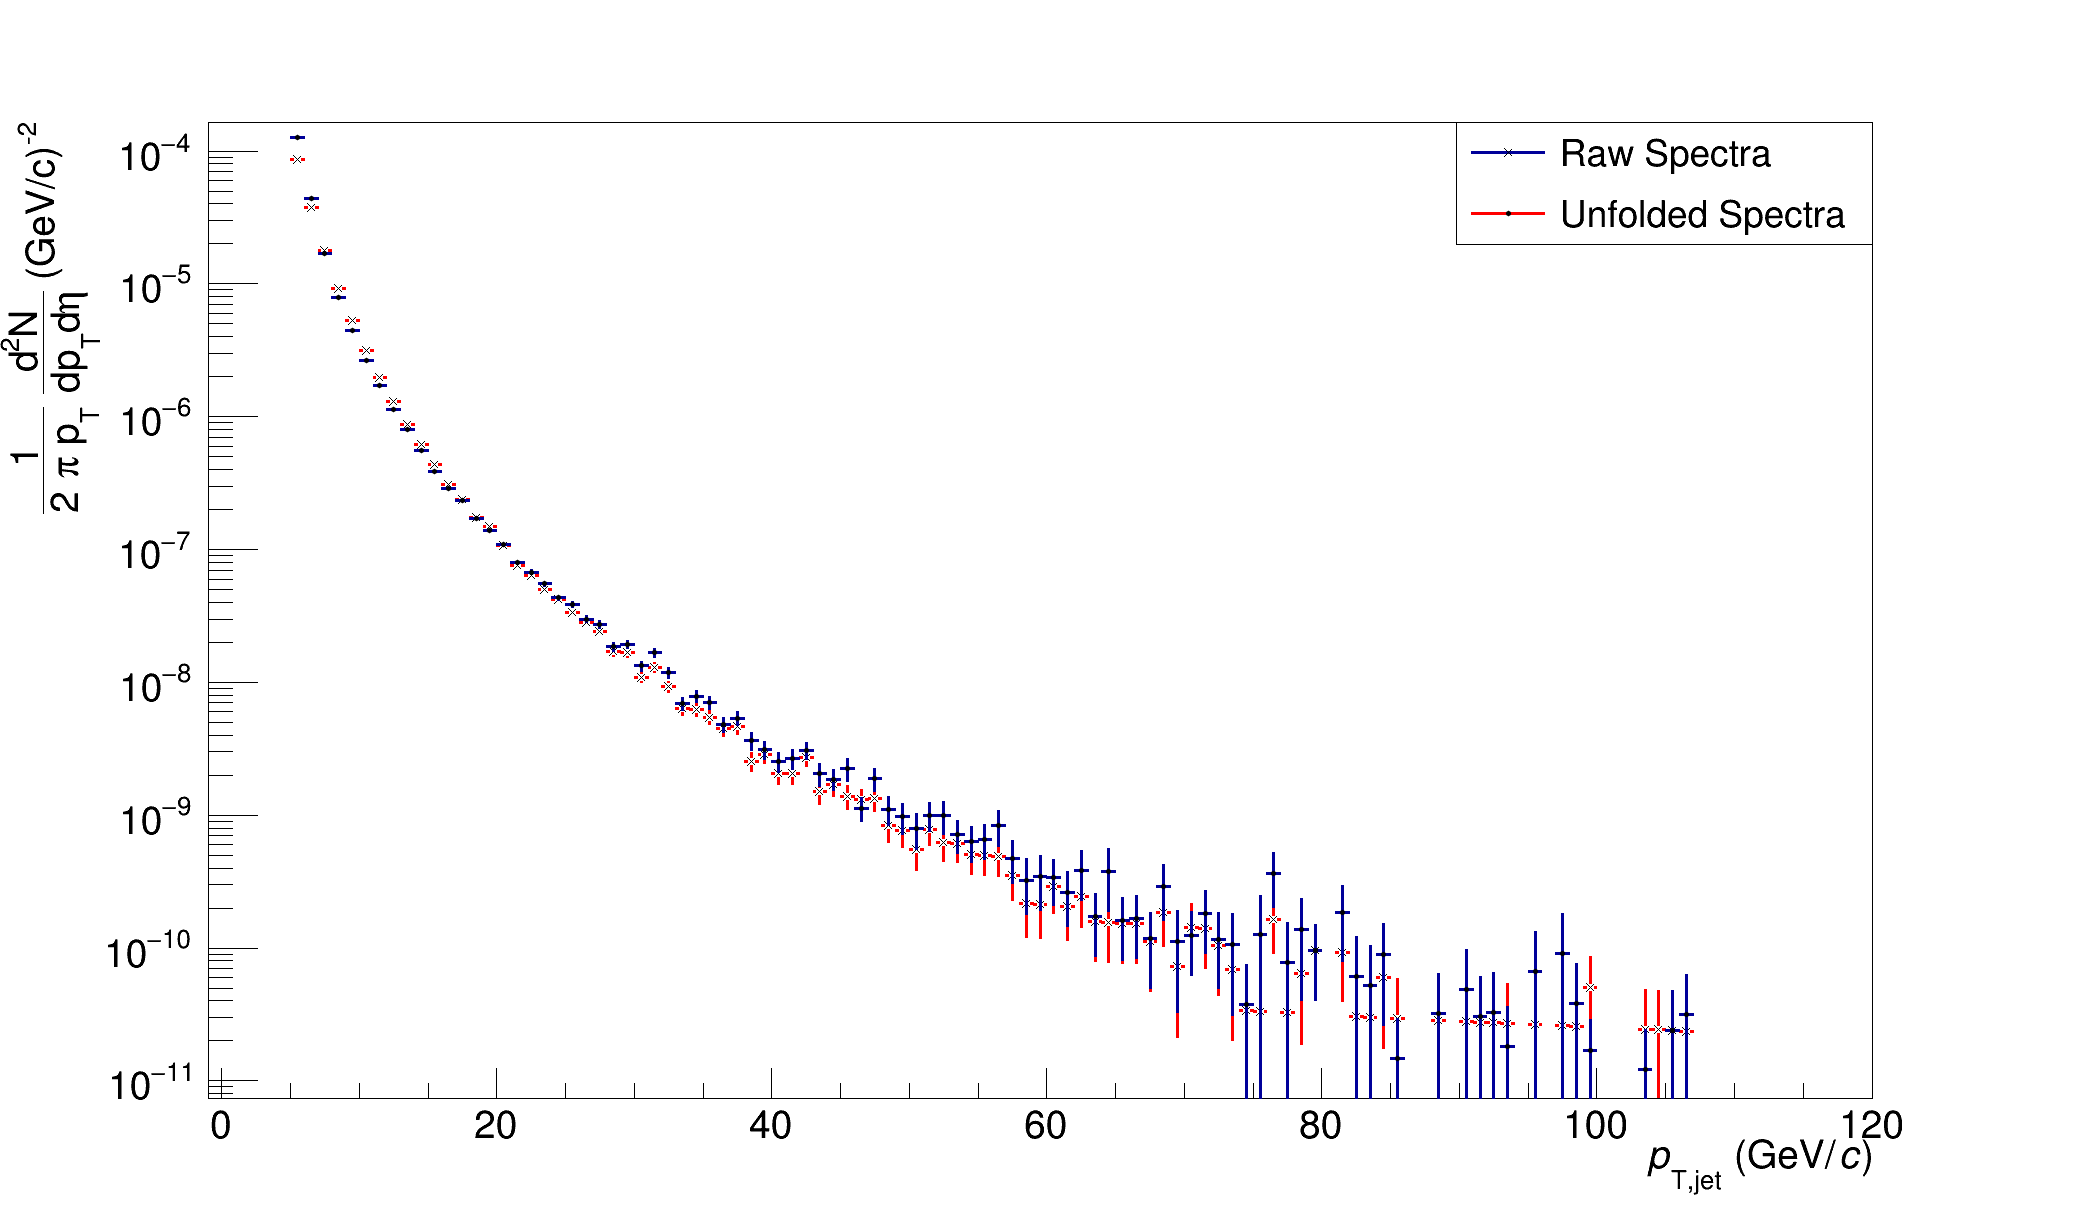
\includegraphics[width=13cm]{RawandUnfoldedSpectraMBR03}
\centering
\caption{Unfolded jet spectra with fine binning for R = 0.3}
\label{fig:Unfoldfine}
\end{figure}

Figure \ref{fig:Unfoldfine} shows an example of the output from the bin-by-bin unfodling with the fine binning for R = 0.3 jets.  It should be noted that at low-$p_{T}$ it was observed that unfolding increased the yield of the spectra while at high-$p_{T} \geq \,$ 40 GeV the yield was decreased for all jet radii in this analysis.  This is most likely due to the lack of statistics in the response matrix.  Once the bin-by-bin unfolding has been performed for the fine binned spectra the output along with the bin-by-bin correction factors ar rebinned using a variable binning between 10 GeV and 120 GeV.

\begin{figure}[h]
\includegraphics[width=10cm]{UnfoldedR02MinBias}
\centering
\caption{Unfolded Min Bias R = 0.2 jet spectra with corrections factors using a variable binning.}
\label{fig:UnfoldvarR02}
\end{figure}

\begin{figure}[h]
\includegraphics[width=10cm]{UnfoldedR03MinBias}
\centering
\caption{Unfolded Min Bias R = 0.3 jet spectra with corrections factors using a variable binning.}
\label{fig:UnfoldvarR03}
\end{figure}

\begin{figure}[h]
\includegraphics[width=10cm]{UnfoldedR04MinBias}
\centering
\caption{Unfolded Min Bias R = 0.4 jet spectra with corrections factors using a variable binning.}
\label{fig:UnfoldvarR04}
\end{figure}


\subsection{Unfolded EMCal Triggered Spectra}
The unfolding procedure is repeated again for the EMCal triggered jet spectra.  The response matrix from the Min Bias sample is used for the bin-by-bin unfolding and performed using a fine binning.  The detector level and particle level jets are configured in the same manner as above and the output from the unfolded triggered specta are reported after rebinning to a variable size over the same kinematic range as the Min Bias sample.

\begin{figure}[h]
\includegraphics[width=10cm]{UnfoldedR02EGAtrigger}
\centering
\caption{Unfolded EMCal triggered R = 0.2 jet spectra with corrections factors using a variable binning.}
\label{fig:UnfoldvarR02EGA}
\end{figure}

\begin{figure}[h]
\includegraphics[width=10cm]{UnfoldedR03EGAtrigger}
\centering
\caption{Unfolded EMCal triggered R = 0.3 jet spectra with corrections factors using a variable binning.}
\label{fig:UnfoldvarR03EGA}
\end{figure}

\begin{figure}[h]
\includegraphics[width=10cm]{UnfoldedR04EGAtrigger}
\centering
\caption{Unfolded EMCal triggered R = 0.4 jet spectra with corrections factors using a variable binning.}
\label{fig:UnfoldvarR04EGA}
\end{figure}

\noindent
Due to the limitations on the response matrix the bin-by-bin unfolding of the EMCal triggered data was only stable up to 120 GeV.  It should be noted that the hump in the EMCal jet spectra is due to the firing threshold of the trigger.  The unfolded Emcal jet spectra was used to estimate the ratio the the jet yields between the Min Bias and triggered data samples, from this point the trigger scaling was calculated.  Due to the lack of a trigger modeled with the 8 TeV Monte Carlo productions the inability to extend the kinematic range of the jet spectras beyond 120 GeV presents a missed oppurtunity in terms of the recorded data from the 8 TeV runs.  In order to address this issue a new Monte Carlo production will need to be requested from the ALICE collaboration.

\subsection{Jet Reconstruction and Matching Efficiency}
In order to quantify the inefficiencies due to unfolding along with inefficencies in the ALICE experiment in reconstructing jets we quantify the jet reconstruction efficiency, $\epsilon_{reco} (p_{T, jet})$, and the jet matching efficiency, $\epsilon_{match} (p_{T, jet})$.

\begin{equation}
 \epsilon_{reco} (p_{T, jet}) = \frac{N_{reco}(p_{T, jet}) }{N_{Truth} (p_{T, jet})}
\label{eq:jetrecoeff}
\end{equation}

\begin{equation}
 \epsilon_{match} (p_{T, jet}) = \frac{N_{match}(p_{T, jet}) }{N_{Truth}(p_{T, jet})}
\label{eq:jetmatchoeff}
\end{equation}

\noindent 
where $N_{reco} (p_{T, jet})$ is the reconstructed jet yield at the detector level per $p_{T}$ bin, $N_{match}(p_{T, jet})$ is the reconstructed jet at the detector level that was matched to a particle level jet per $p_{T}$ bin, and $N_{truth} (p_{T, jet})$ is the truth-level jet yield from the Pythia embedded event per $p_{T}$ bin.  These quantities 

\section{Systematic Uncertainties}

Systematic uncertainties arise due to our limited knowledge of the precise operating conditions and performance of the experiment and also due to any bias in our understanding of how to fundamental model the interactions.  They systematics may therefore be broken into two components: uncertainties to the jet energy scale (JES) which shifts the momentum spectra along the x-axis and uncertainties in the jet yield which shift the spectra along the y-axis.  The systematical and statistical uncertainties presented in this analysis will be presented as errors to the yield of the spectra.  Due to the fact that the $p_{T}$ distribution follows a power law function, $dN/dp_{T} \sim p_{T}^{-5}$ uncertainties in the JES are converted to yield uncertainties by dividing each one by 5.
Due to the low statistics at the highest $p_{T}$ bins in this analysis, uncertainties in this regime my have large statistical fluctuations.  Small ,systematic variations for the input of the jet spectra will have a dramatic effect over sparsely filled bins versus bins with a low granularity.  As such it may be necessary to extrapolate the systematic from a low $p_{T}$ bin to those at the highsest $p_{T}$ range.  The systematics were performed on both the MB and EMCal triggered data samples but no large variation was observed between the two, thus only the uncertainties from the MB sample are shown and are extrapolated to the triggered data.


\subsection{Systematic Uncertainty to Jet Energy Scale}

\subsubsection{Tracking Efficiency}
Corrections for the tracking efficiency were performed by randomly throwing out 5\% of the tracks from each event from the 8 TeV data samples and reperforming jet on the altered data.  All of the inputs for jet finding were maintained.


\begin{figure*}[t!]
$\begin{array}{rl}
    \includegraphics[width=0.5\textwidth]{SysR02_TrkEff} &
    \includegraphics[width=0.5\textwidth]{SysR03_TrkEff}\\
    \multicolumn{2}{c}{\includegraphics[width=0.5\textwidth]{SysR04_TrkEff}}
\end{array}$
\caption[Systematic due to TPC tracking efficiency.]{\label{fig:trkeff}Systematic due to TPC tracking efficiency.}
\end{figure*}

\noindent
Figure \ref{fig:trkeff} shows the systematical uncertainties for R = 0.2 (top left), R = 0.3 (top right), and R = 0.4 (bottom) jets.   

\subsubsection{Hadronic Correction}

\subsubsection{EMCal Clusterization Algorithm}
\subsection{Systematic Uncertainty to Jet Yield}



\subsubsection{Luminosity Uncertainty}

The luminosity of a hadronic collider, $\mathscr{L}$, is given by the expression



\begin{equation}
\mathscr{L} = \frac{R}{\sigma}
\label{eq:xlumdef}
\end{equation}

\noindent
where R is the interaction rate and $\sigma$ is the visible cross section.  Due to the fact that we only measure events within a 10 cm window within the primary vertex region we must scale the total luminosity to that which is delievered within the primary vertex region of the ALICE experiment.  This scale factor is determined by dividing the total number of MB events to those accepted within the 10 cm window.  $N^{tot}_{MB} / N^{10 cm vertex}_{MB}$ = 1.024 from the acceptance criteria held in this analysis.
The luminosity along with its uncertainty were determined during a a special Van der Meer scan run in April of 2012\cite{ALICE-PUBLIC-2017-002}.  The total systematic uncertainty for the minimum bias (MB) trigger were obtained by measuring the visible cross section using the T0 and V0 detectors.  The MB trigger was defined as V0AND which required a hit in both tjhe V0A and V0C.  The cross section was reported as being a combined average for MB with the V0AND as, 

\begin{equation}
\sigma_{V0} = (55.8 \pm 1.2) mb
\label{eq:xlumdef}
\end{equation}

\noindent
with a combined systematic uncertainty of 2.19\% on the visible cross section and 2.60\% on the luminosity. 


\subsection{Total Uncertainty}

A summary of the total systematic errors used in the final analysis.

\begin{tabular}{ |p{5cm}||p{3cm}|p{3cm}|p{3cm}|  }
 \hline
 \multicolumn{4}{|c|}{Systematic Errors} \\
 \hline
 Systematic &R = 0.2 Jets & R = 0.3 Jets& R = 0.4 Jets\\
 \hline
Sensitivity to Clusterization   & AF    &AFG&   004\\
Hadronic Correction&   AX  & ALA   &248\\
Tracking Efficency &AL & ALB&  008\\
Sensitivity to Unfolding&DZ & DZA&  012\\
Momentum Resolution&   AS  & ASM&016\\
Energy Resolution& AND   &020 & 02\\
 Angola& AO  & AGO&024\\
 \hline

\end{tabular}
\noindent

The systematics from the yield and JES are added in quadrater together and this is combined in quardrater with the statistical errors.

\section{Corrected pp jet cross section}


\subsection{Comparisons to pQCD predictions}

\subsection{Jet Cross Sections and Ratios}




    \chapter{Corrections and Systematic Uncertainties} \label{ch:error}

The large amount of data collected for the 8 TeV data set offers a unique chance to explore jet cross-sections using high statistics.   In order to measure the jet double differential cross-section, the following formula is used,

\begin{equation}
	\frac{d^{2} \sigma^{jet}}{d\eta \, dp_{T}} = \frac{1}{\epsilon_{reco}} \frac{A_{trigger}}{\epsilon_{trigger}(p_{T})} \times C_{MC} \times \frac{1}{A} \times \frac{1}{\mathscr{L}_{int}} \times \frac{dN^{2}_{jet}}{dp_{T} \, d\eta}
\label{eq:xsecdef}
\end{equation}

\noindent
where,

\begin{itemize}
  \item $\epsilon_{reco}$ is the efficency for reconstructing the jet in the ALICE detector.
  \item $A_{trigger}$ is the acceptance for EMCal triggered events and $\epsilon_{trigger}(p_{T})$ is the EMCal trigger efficiency.  These factors correct for imperfections in the electronics of the EMCal and the overall factors are equal to one in Min Bias events.
  \item $C_{MC}$ is a correction factor due to detector effects and it allows for comparisons between the ALICE experiment and other experiments or theoretical calculations.  Unfolding is used to determine this factor.
  \item $\mathscr{L}_{int}$ is the integrated luminosity during the period when the data was recorded.
  \item $A$ is the geometrical detector acceptance.
  \item $\frac{dN^{2}_{jet}}{dp_{T} \, d\eta}$ is the inclusive jet momentum spectra.
  
\end{itemize}

By incorporating the additional terms in Equation \ref{eq:xsecdef} we can obtain a fully corrected inclusive jet cross-section that can be compared to theoretical calculations and other experiments.  Further cuts for the geometric acceptance, corrections for detector effects, and efficiency calculations need to be accounted for to create a fully corrected jet result.  This chapter will conclude with a presentation of the systematic errors that are reported with the final jet cross-sections

\section{Raw Jet Spectra}

This analysis measured inclusive jet results for radii between 0.2 and 0.4.  Figures \ref{fig:rawjetR02}, \ref{fig:rawjetR03}, and \ref{fig:rawjetR04} show the raw (uncorrected) $p_{T}$ spectra for inclusive jets from both Min Bias and EMCal triggered data.  It is evident from these figures that the EMCal triggered data greatly extends the kinematic reach of the measured jet spectra, to about 200 GeV/c.  The EMCal data introduces a bias at low-$p_{T}$ as seen in the different distribution shapes.  The next sections of this chapter will discuss corrections to the data including trigger scaling unfolding. 

\afterpage{%
\begin{figure}
\includegraphics[width=\linewidth]{RawR02JetSpectra}
\centering
\caption{Raw inclusive R = 0.2 jet spectra from the 8 TeV Min Bias and EMCal triggered data}
\label{fig:rawjetR02}
\end{figure}

\begin{figure}
\includegraphics[width=\linewidth]{RawR03JetSpectra}
\centering
\caption{Raw inclusive R = 0.3 jet spectra from the 8 TeV Min Bias and EMCal triggered data}
\label{fig:rawjetR03}
\end{figure}

\begin{figure}
\includegraphics[width=\linewidth]{RawR04JetSpectra}
\centering
\caption{Raw inclusive R = 0.4 jet spectra from the 8 TeV Min Bias and EMCal triggered data}
\label{fig:rawjetR04}
\end{figure}

\clearpage
}


\section{Acceptance Correction}
Jet spectra, cross-sections, and ratios of cross-sections are reported over the full azimuth angle and psuedorapidity acceptance in this thesis.  Because jets are constrained to the EMCal a geometric factor was used to correct for the limited acceptance of the detector.  This thesis explored jet radii between 0.1 and 0.5 in order to study the effects of wide angle radiation on jet fragmentation.  Jet measurements in heavy-ion collisions typically use radii of 0.2 to reduce the impact of the high multiplicity.  Due to these geometric corrections the centroid of a jet is constrained to,

\begin{equation}
|\eta_{jet}| \leq 0.7 - R, \; 1.4 + R \leq \phi_{jet} \leq 3.14 -R.
\label{eq:jetconstration}
\end{equation}

\begin{equation}
A(p_{T}) = \frac{(1.4 - 2R) \times (1.745 - 2R)}{2 \pi}.
\label{eq:acceptance}
\end{equation}

For jets between R = 0.1 through R = 0.5 the following jet acceptance corrections were used, see Table 5.2.

\begin{table}[hb]
\label{tab:AcceptanceFactor}
\begin{center}
\caption{EMCal jet acceptance for radii 0.1 - 0.5.}
\begin{tabular}[b]{|c|c|c|}
	\hline
	Jet R & $ A $ \\ \hline
	0.1 & 0.296 \\ \hline
	0.2 & 0.214\\ \hline
	0.3 & 0.146\\ \hline
	0.4 & 0.091\\ \hline
	0.5 & 0.048\\ \hline
\end{tabular}
\end{center}

\end{table}

\section{EMCal Triggered Data}

As discussed in Chapter \ref{ch:alice}, the ALICE detector is unable to record all events that occur in the experiment.   The use of a trigger allows for events with rare processes to be saved with a high efficiency and analyzed.  The high-$p_{T}$ EMCal trigger used for the 8 TeV data extends the kinematic reach of the spectra and the sample of jets from the data.  This thesis looked at the two primary Level-1 triggers configured for the EMCal, the jet trigger and the gamma trigger\cite{Bourrion:2010js}.  Although both of the Level-1 triggers were investigated in this analysis, only the gamma trigger was ultimately used for the final jet cross-sections and spectra.  

The jet trigger is a patch consisting of 32 x 32 EMCal towers, roughly the same size as a R = 0.3 jet.  The patch samples all possible tower conditions until the patch meets the minimum predefined energy threshold.  Once this threshold is surpassed the event is recorded and tagged as a jet triggered event.  A similar procedure is followed for the gamma trigger, but with a smaller patch region of 4 x 4 towers and a different energy threshold.  

The bump at low-$p_{T}$ seen in Figures \ref{fig:rawjetR02} - \ref{fig:rawjetR04} is the trigger turn on curve and the peak corresponds to the trigger threshold for the EGA trigger.  A jet in the EMCal acceptance should fire the jet trigger and the gamma should fire due to the presence of a photon or electron. The EMCal triggered events have a higher yield of jets compared to the Min Bias spectra. The triggered data is downscaled, this corrects the enhancement and makes the triggered data equivalent to the Min Bias data.  

The triggered data also needs to be corrected by reconstructing the jet that fired the jet trigger.  This analysis was concerned with analyzing jets that fired the trigger and removing any bias to processes outside of jet production. Therefore jets were matched to the trigger patch.  In order to only correct jets that fired a trigger in the EMCal the following procedure was implemented.  First both the jet and gamma trigger patches were reconstructed offline.  Next the energy thresholds were set for each trigger.  Then the centroid of the trigger was found by finding the center-of-mass for each reconstructed patch in $\eta$ and $\phi$.  After all patches were reconstructed and their weighted centroids found, each patch was geometrically matched to the jet centroid.  The geometrical matching requirement followed a simple quadratic relationship which constrained the center of the trigger to inside the jet radius,

\begin{equation}
\sqrt{ ( \phi_{jet} - \phi_{EMCal patch} )^{2} + ( \eta_{jet} - \eta_{EMCal patch} )^{2}}  \leq R_{jet} .
\label{eq:triggermatch}
\end{equation}

\begin{figure}[h]
\includegraphics[width=10cm]{DistanceJetEJER02}
\centering
\caption{Distance to closest reconstructed jet patch to R = 0.2 jet with the EMCal triggered data.}
\label{fig:DisJetEJE}
\end{figure}

\begin{figure}[h]
\includegraphics[width=10cm]{DistanceJetEGAR02}
\centering
\caption{Distance to closest reconstructed gamma patch to R = 0.2 jet with EMCal triggered data.}
\label{fig:DisJetEGA}
\end{figure}

\noindent
If a match between the gamma patch and a jet is made, the jet is flagged as causing the triggered event.  Figures \ref{fig:DisJetEJE} and \ref{fig:DisJetEGA} show the distance between a reconstructed jet and its closest reconstructed EMCal trigger patch for R = 0.2 jets using the triggered data  Since a trigger patch may be fired if two or more jets are within the geometric area of the trigger patch this could lead to double counting.  In order to correct for this, the jet spectra from the triggered data is scaled by the number of triggers, $N_{trig}$, fired that fell within the jet.  We see that with the gamma trigger that the peak of the distribution was within the jet radius of R = 0.2, while with the jet trigger the distribution is more uniformly distributed. 

Once this correction was implemented, the triggered data were then downscaled in order to combine it with the Min Bias data.  The downscale correction factors, shown in Figure \ref{fig:EMCalDownScale}, were obtained by taking the ratio of the EMCal jet spectra to the Min Bias jet spectra and fitting the plateau region to a line.  Below $\sim$40 GeV/\textit{c}, the efficiency in the triggered data is changing rapidly and hard to determine.  Due to the Min Bias data being sufficient in measuring the low kinematic range of the jet spectra the downscaled EMCal data is used at 40 GeV/\textit{c} and above.  The scale factors seen in Figure \ref{fig:EMCalDownScale} were obtained after the corrections to the Monte Carlo models were done.


\begin{figure*}[t!]
$\begin{array}{rl}
    \includegraphics[width=0.5\textwidth]{R02TriggerYields} &
    \includegraphics[width=0.5\textwidth]{R03TriggerYields}\\
    \multicolumn{2}{c}{\includegraphics[width=0.5\textwidth]{R04TriggerYields}}
\end{array}$
\caption[EMCal triggered data correction factors for R=0.2, R=0.3, and R=0.4 jets.]{\label{fig:EMCalDownScale}EMCal triggered data correction factors for R=0.2, R=0.3, and R=0.4 jets.}
\end{figure*}
 

\section{Particle Level Corrections}

The reconstructed jet $p_{T}$ has a number of detector effects present in the measurement.  These effects include such things as:

\begin{itemize}
\item Tracking inefficiencies from the TPC and ITS.
\item Missing jet energy components from long-lived particles, such as the $K^{0}_{L}$ and neutron, that are cut by the EMCal timing requirement.
\item TPC track $p_{T}$ and EMCal cluster energy resolutions.
\item Hadronic corrections to the EMCal cluster spectrum.
\item Material loss in the detectors.
\end{itemize}

\noindent
The magnitude of any one of these inefficencies may be small but together they can contribute to large discrepencies.  `Bin-by-bin' corrections is a method by which these detector effects are removed from the raw inclusive jet spectra so that a `true' jet spectra may be obtained and compared with theoretical calculations or other experimental results.  

In order to correct a jet spectra, it is necessary to generate a response matrix that simulates the described effects above.  In order to generate the response matrix, a PYTHIA generated event is embedded into a GEANT simulation of the ALICE detector.  Each LHC period has a unique GEANT simulation produced for it to account for changes in the detector performance.  The differences in the simulations take into account all the hot and dead sectors for the subdetectors, along with their calibrated performance during that specified data taking period.  The bin-by-bin corrections used in this analysis were taken from the PYTHIA plus GEANT simulations produced from the ALICE collaboration.

\subsubsection{Response Matrix}
The output from the PYTHIA portion of the simulation contains all the final state hadrons, regardless of them being detected in the experiment.  This is known as the particle level.  The particle-level PYTHIA jets are constructed from the primary particles generated via PYTHIA.  After the particle-level jet passes through the GEANT simulation of ALICE we obtain the detector-level jets with all detector inefficiencies incorporated.
The response matrix is constructed by geometrically matching particle-level jets to detector-level.  The particle-level jet centroid ($\phi_{part}$,$\eta_{part}$) is matched to the detector-level jet centroid ($\phi_{det}$,$\eta_{det}$) via a constraint on the displaced distance between the two jet centroids.  This distance was constrained to: $\Delta  R = \sqrt{(\phi_{part} - \phi_{det})^{2} + (\eta_{part} - \eta_{det})^{2}} \leq 0.25 \; $.  Once a jet was matched at the detector-level to a jet generated from the particle-level the response matrix was incremented by jet $p_{T}$ at both the detector and Monte Carlo levels.



\begin{figure}[h]
\includegraphics[width=\linewidth]{responseR02}
\centering
\caption{Response matrix for R = 0.2 jets.}
\label{fig:rawjetR02}
\end{figure}

Figure \ref{fig:response} shows the response matrices for the R = 0.2 jets with the PYTHIA Min Bias sample.  The y-axis shows the jet $p_{T}$ at the particle-level from PYTHIA and the x-axis shows the jet $p_{T}$ after it has been propagated throught the GEANT simulation of ALICE.  The response matrix shows a slight linear relationship below 50 GeV on both axis and show that above $\sim$100 GeV the matrix lack statistics.  This is primarily due to the Monte Carlo PYTHIA and PHOJET events simulated for the 8 TeV pp run did not model the high-$p_{T}$ EMCal triggers.  The jet finder was configured for a minimum jet energy of 100 MeV and no minimum energy requirement at the particle-level.  The detector-level jet finders were configured in the same manner as they were for the raw jet spectra measurement.  Response matrices with detector-level and particle-level radii of R = 0.3 and R = 0.4 were generated and used to perform corrections on the R = 0.3 and R = 0.4 jet spectra, respectively. 

\subsubsection{Corrections to particle-level}

Corrections were performed using the \verb+RooUnfold+\cite{Adye:2011gm} software package.  RooUnfold can perform corrections using the bin-by-bin method, it can also perform unfolding using either the Bayesian or singular value decomposition.  particle-level corrections were initially attempted using either using either Bayesian or Singular Value Decomposition unfolding but both were unstable due to low statistics. Corrections were applied using the bin-by-bin\cite{Cowan:2002in} algorithm. 

\begin{equation}
C_{MC} \big( p_{T}^{low} : p_{T}^{high} \big) =  \frac{  \int^{p_{T}^{high}}_{p_{T}^{low}} dp_{T} \; \frac{dF^{uncorr}_{meas}}{dp_{T}} \times \frac{d^{2}N^{particle}_{MC}/d\eta \, dp_{T}}{d^{2}N^{detector}_{MC}/d\eta \, dp_{T}}  } { \int^{p_{T}^{high}}_{p_{T}^{low}} dp_{T} \; \frac{dF^{uncorr}_{meas}}{dp_{T}} }
\label{eq:binbybin}
\end{equation}

\noindent
where $d^{2}N^{particle}_{MC}/dp_{T} \, d\eta$ is the PYTHIA particle-level inclusive jet spectra, $d^{2}N^{detector}_{MC}/dp_{T} \, d\eta$ is the GEANT detector-level inclusive jet spectra, $dF^{uncorr}_{meas} / dp_{T}$ is a weight function which minimizes the dependence on the two simulation spectra shapes, and finally $p_{T}^{low}$ and $p_{T}^{high}$ are the lower and upper bin limits.  Due to the limited statistics derived from the availabe Monte Carlos, the bin-by-bin corrections were stable for a jet momentum range of: $p_{T,jet} \, \, \epsilon \;$ [10 GeV, 120 GeV] for both the raw Min Bias and EMCal triggered data sets.  

\subsubsection{Corrected Jet Spectra}


At low-$p_{T}$ it was observed that unfolding increased the yield of the spectra while at high-$p_{T} \geq \,$ 40 GeV the yield was decreased for all jet radii in this analysis.  This is most likely due to the lack of statistics in the response matrix.  Once the bin-by-bin corrections were performed for the fine binned spectra the output along with the bin-by-bin correction factors were obtained between 10 GeV and 120 GeV, these corrected spectra are shown in Figures \ref{fig:JetSpecCorrR02}, \ref{fig:JetSpecCorrR03}, and \ref{fig:JetSpecCorrR04}.

\afterpage{%

\begin{figure}
\includegraphics[width=\linewidth]{UnfoldedR02MinBias}
\centering
\caption{R = 0.2 bin-by-bin corrected Min Bias jet spectra.}
\label{fig:JetSpecCorrR02}
\end{figure}

\begin{figure}
\includegraphics[width=\linewidth]{UnfoldedR03MinBias}
\centering
\caption{R = 0.3 bin-by-bin corrected Min Bias jet spectra.}
\label{fig:JetSpecCorrR03}
\end{figure}

\begin{figure}
\includegraphics[width=\linewidth]{UnfoldedR04MinBias}
\centering
\caption{R = 0.4 bin-by-bin corrected Min Bias jet spectra.}
\label{fig:JetSpecCorrR04}
\end{figure}

\clearpage
}



\subsubsection{Unfolded EMCal Triggered Spectra}
The bin-by-bin procedure was repeated again for the EMCal triggered jet spectra.  The response matrix from the Min Bias sample was used for the bin-by-bin unfolding.  The detector-level and particle-level jets were configured in the same manner as above and the output from the unfolded triggered spectra are reported over the same kinematic range as the Min Bias spectra, as seen in Figures \ref{fig:JetSpecCorrEMCR02}, \ref{fig:JetSpecCorrEMCR03}, and \ref{fig:JetSpecCorrEMCR04}.


\afterpage{%

\begin{figure}
\includegraphics[width=\linewidth]{UnfoldedR02EGAtrigger}
\centering
\caption{R = 0.2 bin-by-bin corrected EMCal triggered jet spectra.}
\label{fig:JetSpecCorrEMCR02}
\end{figure}

\begin{figure}
\includegraphics[width=\linewidth]{UnfoldedR03EGAtrigger}
\centering
\caption{R = 0.3 bin-by-bin corrected EMCal triggered jet spectra.}
\label{fig:JetSpecCorrEMCR03}
\end{figure}

\begin{figure}
\includegraphics[width=\linewidth]{UnfoldedR04EGAtrigger}
\centering
\caption{R = 0.4 bin-by-bin corrected EMCAL triggered jet spectra.}
\label{fig:JetSpecCorrEMCR04}
\end{figure}

\clearpage
}

Due to the limitations of the response matrix, the bin-by-bin corrections of the EMCal triggered data were only stable up to 120 GeV.  Again, it should be noted that the hump in the EMCal jet spectra is due to the firing threshold of the trigger.  The corrected EMCal jet spectra were used to estimate the ratio that the jet yields between the Min Bias and triggered data samples, from this point the trigger scaling was calculated.  

\section{Jet Reconstruction and Matching Efficiency}
In order to quantify the inefficiencies due to unfolding along with the inefficiencies in the ALICE experiment in reconstructing jets, we quantify the jet reconstruction efficiency, $\epsilon_{reco} (p_{T, jet})$, and the jet matching efficiency, $\epsilon_{match} (p_{T, jet})$.

\begin{equation}
 \epsilon_{reco} (p_{T, jet}) = \frac{N_{reco}(p_{T, jet}) }{N_{Truth} (p_{T, jet})}
\label{eq:jetrecoeff}
\end{equation}

\begin{equation}
 \epsilon_{match} (p_{T, jet}) = \frac{N_{match}(p_{T, jet}) }{N_{Truth}(p_{T, jet})}
\label{eq:jetmatchoeff}
\end{equation}

\noindent 
where $N_{reco} (p_{T, jet})$ is the reconstructed jet yield at the detector-level per $p_{T}$ bin, $N_{match}(p_{T, jet})$ is the reconstructed jet at the detector-level that was matched to a particle-level jet per $p_{T}$ bin, and $N_{truth} (p_{T, jet})$ is the particle-level jet yield from the PYTHIA embedded event per $p_{T}$ bin.  

The $N_{truth} (p_{T, jet})$ were obtained by running Fastjet on PYTHIA events with no constituent $p_{T}$ cut, while $N_{match}(p_{T, jet})$ and $N_{reco} (p_{T, jet})$ had the same kinematic cuts as the data driven analysis mentioned earlier in this chapter.  The particle-level jets contained no geometric acceptance cut in order to account for jets that may have been reconstructed at the detector-level, but had no match to a particle-level jet because part of the particle-level jet was outside the EMCal acceptance.  The spectra were corrected by the efficiencies after the bin-by-bin corrections were performed.  The correction factors are shown in Figures \ref{fig:JetMatcheff} and \ref{fig:JetRecoeff}.

\begin{figure*}[t!]
$\begin{array}{rl}
    \includegraphics[width=0.5\textwidth]{Ematch_R02} &
    \includegraphics[width=0.5\textwidth]{Ematch_R03}\\
    \multicolumn{2}{c}{\includegraphics[width=0.5\textwidth]{Ematch_R04}}
\end{array}$
\caption[Jet reconstruction efficiency for jets between R = 0.2 and R = 0.4. ]{\label{fig:JetMatcheff}Jet matching efficiency for jets between R = 0.2 (top left), R = 0.3 (top right), and R = 0.4 (bottom).}
\end{figure*}

\begin{figure*}[t!]
$\begin{array}{rl}
    \includegraphics[width=0.5\textwidth]{Ereco_R02} &
    \includegraphics[width=0.5\textwidth]{Ereco_R03}\\
    \multicolumn{2}{c}{\includegraphics[width=0.5\textwidth]{Ereco_R04}}
\end{array}$
\caption[Jet reconstruction efficiency for jets between R = 0.2 and R = 0.4.]{\label{fig:JetRecoeff}Jet reconstruction efficiency for jets between R = 0.2 (top left), R = 0.3 (top right), and R = 0.4 (bottom)}
\end{figure*}


.

\section{Systematic Uncertainties}

The systematics may be broken into two categories: uncertainties in the jet energy scale (JES) which shift the momentum spectra along the momentum axis, and uncertainties in the jet yield, which shift the spectra along the spectra/cross-section axis.  The total systematic uncertainty to the jet cross-section is obtained by adding each contributing systematic together in quadrature.  The systematic and statistical uncertainties presented in this analysis will be reported as uncertainties to the yield of the spectra.  

In general the systematic uncertainties were obtained by using small variations for the analysis cuts and parameters used in this analysis.  A feature in some of the following uncertainties is the wide statistical fluctuations seen at the highest jet $p_{T}$ bins.  A small change in a input parameter can cause a relatively large flow into and out of a high granularity bin, which does not represent a systematic uncertainty.  In order to obtain the systematic at the highest jet $p_{T}$ bins it was necessary to extrapolate the uncertainty from the low $p_{T}$ range.  There is a degree of arbitrariness to this procedure and at times the uncertainty from a given systematic is assigned a conservative value.  

\subsubsection{Systematic Uncertainty to Jet Energy Scale}

The following sections present and discuss the uncertainties caused by shifts to the JES. 

\subsubsection{Tracking Efficiency Sensitivity}
Only a fraction of charged tracks generated by the hard scattering of two protons will be detected in the TPC due to its finite track efficiency.  Uncertainties in the efficiency of the TPC were studied and found to account for a 5\% discrepancy\cite{Abelev:2013ala}.  In order to obtain the uncertainty on the JES due to the tracking efficiency, this analysis was repeated while throwing out 5\% of the tracks from each event and remeasuring the jet spectra.  Once this new jet spectrum was generated, it was corrected using the bin-by-bin corrections and the ratio of this new spectra was taken with the original spectra to gauge the uncertainty from the tracking efficiency.


\begin{figure*}[t!]
$\begin{array}{rl}
    \includegraphics[width=0.40\textwidth]{SysR02_TrkEff} &
    \includegraphics[width=0.40\textwidth]{SysR03_TrkEff}\\
    \multicolumn{2}{c}{\includegraphics[width=0.40\textwidth]{SysR04_TrkEff}}
\end{array}$
\caption[Systematic due to TPC tracking efficiency.]{\label{fig:trkeff}Systematic due to TPC tracking efficiency; R = 0.2 \textit{(top left)}, R = 0.3 \textit{(top right)}, R = 0.4 \textit{(bottom)}.}
\end{figure*}


Figure \ref{fig:trkeff} shows the systematical uncertainties for R = 0.2, R = 0.3, and R = 0.4 jets.  From the figures a 10\% systematic was assigned to R = 0.2 and R = 0.3 jets, while a 15\% systematic uncertainty was given to R = 0.4 jets for this analysis.

\subsubsection{Hadronic Correction}

\begin{figure*}[t!]
$\begin{array}{rl}
    \includegraphics[width=0.40\textwidth]{SysR02_F07} &
    \includegraphics[width=0.40\textwidth]{SysR03_F07}\\
    \multicolumn{2}{c}{\includegraphics[width=0.40\textwidth]{SysR04_F07}}
\end{array}$
\caption[Systematic due to Hadronic correction.]{\label{fig:hadeff}Systematic due to hadronic correction efficiency; R = 0.2 \textit{(top left)}, R = 0.3 \textit{(top right)}, R = 0.4 \textit{(bottom)}.}
\end{figure*}

The uncertainty in the JES due to the hadronic correction applied to EMCal clusters was measured by changing the nominal value of $f_{sub} = 1$ in equation \ref{eq:HadCorr} to 0.7 and the analysis chain is repeated.  Figure \ref{fig:hadeff} shows the ratio of the new spectra with the original, and the uncertainty due to the hadronic correction was around 5\% for all jet radii.

\subsubsection{Sensitivity to EMCal Clusterization Algorithm}
The clusterization algorithm, discussed in Chapter \ref{ch:data}, limits the number of EMCal towers in a cluster to a maximum of nine.  In order to test the sensitivity the JES has to the clusterization algorithm, a different algorithm was chosen and a new spectra was generated.  The new algorithm is similar to the original algorithm with the exception that the total size of the cluster is forced to be smaller then nine towers.  Similar to the other systematics presented, we see large fluctuations at high-$p_{T}$ due to sparsely field binning.  

\begin{figure*}[t!]
$\begin{array}{rl}
    \includegraphics[width=0.40\textwidth]{SysR02_v1Clusterization} &
    \includegraphics[width=0.40\textwidth]{SysR03_v1Clusterization}\\
    \multicolumn{2}{c}{\includegraphics[width=0.40\textwidth]{SysR02_v1Clusterization}}
\end{array}$
\caption[Systematic due to clusterization algorithm.]{\label{fig:cluseff}Systematic due to EMCal clusterization algorithm; R = 0.2 \textit{(top left)}, R = 0.3 \textit{(top right)}, R = 0.4 \textit{(bottom)}.}
\end{figure*}

Figure \ref{fig:cluseff} shows the systematic uncertainty to the clusterization for each of the jet radii.  At low-$p_{T}$ I assigned an uncertainty of between 1\% and 3\% for a given jet radii.  At high-$p_{T}$ I assigned a 5\% for R = 0.2 and 10\% uncertainty for R = 0.3 and R=0.4 jets to help account for the statistical fluctuations.

\subsubsection{Systematic Uncertainty to Jet Yield}

The following sections discuss the systematic uncertainties affecting the jet yield.

\subsubsection{Track $p_{T}$ Resolution}

\begin{figure}[h]
\includegraphics[width=8cm]{trackcovmatrix}
\centering
\caption{Inclusive TPC track momentum resolution, Min Bias 8 TeV.}
\label{fig:trackpcovmatrix}
\end{figure}

\begin{figure*}[t!]
$\begin{array}{rl}
    \includegraphics[width=0.40\textwidth]{SysR02_PtReso} &
    \includegraphics[width=0.40\textwidth]{SysR03_PtReso}\\
    \multicolumn{2}{c}{\includegraphics[width=0.40\textwidth]{SysR04_PtReso}}
\end{array}$
\caption[Systematic due to $P_{T}$ resolution.]{\label{fig:pTeff}$P_{T}$ resolution systematic; R = 0.2 \textit{(top left)}, R = 0.3 \textit{(top right)}, R = 0.4 \textit{(bottom)}.}
\end{figure*}

\noindent
The momentum resolution of the TPC is estimated using the covariance matrix generated from the Kalman filtering\cite{Fruhwirth:1987fm} pad signal on the TPC read-out region.  Figure \ref{fig:trackpcovmatrix} shows that for the vast majority of the $p_{T}$ range in this analysis the  momentum resolution is below 3\%.  To estimate the systematic uncertainty due to the $p_{T}$ resolution, tracks are smeared by 3\% in $p_{T}$ and the variation between the new and original spectra are used to estimate the uncertainty.  From the generated plots seen in Figure \ref{fig:pTeff} the uncertainties were below 5\% for all jet radii.

\subsubsection{Cluster Energy Resolution}

\begin{figure*}[t!]
$\begin{array}{rl}
    \includegraphics[width=0.40\textwidth]{SysR02_EReso} &
    \includegraphics[width=0.40\textwidth]{SysR03_EReso}\\
    \multicolumn{2}{c}{\includegraphics[width=0.40\textwidth]{SysR04_EReso}}
\end{array}$
\caption[Systematic due to energy resolution.]{\label{fig:Eeff}Systematic due to the energy resolution; R = 0.2 \textit{(top left)}, R = 0.3 \textit{(top right)}, R = 0.4 \textit{(bottom)}.}
\end{figure*}

Similar to the $p_{T}$ resolution, the uncertainty due to the EMCal energy resolution is done by smearing the energy of the clusters by the energy resolution function measured from the test beam, and seen in Figure \ref{fig:Eeff}.  The ratio of the spectra with the smear versus the original spectra are show in Figure \ref{fig:Eeff}. The uncertainties for the R = 0.2 and R = 0.3 jets appear well defined and around 1\% - 2\%.  The large variation with R = 0.4 jet energy resolution is due to low statistical fluctuations and a conservative 5\% uncertainty was assigned to this radii.

\subsubsection{Luminosity Uncertainty}

The luminosity of a hadronic collider, $\mathscr{L}$, is given by the expression,



\begin{equation}
\mathscr{L} = \frac{R}{\sigma}
\label{eq:xlumdef}
\end{equation}

\noindent
where R is the interaction rate and $\sigma$ is the visible cross section.  Due to the fact that we only measure events within a 10 cm window within the primary vertex region of ALICE we must scale the total luminosity to that which is delivered within the experiment.  This scale factor is determined by dividing the total number of Min Bias events to those accepted within the 10 cm window.  $N^{tot}_{MB} / N^{10 cm vertex}_{MB}$ = 1.024, which was obtained from the event QA criteria used in this analysis as discussed in Chapter \ref{ch:data}.
The total cross-section and luminosity along with the uncertainties were determined during a special 8 TeV Van der Meer scan run performed in April of 2012\cite{ALICE-PUBLIC-2017-002}.  The total systematic uncertainty for the Min Bias trigger was obtained by measuring the visible cross-section using the T0 and V0 detectors.  The Min Bias trigger was defined as V0AND which required a hit in both the V0A and V0C.  The cross-section was reported as being a combined average for Min Bias with the V0AND as, 

\begin{equation}
\sigma_{V0} = (55.8 \pm 1.2) \, mb
\label{eq:xlumdef}
\end{equation}

\noindent
with a combined systematic uncertainty of 2.19\% on the visible cross section and 2.60\% on the luminosity.  Both this cross-section and its uncertainty were scaled by the 1.024 factor to account for the 10 cm vertex region in ALICE before combining with the spectra to obtain the final cross-sections.


\subsubsection{Total Uncertainty}

A summary of the total systematic errors used in the final analysis is given in Table \ref{table:1}.  Some of the uncertainties, for example the $p_{T}$ resolution, used an asymmetric value between the low-$p_{T}$ range, below 40 GeV/\textit{c}, versus the high-$p_{T}$ range, above 60 GeV/\textit{c}, to account for the statistical fluctuations.  The systematic uncertainties to the yield and JES were added in quadrature.
\newline

\begin{table}[h!]
\centering
\caption{Summary of JES and Yield Uncertainties.}
\begin{tabular}{ |p{5cm}||p{3cm}|p{3cm}|p{3cm}|  }
 \hline
 \multicolumn{4}{|c|}{Systematic Errors} \\
 \hline
 Systematic &R = 0.2 Jets & R = 0.3 Jets& R = 0.4 Jets\\
 \hline
Clusterization (below 40 GeV/\textit{c}) & 1.0\%    &1.0\%&  3.0\%\\
 (above 40 GeV/\textit{c})           &  5.0\%  & 10.0\%   &  10.0\%\\
Hadronic &   5.0\% & 4.0\% & 5.0\%\\
Track Eff (below 40 GeV/\textit{c})&20.0\% & 15.0\% & 15.0\%\\
 (above 40 GeV/\textit{c})            &  25.0\%  & 20.0\%   &  25.0\%\\
Unfolding & 6.0\% & 6.0\%&  6.0\%\\
$p_{T}$ Resolution & 2.0\% & 1.0\% & 4.0\%\\
E Resolution& 2.0\%   &1.0\% & 5.0\%\\
Luminosity & 2.2\%  & 2.2 \% & 2.2\%\\
 \hline
 \hline
Total Sys (low-$p_{T}$) & 8.9\%  & 6.6\% & 10.9\%\\
(high-$p_{T}$) & 10.3\%  & 9.1 \% & 14.5\%\\
\hline
\end{tabular}

\label{table:1}
\end{table}



    %%%%%%%%%%%%%%%%%%%%%%%%%%%%%%%%%%%%%%%%%%%%%%%%%%%%%%%%%%%%%%%%%%%%%%%%%%%%%%%%%%%%%%%%%%%%%%%%%%%%%
    % BIBLIOGRAPHY
    %%%%%%%%%%%%%%%%%%%%%%%%%%%%%%%%%%%%%%%%%%%%%%%%%%%%%%%%%%%%%%%%%%%%%%%%%%%%%%%%%%%%%%%%%%%%%%%%%%%%%
    \makeBibliographyPage % make the bibliography title page
\newpage

% To make the bibliography, use \utbiblio{#1}{}{} command. Always use "#1" for the first entry. The second entry is your bibliography style, and the third entry is the name of your bibliography file (.bib file extension) 
% bibliography style - recommend using apalike-doi as it hyperlinks DOIs
% Be sure to run BibTeX in order to generate the bibliography correctly.

\utbiblio{#1}{unsrt}{references-dissertation}

    %%%%%%%%%%%%%%%%%%%%%%%%%%%%%%%%%%%%%%%%%%%%%%%%%%%%%%%%%%%%%%%%%%%%%%%%%%%%%%%%%%%%%%%%%%%%%%%%%%%%%
    % APPENDIX - OPTIONAL - COMMENT OUT IF NOT NEEDED
    %%%%%%%%%%%%%%%%%%%%%%%%%%%%%%%%%%%%%%%%%%%%%%%%%%%%%%%%%%%%%%%%%%%%%%%%%%%%%%%%%%%%%%%%%%%%%%%%%%%%%
    
    \makeAppendixPage{2}   % Input the number of appendices
    \appendix    
    %\section{Particle Identification and the Bethe-Bloch Equation}\label{ref:pid}


The energy loss of a relativistic charged particle traversing through a medium is given by the Bethe-Bloch relation:

\begin{equation}
\frac{dE}{dx} \propto \frac{1}{\beta^{2}} \frac{Z}{A} \rho \  \bigg[ \frac{1}{2} \ln \frac{2 m_{e} c^{2} \beta^{2} \gamma^{2} T_{max}}{I^{2}} - \beta^{2} - \frac{\delta \left( \beta \gamma \right) }{2} \bigg]
\end{equation}
\noindent
where $\rho$ is the density of the medium, $\frac{Z}{A}$ is the ratio of the atomic number to the atomic mass of the absorber, $\beta$ is the ratio of the particle's momentum to energy, $T_{max}$ is the maximum transfer energy from the charged particle to an electron in the medium,  $I^{2}$ is the mean excitation energy of the medium, $\frac{\delta \left( \beta \gamma \right) }{2}$ is a correction factor based on the polarization of the material, and $\gamma^{2}$ is the lorentz factor $\frac{1}{\sqrt{1-\beta^{2}}}$.

\begin{figure}[h]
\includegraphics[width=8cm]{bethe}
\centering
\caption{ Energy loss of a muon traversing a copper medium between 0.1 MeV to 100 TeV \cite{Patrignani:2016xqp}.}
\label{fig:rawBB}
\end{figure}

Figure \ref{fig:rawBB} shows the Bethe-Bloch curve for a muon over a wide kinematic range.  At low energies the dominate form of energy loss is via elastic scattering, while at high energies radiation becomes the dominate energy loss mechanism. When $\beta \gamma \approx$ 3 the muon loses the least amount of energy possible and is called a minimum ionization particle(MIP).  

The ALICE ITS and TPC\footnote{see Chapter 3} cannot directly measure the energy loss of a particle traversing either sub-detector.  Instead they perform PID by measuring the relative amplitudes from the sub-detector's read-out elements, pixels in the ITS and copper pads in the TPC.  The amplitudes are then fit to the Bethe-Bloch equation as seen in Figure \ref{fig:multipart-ALICE}.  Electrons weakly obey the Bethe-Bloch relationship in the kinematic ranges sensitive to the ITS and TPC and thus have a constant energy loss in both detectors.

\begin{figure}[h]
   \centering
   \subfloat[ALICE ITS(pp $\sqrt{s} = 13$ TeV )]{\label{fig:figure-a}\includegraphics[width=3.0in]
     {ALICEITSPID}}
   \subfloat[ALICE TPC (PbPb $\sqrt{s_{NN}} = 5.02$ TeV )]{\label{fig:figure-b}\includegraphics[width=3.0in]
     {TPC_PID2}}
   \caption{Specific energy loss for the ITS\textit{(left)} and the TPC\textit{(right)} with Bethe-Bloch fits from different particle species traversing each detector\cite{Noferini:2016lcw}.}
   \label{fig:multipart-ALICE}
\end{figure}

Figure \ref{fig:multipart-ALICE} also shows that the Bethe-Bloch curves merge above some kinematic range, 4 GeV in the ITS and 10 GeV in the TPC.  Above this kinematic range particles cannot be distinguished on a track-by-track basis, but by using statistical methods and Gaussian fits PID can be extended up to 20 GeV\cite{Abelev:2014laa}.
%\begin{figure}
%\centering
%\begin{minipage}{.5\textwidth}
  %\centering
  %\includegraphics[width=.4\linewidth]{image1}
  %\captionof{figure}{A figure}
  %\label{fig:test1}
%\end{minipage}%
%\begin{minipage}{.5\textwidth}
  %\centering
  %\includegraphics[width=.4\linewidth]{image1}
  %\captionof{figure}{Another figure}
  %\label{fig:test2}
%\end{minipage}
%\end{figure}
    %
\section{Summary of Stuff}
some text here
\subsection{More Things}
some equations here

\subsection{Other Aspects}
some equations also here
     %  \bibliography{references/references} 
    %%%%%%%%%%%%%%%%%%%%%%%%%%%%%%%%%%%%%%%%%%%%%%%%%%%%%%%%%%%%%%%%%%%%%%%%%%%%%%%%%%%%%%%%%%%%%%%%%%%%%
    % A VITA IS REQUIRED
    %%%%%%%%%%%%%%%%%%%%%%%%%%%%%%%%%%%%%%%%%%%%%%%%%%%%%%%%%%%%%%%%%%%%%%%%%%%%%%%%%%%%%%%%%%%%%%%%%%%%%
    \addToTOC{Vita}
    \chapter*{Vita} \label{ch:vita}
% Andrew John Castro was born in San Jose, CA in 1984.  He grew up in Dublin, CA and lived for four years in Mexico City from 1990 - 1994.  In 2012 he was awarded  Bachlors of Science from the California Polytechnic University in Pomona, CA.  During his undergraduate education Andrew worked with Dr. Alex Small on simulating and Dr. Antonio Auerilia on high energy physics.  In 2010, Andrew spent 3 months at the Euorpean Organization for Nuclear Research (CERN) working with Dr. Tancredi Carli of the ATLAS experiment on parton distribution functions and jet physics.  
%After his undergraduate studies Andrew entered the University of Tennessee pursuing a Ph.D in Physics.  Andrew defended his thesis in March 2019.  During his time at Tennessee Andrew worked on developing trigger code for the ALICE EMCal, heavy flavor jets, light-nuclei production in ALICE, hadronization modeling, hydrodynamical simulations of the QGP on ORNL-SHASTA, the TPC upgrade 

%  Andrew enjoys   


\end{document}
